%%%%%%%% ICML 2024 EXAMPLE LATEX SUBMISSION FILE %%%%%%%%%%%%%%%%%

\documentclass{article}

% Recommended, but optional, packages for figures and better typesetting:
% \usepackage{microtype}
 \usepackage{graphicx}
% \usepackage{subfigure}
% \usepackage{booktabs} % for professional tables
\usepackage[utf8]{inputenc} % allow utf-8 input
\usepackage[T1]{fontenc}    % use 8-bit T1 fonts
\usepackage{url}            % simple URL typesetting
\usepackage{booktabs}       % professional-quality tables
\usepackage{amsfonts}       % blackboard math symbols
\usepackage{nicefrac}       % compact symbols for 1/2, etc.
\usepackage{microtype}      % microtypography
\usepackage{xcolor}         % colors
\usepackage[moderate]{savetrees}

%%%%%%%%%%%%%%%%%%%%%%%%%%%%%%%%%%%%
% Our packages
%%%%%%%%%%%%%%%%%%%%%%%%%%%%%%%%%%%%
% Tables
\usepackage{booktabs}       % professional-quality tables
\usepackage{array}
% \setlength{\heavyrulewidth}{1.5pt}
% \setlength{\abovetopsep}{4pt}
\usepackage{multirow}

%\usepackage[table]{xcolor}
%\usepackage{amsmath}
%\usepackage{amssymb}
\usepackage{graphicx}
\usepackage{siunitx}
\usepackage{xspace}

\usepackage{todonotes}
\usepackage{comment}
\usepackage{amsmath} 

% Type
\usepackage{amsfonts}       % blackboard math symbols
\usepackage{nicefrac}       % compact symbols for 1/2, etc.
\usepackage{microtype}      % microtypography
\usepackage[super]{nth}
\usepackage{floatrow}

% Lists
\usepackage[inline,shortlabels]{enumitem}
%\usepackage{lipsum}
\usepackage{wrapfig}
\usepackage{tikz}
\usetikzlibrary{calc,spy}
% \usepackage[subtle]{savetrees}
\DeclareMathOperator\supp{supp}
\usepackage{cancel}
\usepackage{tabularray}
\usepackage{rotating}
\usepackage{pdflscape}
\usepackage{caption}
\usepackage{wrapfig}

\usepackage{adjustbox}


% \setcitestyle{square}
% \setcitestyle{citesep={,}}

\makeatletter
\DeclareRobustCommand\onedot{\futurelet\@let@token\@onedot}
\def\@onedot{\ifx\@let@token.\else.\null\fi\xspace}

\def\eg{\emph{e.g}\onedot} \def\Eg{\emph{E.g}\onedot}
\def\ie{\emph{i.e}\onedot} \def\Ie{\emph{I.e}\onedot}
\def\cf{\emph{cf}\onedot} \def\Cf{\emph{Cf}\onedot}
\def\etc{\emph{etc}\onedot} \def\vs{\emph{vs}\onedot}
\def\wrt{w.r.t\onedot} \def\dof{d.o.f\onedot}
\def\iid{i.i.d\onedot} \def\wolog{w.l.o.g\onedot}
\def\etal{\emph{et al}\onedot}
\makeatother

\newfloatcommand{capbtabbox}{table}[][\FBwidth]

\newcommand{\upperRomannumeral}[1]{\uppercase\expandafter{\romannumeral#1}}
\newcommand{\lowerromannumeral}[1]{\romannumeral#1\relax}

\newcommand{\ctask}{c_{\text{task}}}
\newcommand{\cmodel}{c_{\text{model}}}

\newcommand{\ms}{\mathscr}
\newcommand{\mc}{\mathcal}
\newcommand{\mf}{\mathfrak}

\newcommand{\bs}{\backslash}
\newcommand{\nsg}{\unlhd}
\newcommand{\ov}{\overline}

\newcommand{\N}{\mathbb{N}}
\newcommand{\R}{\mathbb{R}}
\newcommand{\Z}{\mathbb{Z}}
\newcommand{\Q}{\mathbb{Q}}
\newcommand{\F}{\mathbb{F}}
\newcommand{\C}{\mathbb{C}}

\newcommand{\Zp}{\Z^+}

\newcommand{\Rom}{\R^\omega}
\newcommand{\Rinf}{\R^\infty}

\newcommand{\linf}{\ell_\infty}
\newcommand{\lp}{\ell_p}
\newcommand{\lone}{\ell_1}

\newcommand{\dinf}{d_\infty}

\newcommand{\hess}{\nabla^2}
\newcommand{\diag}{\text{diag}}

\newcommand{\blone}{\textbf{1}}

\newcommand{\omn}{\omega_n}


\newcommand{\ip}{\langle\,,\rangle}

\newcommand{\mcP}{\mc{P}}
\newcommand{\mcS}{\mc{S}}
\newcommand{\mcB}{\mc{B}}
\newcommand{\mcC}{\mc{C}}
\newcommand{\mcF}{\mc{F}}
\newcommand{\mcI}{\mc{I}}
\newcommand{\mcE}{\mc{E}}
\newcommand{\mcA}{\mc{A}}
\newcommand{\mcL}{\mc{L}}


\newcommand{\aln}{{\aleph_0}}

\newcommand{\Rn}{\mathbb{R}^n}
\newcommand{\Rnn}{\R^{n \times n}}
\newcommand{\eps}{\epsilon}
\newcommand{\norm}[1]{||#1||}
\newcommand{\pnorm}[1]{\norm{#1}_p}
\newcommand{\qnorm}[1]{\norm{#1}_q}
\newcommand{\onorm}[1]{\norm{#1}_1}
\newcommand{\inorm}[1]{||#1||_\infty}
\newcommand{\tnorm}[1]{\norm{#1}_2}
\newcommand{\shyone}[1]{\frac{#1}{#1}}
\newcommand{\shyzero}[1]{#1 - #1}
\newcommand{\floor}[1]{\left\lfloor #1 \right\rfloor}
\newcommand{\ceil}[1]{\left\lceil #1 \right\rceil}
\newcommand{\pd}[1]{\frac{\partial}{\partial #1}}
\newcommand{\pdn}[2]{\frac{\partial^{#2}}{\partial {#1}^{#2}}}
\newcommand{\pdm}[2]{\frac{\partial^{#2}}{\partial {#1}}}
\newcommand{\diex}{\pd{x}}
\newcommand{\diey}{\pd{y}}
\newcommand{\diez}{\pd{z}}
\newcommand{\ddx}{\frac{d}{dx}}
\newcommand{\mat}[1]{\begin{bmatrix} #1 \end{bmatrix}}
\newcommand{\EX}{\mathbb{E}}
\newcommand{\Var}[1]{\text{Var}(#1)}
\newcommand{\recip}[1]{\frac{1}{#1}}
\newcommand{\inv}[1]{#1^{-1}}
\newcommand{\finv}{\inv{f}}
\newcommand{\set}[1]{\{#1\}}
\newcommand{\braces}[1]{\left\{ #1 \right\}}
\newcommand{\setstar}[1]{\{#1\}^*}
\newcommand{\jjlim}[2]{\lim_{#2 \rightarrow #1}}
\newcommand{\jjpar}[1]{\left( #1 \right)}
\newcommand{\jjbra}[1]{\left\{ #1 \right\}}
\newcommand{\jjabs}[1]{\left\lvert #1 \right\rvert}
\newcommand{\jjcases}[1]{\begin{cases} #1 \end{cases}}
\newcommand{\jjalg}[2]{ 
    
    \noindent {#1}
        \begin{algorithmic}[1]
            #2
        \end{algorithmic}
}
\newcommand{\jjbold}[1]{{\bf #1}}


\newcommand{\LT}[1]{\mathcal{L}\set{#1}}
\newcommand{\LTi}[1]{\mathcal{L}^{-1}\set{#1}}

\newcommand{\ket}[1]{\left\lvert #1 \right\rangle}
\newcommand{\kphi}{\ket{\phi}}
\newcommand{\kpsi}{\ket{\psi}}
\newcommand{\kOmega}{\ket{\Omega}}
\newcommand{\kone}{\ket{1}}
\newcommand{\koone}{\ket{11}}
\newcommand{\kzero}{\ket{0}}
\newcommand{\kzzero}{\ket{00}}
\newcommand{\kzone}{\ket{01}}
\newcommand{\kozero}{\ket{10}}

\newcommand{\bra}[1]{\left\langle #1 \right\rvert}
\newcommand{\bphi}{\bra{\phi}}
\newcommand{\bpsi}{\bra{\psi}}
\newcommand{\bOmega}{\bra{\Omega}}
\newcommand{\bone}{\bra{1}}
\newcommand{\boone}{\bra{11}}
\newcommand{\bzero}{\bra{0}}
\newcommand{\bzzero}{\bra{00}}
\newcommand{\bzone}{\bra{01}}
\newcommand{\bozero}{\bra{10}}


\newcommand{\matX}{\mat{0 & 1 \\ 1 & 0}}
\newcommand{\matY}{\mat{0 & -i \\ i & 0}}
\newcommand{\matZ}{\mat{1 & 0 \\ 0 & -1}}
\newcommand{\matH}{\irtwo\mat{1 & 1 \\ 1 & -1}}
\newcommand{\matI}{\mat{1 & 0 \\ 0 & 1}}
\newcommand{\matCNOT}{\mat{1 & 0 & 0 & 0 \\ 0 & 1 & 0 & 0 \\ 0 & 0 & 0 & 1 \\ 0 & 0 & 1 & 0}}
\newcommand{\matUCNOT}{\mat{1 & 0 & 0 & 0 \\ 0 & 0 & 0 & 1 \\ 0 & 0 & 1 & 0 \\ 0 & 1 & 0 & 0}}


\newcommand{\rt}{\sqrt{2}}
\newcommand{\half}{\frac{1}{2}}
\newcommand{\third}{\frac{1}{3}}
\newcommand{\tthird}{\frac{2}{3}}
\newcommand{\fourth}{\frac{1}{4}}
\newcommand{\fifth}{\frac{1}{5}}
\newcommand{\sixth}{\frac{1}{6}}
\newcommand{\seventh}{\frac{1}{7}}
\newcommand{\eighth}{\frac{1}{8}}


\newcommand{\irtwo}{\frac{1}{\sqrt{2}}}
\newcommand{\irtwoa}[1]{\frac{#1}{\sqrt{2}}}
\newcommand{\itrtwo}{\frac{1}{2\sqrt{2}}}


\newcommand{\jjdag}[1]{#1^\dagger}

\newcommand{\softmax}[1]{\text{softmax}\jjpar{#1}}
\newcommand{\SDP}[1]{\text{SDP}\jjpar{#1}}
\newcommand{\LSE}[1]{\text{LSE}\jjpar{#1}}

\newcommand{\seqlen}{\text{seqlen}}

\usepackage[hidelinks]{hyperref}       % hyperlinks


% hyperref makes hyperlinks in the resulting PDF.
% If your build breaks (sometimes temporarily if a hyperlink spans a page)
% please comment out the following usepackage line and replace
% \usepackage{ne} with \usepackage[nohyperref]{icml2024} above.
\usepackage{hyperref}


% Attempt to make hyperref and algorithmic work together better:
\newcommand{\theHalgorithm}{\arabic{algorithm}}

% Use the following line for the initial blind version submitted for review:
\usepackage{../neurips_2024}
% If accepted, instead use the following line for the camera-ready submission:
% \usepackage[accepted]{icml2024}

% For theorems and such
\usepackage{amsmath}
\usepackage{amssymb}
\usepackage{mathtools}
\usepackage{amsthm}

% if you use cleveref..
\usepackage[capitalize,noabbrev]{cleveref}




% %%%%%%%%%%%%%%%%%%%%%%%%%%%%%%%%
% % THEOREMS
% %%%%%%%%%%%%%%%%%%%%%%%%%%%%%%%%
% \theoremstyle{plain}
% \newtheorem{theorem}{Theorem}[section]
% \newtheorem{proposition}[theorem]{Proposition}
% \newtheorem{lemma}[theorem]{Lemma}
% \newtheorem{corollary}[theorem]{Corollary}
% \theoremstyle{definition}
% \newtheorem{definition}[theorem]{Definition}
% \newtheorem{assumption}[theorem]{Assumption}
% \theoremstyle{remark}
% \newtheorem{remark}[theorem]{Remark}

% Todonotes is useful during development; simply uncomment the next line
%    and comment out the line below the next line to turn off comments
%\usepackage[disable,textsize=tiny]{todonotes}
%\usepackage[textsize=tiny]{todonotes}


% The \icmltitle you define below is probably too long as a header.
% Therefore, a short form for the running title is supplied here:
%\icmltitlerunning{The GAN is dead; long live the GAN}

\title{The GAN is dead; long live the GAN!\\A Modern Baseline GAN}


% The \author macro works with any number of authors. There are two commands
% used to separate the names and addresses of multiple authors: \And and \AND.
%
% Using \And between authors leaves it to LaTeX to determine where to break the
% lines. Using \AND forces a line break at that point. So, if LaTeX puts 3 of 4
% authors names on the first line, and the last on the second line, try using
% \AND instead of \And before the third author name.


\author{%
  David S.~Hippocampus\thanks{Use footnote for providing further information
    about author (webpage, alternative address)---\emph{not} for acknowledging
    funding agencies.} \\
  Department of Computer Science\\
  Cranberry-Lemon University\\
  Pittsburgh, PA 15213 \\
  \texttt{hippo@cs.cranberry-lemon.edu} \\
  % examples of more authors
  % \And
  % Coauthor \\
  % Affiliation \\
  % Address \\
  % \texttt{email} \\
  % \AND
  % Coauthor \\
  % Affiliation \\
  % Address \\
  % \texttt{email} \\
  % \And
  % Coauthor \\
  % Affiliation \\
  % Address \\
  % \texttt{email} \\
  % \And
  % Coauthor \\
  % Affiliation \\
  % Address \\
  % \texttt{email} \\
}

\begin{document}
\maketitle

% \twocolumn[
% \icmltitle{The GAN is dead; long live the GAN!\\A Modern Baseline GAN}

% % It is OKAY to include author information, even for blind
% % submissions: the style file will automatically remove it for you
% % unless you've provided the [accepted] option to the icml2024
% % package.

% % List of affiliations: The first argument should be a (short)
% % identifier you will use later to specify author affiliations
% % Academic affiliations should list Department, University, City, Region, Country
% % Industry affiliations should list Company, City, Region, Country

% % You can specify symbols, otherwise they are numbered in order.
% % Ideally, you should not use this facility. Affiliations will be numbered
% % in order of appearance and this is the preferred way.
% \icmlsetsymbol{equal}{*}

% \begin{icmlauthorlist}
% \icmlauthor{Nick Huang}{brown}
% \icmlauthor{Aaron Gokaslan}{cornell}
% \icmlauthor{Volodymyr Kuleshov}{cornell}
% \icmlauthor{James Tompkin}{brown}
% \end{icmlauthorlist}

% \vspace{-1ex}

% \icmlaffiliation{cornell}{Department of Computer Science, Cornell University, New York, NY USA}
% \icmlaffiliation{brown}{Department of Computer Science, Brown University, Providence, RI USA}

% \icmlkeywords{Machine Learning, Deep Learning, Image Generation, Generative Adversarial Network, GAN, Baseline}

% % \icmlaffiliation{comp}{Company Name, Location, Country}
% % \icmlaffiliation{sch}{School of ZZZ, Institute of WWW, Location, Country}

% \icmlcorrespondingauthor{Nick Huang}{yhuan170@cs.brown.edu}


% % You may provide any keywords that you
% % find helpful for describing your paper; these are used to populate
% % the "keywords" metadata in the PDF but will not be shown in the document
% \icmlkeywords{Machine Learning, ICML}

% \vskip 0.3in
% ]

% % this must go after the closing bracket ] following \twocolumn[ ...

% % This command actually creates the footnote in the first column
% % listing the affiliations and the copyright notice.
% % The command takes one argument, which is text to display at the start of the footnote.
% % The \icmlEqualContribution command is standard text for equal contribution.
% % Remove it (just {}) if you do not need this facility.

% \printAffiliationsAndNotice{}  % leave blank if no need to mention equal contribution
%\printAffiliationsAndNotice{\icmlEqualContribution} % otherwise use the standard text.

% \begin{abstract}
% This document provides a basic paper template and submission guidelines.
% Abstracts must be a single paragraph, ideally between 4--6 sentences long.
% Gross violations will trigger corrections at the camera-ready phase.
% \end{abstract}

% \section{Electronic Submission}
% \label{submission}

% Submission to ICML 2024 will be entirely electronic, via a web site
% (not email). Information about the submission process and \LaTeX\ templates
% are available on the conference web site at:
% \begin{center}
% \textbf{\texttt{http://icml.cc/}}
% \end{center}

% The guidelines below will be enforced for initial submissions and
% camera-ready copies. Here is a brief summary:
% \begin{itemize}
% \item Submissions must be in PDF\@. 
% \item \textbf{New to this year}: If your paper has appendices, submit the appendix together with the main body and the references \textbf{as a single file}. Reviewers will not look for appendices as a separate PDF file. So if you submit such an extra file, reviewers will very likely miss it.
% \item Page limit: The main body of the paper has to be fitted to 8 pages, excluding references and appendices; the space for the latter two is not limited. For the final version of the paper, authors can add one extra page to the main body.
% \item \textbf{Do not include author information or acknowledgements} in your
%     initial submission.
% \item Your paper should be in \textbf{10 point Times font}.
% \item Make sure your PDF file only uses Type-1 fonts.
% \item Place figure captions \emph{under} the figure (and omit titles from inside
%     the graphic file itself). Place table captions \emph{over} the table.
% \item References must include page numbers whenever possible and be as complete
%     as possible. Place multiple citations in chronological order.
% \item Do not alter the style template; in particular, do not compress the paper
%     format by reducing the vertical spaces.
% \item Keep your abstract brief and self-contained, one paragraph and roughly
%     4--6 sentences. Gross violations will require correction at the
%     camera-ready phase. The title should have content words capitalized.
% \end{itemize}

% \subsection{Submitting Papers}

% \textbf{Paper Deadline:} The deadline for paper submission that is
% advertised on the conference website is strict. If your full,
% anonymized, submission does not reach us on time, it will not be
% considered for publication. 

% \textbf{Anonymous Submission:} ICML uses double-blind review: no identifying
% author information may appear on the title page or in the paper
% itself. \cref{author info} gives further details.

% \textbf{Simultaneous Submission:} ICML will not accept any paper which,
% at the time of submission, is under review for another conference or
% has already been published. This policy also applies to papers that
% overlap substantially in technical content with conference papers
% under review or previously published. ICML submissions must not be
% submitted to other conferences and journals during ICML's review
% period.
% %Authors may submit to ICML substantially different versions of journal papers
% %that are currently under review by the journal, but not yet accepted
% %at the time of submission.
% Informal publications, such as technical
% reports or papers in workshop proceedings which do not appear in
% print, do not fall under these restrictions.

% \medskip

% Authors must provide their manuscripts in \textbf{PDF} format.
% Furthermore, please make sure that files contain only embedded Type-1 fonts
% (e.g.,~using the program \texttt{pdffonts} in linux or using
% File/DocumentProperties/Fonts in Acrobat). Other fonts (like Type-3)
% might come from graphics files imported into the document.

% Authors using \textbf{Word} must convert their document to PDF\@. Most
% of the latest versions of Word have the facility to do this
% automatically. Submissions will not be accepted in Word format or any
% format other than PDF\@. Really. We're not joking. Don't send Word.

% Those who use \textbf{\LaTeX} should avoid including Type-3 fonts.
% Those using \texttt{latex} and \texttt{dvips} may need the following
% two commands:

% {\footnotesize
% \begin{verbatim}
% dvips -Ppdf -tletter -G0 -o paper.ps paper.dvi
% ps2pdf paper.ps
% \end{verbatim}}
% It is a zero following the ``-G'', which tells dvips to use
% the config.pdf file. Newer \TeX\ distributions don't always need this
% option.

% Using \texttt{pdflatex} rather than \texttt{latex}, often gives better
% results. This program avoids the Type-3 font problem, and supports more
% advanced features in the \texttt{microtype} package.

% \textbf{Graphics files} should be a reasonable size, and included from
% an appropriate format. Use vector formats (.eps/.pdf) for plots,
% lossless bitmap formats (.png) for raster graphics with sharp lines, and
% jpeg for photo-like images.

% The style file uses the \texttt{hyperref} package to make clickable
% links in documents. If this causes problems for you, add
% \texttt{nohyperref} as one of the options to the \texttt{icml2024}
% usepackage statement.


% \subsection{Submitting Final Camera-Ready Copy}

% The final versions of papers accepted for publication should follow the
% same format and naming convention as initial submissions, except that
% author information (names and affiliations) should be given. See
% \cref{final author} for formatting instructions.

% The footnote, ``Preliminary work. Under review by the International
% Conference on Machine Learning (ICML). Do not distribute.'' must be
% modified to ``\textit{Proceedings of the
% $\mathit{41}^{st}$ International Conference on Machine Learning},
% Vienna, Austria, PMLR 235, 2024.
% Copyright 2024 by the author(s).''

% For those using the \textbf{\LaTeX} style file, this change (and others) is
% handled automatically by simply changing
% $\mathtt{\backslash usepackage\{icml2024\}}$ to
% $$\mathtt{\backslash usepackage[accepted]\{icml2024\}}$$
% Authors using \textbf{Word} must edit the
% footnote on the first page of the document themselves.

% Camera-ready copies should have the title of the paper as running head
% on each page except the first one. The running title consists of a
% single line centered above a horizontal rule which is $1$~point thick.
% The running head should be centered, bold and in $9$~point type. The
% rule should be $10$~points above the main text. For those using the
% \textbf{\LaTeX} style file, the original title is automatically set as running
% head using the \texttt{fancyhdr} package which is included in the ICML
% 2024 style file package. In case that the original title exceeds the
% size restrictions, a shorter form can be supplied by using

% \verb|\icmltitlerunning{...}|

% just before $\mathtt{\backslash begin\{document\}}$.
% Authors using \textbf{Word} must edit the header of the document themselves.

% \section{Format of the Paper}

% All submissions must follow the specified format.

% \subsection{Dimensions}




% The text of the paper should be formatted in two columns, with an
% overall width of 6.75~inches, height of 9.0~inches, and 0.25~inches
% between the columns. The left margin should be 0.75~inches and the top
% margin 1.0~inch (2.54~cm). The right and bottom margins will depend on
% whether you print on US letter or A4 paper, but all final versions
% must be produced for US letter size.
% Do not write anything on the margins.

% The paper body should be set in 10~point type with a vertical spacing
% of 11~points. Please use Times typeface throughout the text.

% \subsection{Title}

% The paper title should be set in 14~point bold type and centered
% between two horizontal rules that are 1~point thick, with 1.0~inch
% between the top rule and the top edge of the page. Capitalize the
% first letter of content words and put the rest of the title in lower
% case.

% \subsection{Author Information for Submission}
% \label{author info}

% ICML uses double-blind review, so author information must not appear. If
% you are using \LaTeX\/ and the \texttt{icml2024.sty} file, use
% \verb+\icmlauthor{...}+ to specify authors and \verb+\icmlaffiliation{...}+ to specify affiliations. (Read the TeX code used to produce this document for an example usage.) The author information
% will not be printed unless \texttt{accepted} is passed as an argument to the
% style file.
% Submissions that include the author information will not
% be reviewed.

% \subsubsection{Self-Citations}

% If you are citing published papers for which you are an author, refer
% to yourself in the third person. In particular, do not use phrases
% that reveal your identity (e.g., ``in previous work \cite{langley00}, we
% have shown \ldots'').

% Do not anonymize citations in the reference section. The only exception are manuscripts that are
% not yet published (e.g., under submission). If you choose to refer to
% such unpublished manuscripts \cite{anonymous}, anonymized copies have
% to be submitted
% as Supplementary Material via OpenReview\@. However, keep in mind that an ICML
% paper should be self contained and should contain sufficient detail
% for the reviewers to evaluate the work. In particular, reviewers are
% not required to look at the Supplementary Material when writing their
% review (they are not required to look at more than the first $8$ pages of the submitted document).

% \subsubsection{Camera-Ready Author Information}
% \label{final author}

% If a paper is accepted, a final camera-ready copy must be prepared.
% %
% For camera-ready papers, author information should start 0.3~inches below the
% bottom rule surrounding the title. The authors' names should appear in 10~point
% bold type, in a row, separated by white space, and centered. Author names should
% not be broken across lines. Unbolded superscripted numbers, starting 1, should
% be used to refer to affiliations.

% Affiliations should be numbered in the order of appearance. A single footnote
% block of text should be used to list all the affiliations. (Academic
% affiliations should list Department, University, City, State/Region, Country.
% Similarly for industrial affiliations.)

% Each distinct affiliations should be listed once. If an author has multiple
% affiliations, multiple superscripts should be placed after the name, separated
% by thin spaces. If the authors would like to highlight equal contribution by
% multiple first authors, those authors should have an asterisk placed after their
% name in superscript, and the term ``\textsuperscript{*}Equal contribution"
% should be placed in the footnote block ahead of the list of affiliations. A
% list of corresponding authors and their emails (in the format Full Name
% \textless{}email@domain.com\textgreater{}) can follow the list of affiliations.
% Ideally only one or two names should be listed.

% A sample file with author names is included in the ICML2024 style file
% package. Turn on the \texttt{[accepted]} option to the stylefile to
% see the names rendered. All of the guidelines above are implemented
% by the \LaTeX\ style file.

% \subsection{Abstract}

% The paper abstract should begin in the left column, 0.4~inches below the final
% address. The heading `Abstract' should be centered, bold, and in 11~point type.
% The abstract body should use 10~point type, with a vertical spacing of
% 11~points, and should be indented 0.25~inches more than normal on left-hand and
% right-hand margins. Insert 0.4~inches of blank space after the body. Keep your
% abstract brief and self-contained, limiting it to one paragraph and roughly 4--6
% sentences. Gross violations will require correction at the camera-ready phase.

% \subsection{Partitioning the Text}

% You should organize your paper into sections and paragraphs to help
% readers place a structure on the material and understand its
% contributions.

% \subsubsection{Sections and Subsections}

% Section headings should be numbered, flush left, and set in 11~pt bold
% type with the content words capitalized. Leave 0.25~inches of space
% before the heading and 0.15~inches after the heading.

% Similarly, subsection headings should be numbered, flush left, and set
% in 10~pt bold type with the content words capitalized. Leave
% 0.2~inches of space before the heading and 0.13~inches afterward.

% Finally, subsubsection headings should be numbered, flush left, and
% set in 10~pt small caps with the content words capitalized. Leave
% 0.18~inches of space before the heading and 0.1~inches after the
% heading.

% Please use no more than three levels of headings.

% \subsubsection{Paragraphs and Footnotes}

% Within each section or subsection, you should further partition the
% paper into paragraphs. Do not indent the first line of a given
% paragraph, but insert a blank line between succeeding ones.

% You can use footnotes\footnote{Footnotes
% should be complete sentences.} to provide readers with additional
% information about a topic without interrupting the flow of the paper.
% Indicate footnotes with a number in the text where the point is most
% relevant. Place the footnote in 9~point type at the bottom of the
% column in which it appears. Precede the first footnote in a column
% with a horizontal rule of 0.8~inches.\footnote{Multiple footnotes can
% appear in each column, in the same order as they appear in the text,
% but spread them across columns and pages if possible.}

% \begin{figure}[ht]
% \vskip 0.2in
% \begin{center}
% \centerline{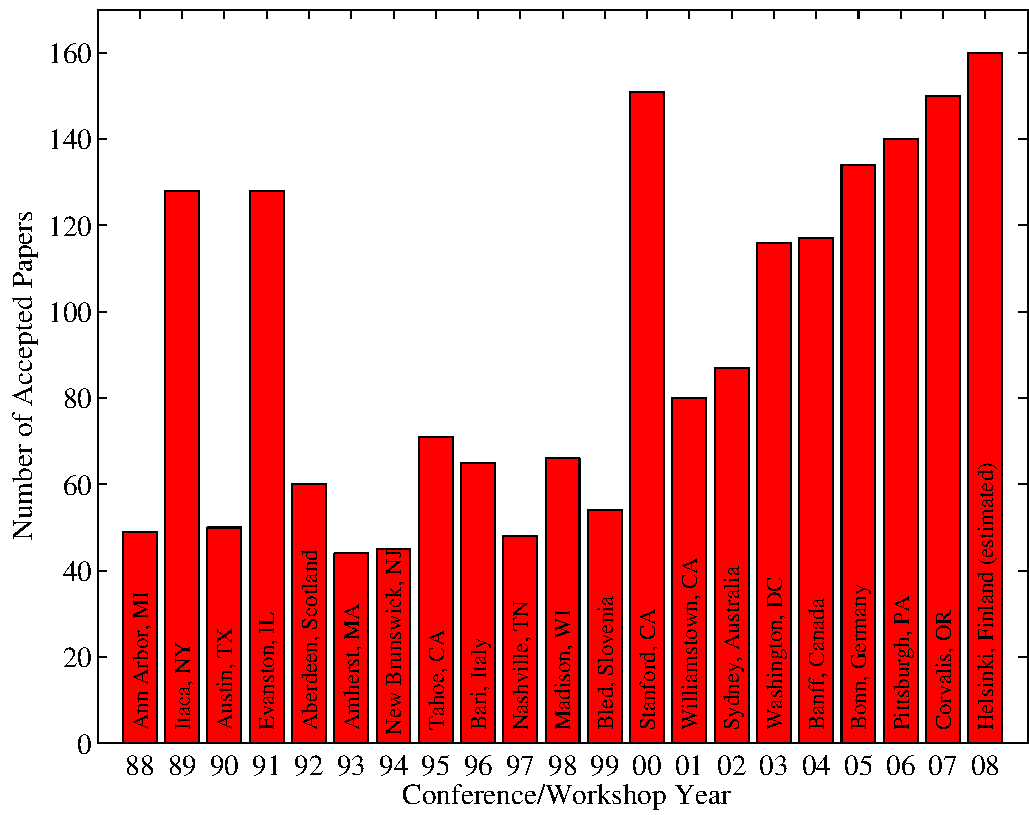
\includegraphics[width=\columnwidth]{icml_numpapers}}
% \caption{Historical locations and number of accepted papers for International
% Machine Learning Conferences (ICML 1993 -- ICML 2008) and International
% Workshops on Machine Learning (ML 1988 -- ML 1992). At the time this figure was
% produced, the number of accepted papers for ICML 2008 was unknown and instead
% estimated.}
% \label{icml-historical}
% \end{center}
% \vskip -0.2in
% \end{figure}

% \subsection{Figures}

% You may want to include figures in the paper to illustrate
% your approach and results. Such artwork should be centered,
% legible, and separated from the text. Lines should be dark and at
% least 0.5~points thick for purposes of reproduction, and text should
% not appear on a gray background.

% Label all distinct components of each figure. If the figure takes the
% form of a graph, then give a name for each axis and include a legend
% that briefly describes each curve. Do not include a title inside the
% figure; instead, the caption should serve this function.

% Number figures sequentially, placing the figure number and caption
% \emph{after} the graphics, with at least 0.1~inches of space before
% the caption and 0.1~inches after it, as in
% \cref{icml-historical}. The figure caption should be set in
% 9~point type and centered unless it runs two or more lines, in which
% case it should be flush left. You may float figures to the top or
% bottom of a column, and you may set wide figures across both columns
% (use the environment \texttt{figure*} in \LaTeX). Always place
% two-column figures at the top or bottom of the page.

% \subsection{Algorithms}

% If you are using \LaTeX, please use the ``algorithm'' and ``algorithmic''
% environments to format pseudocode. These require
% the corresponding stylefiles, algorithm.sty and
% algorithmic.sty, which are supplied with this package.
% \cref{alg:example} shows an example.

% \begin{algorithm}[tb]
%    \caption{Bubble Sort}
%    \label{alg:example}
% \begin{algorithmic}
%    \STATE {\bfseries Input:} data $x_i$, size $m$
%    \REPEAT
%    \STATE Initialize $noChange = true$.
%    \FOR{$i=1$ {\bfseries to} $m-1$}
%    \IF{$x_i > x_{i+1}$}
%    \STATE Swap $x_i$ and $x_{i+1}$
%    \STATE $noChange = false$
%    \ENDIF
%    \ENDFOR
%    \UNTIL{$noChange$ is $true$}
% \end{algorithmic}
% \end{algorithm}

% \subsection{Tables}

% You may also want to include tables that summarize material. Like
% figures, these should be centered, legible, and numbered consecutively.
% However, place the title \emph{above} the table with at least
% 0.1~inches of space before the title and the same after it, as in
% \cref{sample-table}. The table title should be set in 9~point
% type and centered unless it runs two or more lines, in which case it
% should be flush left.

% % Note use of \abovespace and \belowspace to get reasonable spacing
% % above and below tabular lines.

% \begin{table}[t]
% \caption{Classification accuracies for naive Bayes and flexible
% Bayes on various data sets.}
% \label{sample-table}
% \vskip 0.15in
% \begin{center}
% \begin{small}
% \begin{sc}
% \begin{tabular}{lcccr}
% \toprule
% Data set & Naive & Flexible & Better? \\
% \midrule
% Breast    & 95.9$\pm$ 0.2& 96.7$\pm$ 0.2& $\surd$ \\
% Cleveland & 83.3$\pm$ 0.6& 80.0$\pm$ 0.6& $\times$\\
% Glass2    & 61.9$\pm$ 1.4& 83.8$\pm$ 0.7& $\surd$ \\
% Credit    & 74.8$\pm$ 0.5& 78.3$\pm$ 0.6&         \\
% Horse     & 73.3$\pm$ 0.9& 69.7$\pm$ 1.0& $\times$\\
% Meta      & 67.1$\pm$ 0.6& 76.5$\pm$ 0.5& $\surd$ \\
% Pima      & 75.1$\pm$ 0.6& 73.9$\pm$ 0.5&         \\
% Vehicle   & 44.9$\pm$ 0.6& 61.5$\pm$ 0.4& $\surd$ \\
% \bottomrule
% \end{tabular}
% \end{sc}
% \end{small}
% \end{center}
% \vskip -0.1in
% \end{table}

% Tables contain textual material, whereas figures contain graphical material.
% Specify the contents of each row and column in the table's topmost
% row. Again, you may float tables to a column's top or bottom, and set
% wide tables across both columns. Place two-column tables at the
% top or bottom of the page.

% \subsection{Theorems and such}
% The preferred way is to number definitions, propositions, lemmas, etc. consecutively, within sections, as shown below.
% \begin{definition}
% \label{def:inj}
% A function $f:X \to Y$ is injective if for any $x,y\in X$ different, $f(x)\ne f(y)$.
% \end{definition}
% Using \cref{def:inj} we immediate get the following result:
% \begin{proposition}
% If $f$ is injective mapping a set $X$ to another set $Y$, 
% the cardinality of $Y$ is at least as large as that of $X$
% \end{proposition}
% \begin{proof} 
% Left as an exercise to the reader. 
% \end{proof}
% \cref{lem:usefullemma} stated next will prove to be useful.
% \begin{lemma}
% \label{lem:usefullemma}
% For any $f:X \to Y$ and $g:Y\to Z$ injective functions, $f \circ g$ is injective.
% \end{lemma}
% \begin{theorem}
% \label{thm:bigtheorem}
% If $f:X\to Y$ is bijective, the cardinality of $X$ and $Y$ are the same.
% \end{theorem}
% An easy corollary of \cref{thm:bigtheorem} is the following:
% \begin{corollary}
% If $f:X\to Y$ is bijective, 
% the cardinality of $X$ is at least as large as that of $Y$.
% \end{corollary}
% \begin{assumption}
% The set $X$ is finite.
% \label{ass:xfinite}
% \end{assumption}
% \begin{remark}
% According to some, it is only the finite case (cf. \cref{ass:xfinite}) that is interesting.
% \end{remark}
% %restatable

% \subsection{Citations and References}

% Please use APA reference format regardless of your formatter
% or word processor. If you rely on the \LaTeX\/ bibliographic
% facility, use \texttt{natbib.sty} and \texttt{icml2024.bst}
% included in the style-file package to obtain this format.

% Citations within the text should include the authors' last names and
% year. If the authors' names are included in the sentence, place only
% the year in parentheses, for example when referencing Arthur Samuel's
% pioneering work \yrcite{Samuel59}. Otherwise place the entire
% reference in parentheses with the authors and year separated by a
% comma \cite{Samuel59}. List multiple references separated by
% semicolons \cite{kearns89,Samuel59,mitchell80}. Use the `et~al.'
% construct only for citations with three or more authors or after
% listing all authors to a publication in an earlier reference \cite{MachineLearningI}.

% Authors should cite their own work in the third person
% in the initial version of their paper submitted for blind review.
% Please refer to \cref{author info} for detailed instructions on how to
% cite your own papers.

% Use an unnumbered first-level section heading for the references, and use a
% hanging indent style, with the first line of the reference flush against the
% left margin and subsequent lines indented by 10 points. The references at the
% end of this document give examples for journal articles \cite{Samuel59},
% conference publications \cite{langley00}, book chapters \cite{Newell81}, books
% \cite{DudaHart2nd}, edited volumes \cite{MachineLearningI}, technical reports
% \cite{mitchell80}, and dissertations \cite{kearns89}.

% Alphabetize references by the surnames of the first authors, with
% single author entries preceding multiple author entries. Order
% references for the same authors by year of publication, with the
% earliest first. Make sure that each reference includes all relevant
% information (e.g., page numbers).

% Please put some effort into making references complete, presentable, and
% consistent, e.g. use the actual current name of authors.
% If using bibtex, please protect capital letters of names and
% abbreviations in titles, for example, use \{B\}ayesian or \{L\}ipschitz
% in your .bib file.

% \section*{Accessibility}
% Authors are kindly asked to make their submissions as accessible as possible for everyone including people with disabilities and sensory or neurological differences.
% Tips of how to achieve this and what to pay attention to will be provided on the conference website \url{http://icml.cc/}.

% \section*{Software and Data}

% If a paper is accepted, we strongly encourage the publication of software and data with the
% camera-ready version of the paper whenever appropriate. This can be
% done by including a URL in the camera-ready copy. However, \textbf{do not}
% include URLs that reveal your institution or identity in your
% submission for review. Instead, provide an anonymous URL or upload
% the material as ``Supplementary Material'' into the OpenReview reviewing
% system. Note that reviewers are not required to look at this material
% when writing their review.

% % Acknowledgements should only appear in the accepted version.
% \section*{Acknowledgements}

% \textbf{Do not} include acknowledgements in the initial version of
% the paper submitted for blind review.

% If a paper is accepted, the final camera-ready version can (and
% probably should) include acknowledgements. In this case, please
% place such acknowledgements in an unnumbered section at the
% end of the paper. Typically, this will include thanks to reviewers
% who gave useful comments, to colleagues who contributed to the ideas,
% and to funding agencies and corporate sponsors that provided financial
% support.


% % In the unusual situation where you want a paper to appear in the
% % references without citing it in the main text, use \nocite
% \nocite{langley00}
\newlength{\imgsize}
\begin{abstract}
There is a widely-spread claim that GANs are difficult to train, and GAN architectures in the literature are littered with empirical tricks. We provide evidence against this claim and build a modern GAN baseline in a more principled manner. First, we derive a well-behaved regularized relativistic GAN loss that addresses issues of mode dropping and non-convergence that were previously tackled via a bag of ad-hoc tricks. We analyze our loss mathematically and prove that it admits local convergence guarantees, unlike most existing relativistic losses. Second, this loss allows us to discard all ad-hoc tricks and replace outdated backbones used in common GANs with modern architectures. Using StyleGAN2 as an example, we present a roadmap of simplification and modernization that results in a new minimalist baseline---\modelName (``Re-GAN''). Despite being simple, our approach surpasses StyleGAN2 on FFHQ, ImageNet, CIFAR, and Stacked MNIST datasets, and compares favorably against state-of-the-art GANs and diffusion models.\\
Code: \href{https://www.github.com/brownvc/R3GAN}{https://www.github.com/brownvc/R3GAN}
\end{abstract}
\vspace{-3ex}
%
\section{Introduction}
%
% Problem
Time series modeling is a well-established problem, with tasks such as forecasting and classification motivated by many domains such as healthcare, finance, and engineering~\citep{shumway2000time}. 
% Furthermore, time series data is diverse and readily available, presenting an exciting modality to learn from.
% Why interesting, important, and hard
However, effective time series modeling presents several challenges: 
% Methods often must be expressive, able to forecast arbitrary horizons, and efficient.
% itemsep=0.1pt,
\begin{itemize}[leftmargin=*]
% \begin{itemize}[itemsep=0.1pt, topsep=0pt,leftmargin=*]
\item First, 
% to effectively model time series data, 
methods should \textbf{expressively} capture complex, long-range, and \emph{autoregressive} dependencies. 
Time series data often reflects higher order dependencies, seasonality, and trends, governing how past samples determine future terms~\citep{chatfield2000time}. 
This motivates many classical approaches 
% and deep learning methods~\citep{zhou2022film, zhou2022fedformer, woo2022etsformer} 
that model these properties~\citep{box1970time, winters1960forecasting}, alongside expressive deep learning mechanisms such as attention~\citep{vaswani2017attention} and fully connected layers that model interactions between \emph{every} sample in an input sequence~\citep{zeng2022transformers}.
%
\item Second, 
% for forecasting, 
methods
% to tackle a wide range of time series data domains and tasks, 
% methods
should be able to forecast a wide range of \textbf{long horizons} over various data domains. 
% \eg{} to handle various forecasting horizons,
% and data domains,  
% methods should be (ii) \emph{broadly and easily applicable}, 
% without costly manual oversight or overly-specialized architectural changes. 
% without costly or overspecialized architectural changes. 
Reflecting real world demands, popular forecasting benchmarks evaluate methods on
% across 58 datasets with individual target horizons~\citep{godahewa2021monash} or 
\numberMonashTasks{} different tasks~\citep{godahewa2021monash} and 24$-$960 time-step horizons~\cite{zhou2021informer}. 
Furthermore, as testament to accurately learning time series processes, 
% as a test for learning time series,
forecasting methods should ideally
% should thus handle long horizons, and ideally 
% continuously 
also be able to predict future time-steps on horizons they were not explicitly trained on.
% ideally without the need for additional retraining and architectural adaptation. 
% with fixed input sequences. 
% Classification and forecasting methods should generalize to various datasets.
%
\item Finally, methods should be \textbf{efficient} with training and inference. Many time series applications require processing very long sequences, \eg{} classifying audio data with sampling rates up to $16{,}000$ Hz \citep{warden2018speech}. 
To handle such settings---where we still need large enough models that can expressively model this data---training and inference should ideally scale \emph{subquadratically} with sequence length and model size in time and space complexity.
% Efficient training over long sequences is a fundamental challenge for deep learning, where popular Transformers 
%To thus effectively learn from such time series on modern hardware, we require fast inference that fits memory constraints.
\end{itemize}

% Why prior stuff isn't sufficient
Unfortunately, existing time series methods struggle to achieve all three criteria.  
%
Classical methods (\cf{} ARIMA~\citep{box1970time}, exponential smoothing (ETS)~\citep{winters1960forecasting}) often require manual data preprocessing and model selection to identify expressive-enough models. 
%To effectively scale across all such evaluations, we ideally can avoid added complexities with a single simple architecture.
%
Deep learning methods commonly train to predict specific horizon lengths, \ie{} as \emph{direct multi-step forecasting}~\citep{https://doi.org/10.1111/j.1467-6419.2007.00518.x}, and we find this hurts their ability to forecast longer horizons (Sec. \ref{sec:empirical_horizons}).  
% On applicability, 
% state-of-the-art neural nets often introduce specialized architectures to handle specific data properties~\citep{liu2022pyraformer,zhou2022film}. 
%
They also face limitations achieving high expressivity \emph{and} efficiency. Fully connected networks (FCNs) such as NLinear \cite{zeng2022transformers} scale quadratically in $\mathcal{O}(\ell h)$ space complexity (with input length $\ell$ and forecast length $h$). 
%
Recent Transformer-based models reduce this complexity to $\mathcal{O}(\ell + h)$, but do not always outperform the aforementioned fully connected networks on forecasting benchmarks~\citep{liu2022pyraformer, zhou2021informer}. 
%

% , despite introducing various specific architectures to improve expressiveness or efficiency~\citep{ zhou2022film, zhou2022fedformer, woo2022etsformer}.
% However, they rarely obtain higher MSE over FCNs on benchmarks, and introduce various specific architectures and processing steps.


% Deep learning methods may be highly expressive but are either non-generic by adding specialized architectures to deal with different data properties (\eg{} trends, seasonality) and tasks (\eg{} classification, forecasting, forecasting with different horizons) or are not efficient at processing long sequences. For example, fully-connected networks in \cite{zeng2022transformers} are highly expressive and achieve state-of-the-art results on many forecasting benchmarks; however, their time and space complexity scales quadratically in input sequence length and forecast horizon length. Transformer variations bring down this complexity to near linear in compute and memory~\citep{liu2022pyraformer, zhou2021informer}; however, they rarely obtain higher MSE over FCNs on benchmarks, and introduce various specific architectures and processing steps~\citep{zhou2022film, zhou2022fedformer, woo2022etsformer}.

\begin{figure}[!t]
  \centering
%   \includegraphics[width=1\textwidth]{_ICLR2023_paper/figures/figure_pull_2layer_v1.2.pdf}
  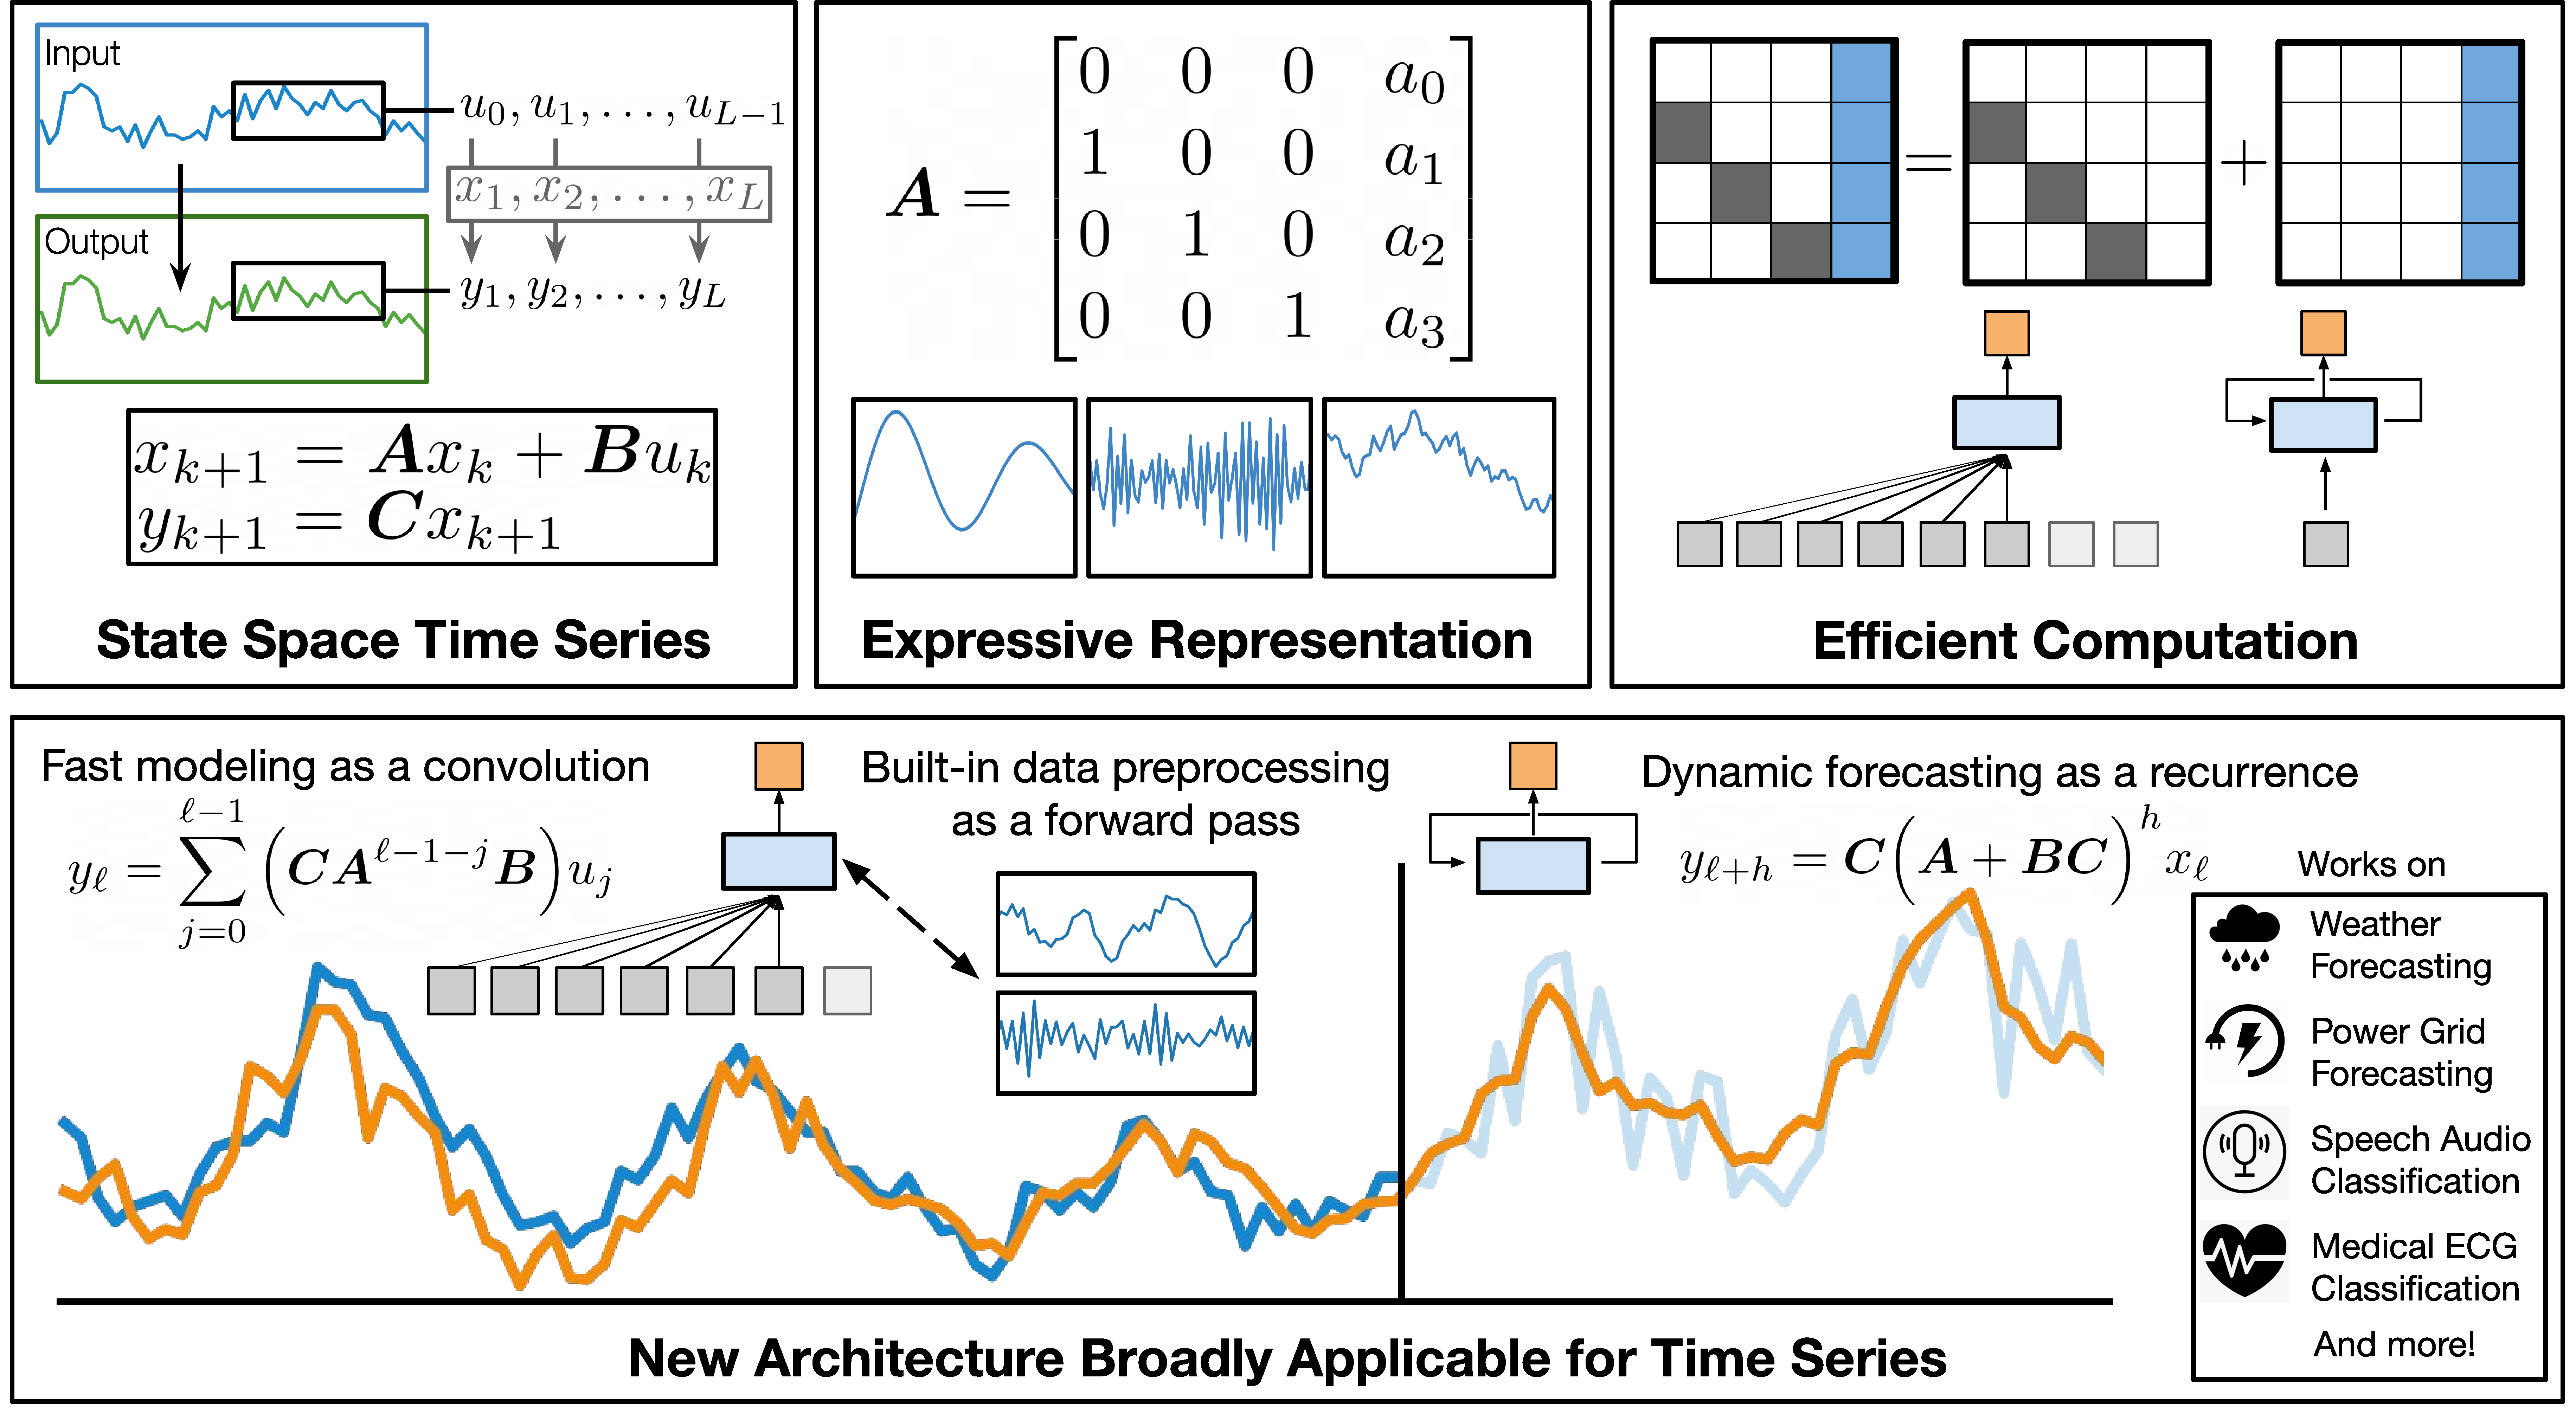
\includegraphics[width=1\textwidth]{_ICLR2023_paper/figures/time_series_ssm_use_this_2_levels_refactor1.pdf}
 \caption{We learn time series processes as state-space models (SSMs) (\textbf{top left}). We represent SSMs with the \textit{companion matrix}, which is a highly expressive representation for discrete time series  (\textbf{top middle}), and compute such SSMs efficiently as convolutions or recurrences via a shift + low-rank decomposition (\textbf{top right}). We use these SSMs to build \ourmethod{}, a new time series architecture broadly effective across tasks and domains (\textbf{bottom}).}
  \label{fig:overvew_fig1}
\end{figure}

% Our Method
%
% We thus propose \textbf{\ourmethod{}}, a new deep learning time series architecture. 
%
% Towards more effective time series modeling, 



We thus propose \textbf{\textsc{SpaceTime}}, a deep state-\textbf{space} architecture for effective \textbf{time} series modeling. 
% For more accurate forecasting and classification, 
To achieve this,
we focus on improving each criteria via three core contributions:

% \begin{enumerate}[itemsep=0.1pt,topsep=0pt,leftmargin=*]
\begin{enumerate}[topsep=0pt,leftmargin=*]
    \item For expressivity, our key idea and building block is a linear layer that models time series processes as \emph{state-space models} (SSMs) via the \emph{companion matrix} (Fig.~\ref{fig:overvew_fig1}). 
    We start with SSMs due to their connections to both classical time series analysis~\citep{kalman1960new, hamilton1994state} and recent deep learning advances~\citep{gu2021efficiently}. Classically, many time series models such as ARIMA and exponential smoothing (ETS) can be expressed as SSMs~\citep{box1970time, winters1960forecasting}. 
    Meanwhile, recent state-of-the-art deep sequence models~\citep{gu2021efficiently} have used SSMs to outperform Transformers and LSTMs on challenging long-range benchmarks~\citep{tay2020long}.
    % Meanwhile, recent SSM-based deep learning models~\citep{gu2021efficiently} have achieved state-of-the-art sequence modeling on challenging long-range benchmarks~\citep{tay2020long}. 
    Their primary innovations show how to formulate SSMs as neural network parameters that are practical to train. However, we find limitations with these deep SSMs for time series data. While we build on their advances, we prove that these prior SSM representations~\citep{ gu2021combining, gu2021efficiently, gupta2022diagonal}
    % cite these later: rangapuram2018, salinas2020deepar, lin2021ssdnet,
    cannot capture autoregressive processes fundamental for time series. We thus specifically propose the companion matrix representation for its expressive and memory-efficient properties. 
    We prove that the companion matrix SSM recovers fundamental autoregressive (AR) and smoothing processes modeled in classical techniques such as ARIMA and ETS, while only requiring $\mathcal{O}(d)$ memory to represent an $\mathcal{O}(d^2)$ matrix. 
    Thus, \ourmethod{} inherits the benefits of prior SSM-based sequence models, while introducing improved expressivity that 
    recovers fundamental time series processes
    % apture multiple AR processes and data preprocessing techniques 
    simply through its layer weights. 
    
    \item 
    % For forecasting over long horizons, we introduce a new ``closed-loop'' view of SSMs. Previous architectures apply the SSM in an ``open-loop'' fashion \citep{gu2021efficiently}, where the output is driven by the input sequence. 
    % However, to continuously forecast to long horizons, we require that the SSM has the ability to continue forecasting the signal in the absence of an input at those time steps. 
    % Inspired by classical closed-loop control~\citep{doyle2013feedback,aastrom2021feedback}, we propose a new variant of SSMs that explicitly models the next time-step input, which enables a multi-layer \ourmethod{} network to recurrently output long horizons.
    For forecasting long horizons, we introduce a new ``closed-loop'' view of SSMs. Prior deep SSM architectures either apply the SSM as an ``open-loop'' \citep{gu2021efficiently}, where fixed-length inputs necessarily generate same-length outputs, or use closed-loop autoregression where final layer outputs are fed through the \emph{entire} network as next-time-step inputs~\citep{goel2022s}. 
    We describe issues with both approaches in Sec.~\ref{sec:forecasting_ssm}, and instead achieve autogressive forecasting in a deep network with only a single SSM layer. We do so by explicitly training the SSM layer to predict its next time-step \emph{inputs}, alongside its usual outputs. This allows the SSM to recurrently generate its own future inputs that lead to desired outputs---\ie{} those that match an observed time series---so we can forecast over many future time-steps without explicit data inputs. 
    % This allows \ourmethod{} to generate its own final-layer inputs for outputting forecasts over many future time-steps.

    \item For efficiency, we introduce an algorithm for efficient training and inference with the companion matrix SSM. We 
    % first show how the companion SSM can be computed as both a convolution and a recurrence for layer-wise forward passes and forecasting respectively.  
    exploit the companion matrix's structure as a ``shift plus low-rank'' matrix, which allows us to reduce the time and space complexity for computing SSM hidden states and outputs from $\tilde{\mathcal{O}}(d \ell )$ to $\tilde{\mathcal{O}}(d + \ell)$ in SSM state size $d$ and input sequence length $\ell$. 
\end{enumerate}
% To subsequently build a full \ourmethod{} model, we simply stack together multiple layers---which each parametrize multiple companion matrix SSMs---into  a standard encoder-decoder architecture. 

% Simply stacking these layers together into a standard encoder-decoder architecture thus builds a highly expressive and efficient time series model.

In experiments, 
% we evaluate \ourmethod{} on extensive time series forecasting and classification tasks, and test if \ourmethod{}'s contributions empirically lead to (1) expressive time series modeling, (2) long-horizon forecasting, and (3) efficient training. 
%
we find \ourmethod{} consistently obtains state-of-the-art or near-state-of-the-art results, achieving best or second-best AUROC on 6 out of 7 ECG and audio speech time series classification tasks, and best mean-squared error (MSE) on 14 out of 16 Informer benchmark forecasting tasks~\citep{zhou2021informer}. \ourmethod{} also sets a new best average ranking across \numberMonashTasks{} tasks on the Monash benchmark~\citep{godahewa2021monash}.  
% 
We connect these gains with improvements on our three effective time series modeling criteria.  %
For expressivity, on synthetic ARIMA processes \ourmethod{} learns AR processes that prior deep SSMs cannot. 
%
% via extensive synthetics. As a controlled benchmark for expressiveness, we test how well popular architectures can fit standard AR processes, and find that \ourmethod{} best learns the true time series processes via its companion matrix SSM.
% compared to prior deep SSM representations.
%via visualizations of the process's ground-truth transfer function versus those parameterized by the trained SSM weights.
%
%
For long horizon forecasting, \ourmethod{} consistently outperforms prior state-of-the-art on the longest horizons by large margins. \ourmethod{} also generalizes better to \emph{new} horizons not used for training.
%
% validate that 
% We then validate (2) by showing that trained \ourmethod{}s generalize better to new horizons that models were not trained for. We also find that on the Informer benchmark, \ourmethod{} consistently outperforms alternatives on the longest evaluation horizons by the largest margins, up to $\textbf{X}$\% relative reduction in MSE for forecasting $\textbf{Y}$ time-steps.
%
% best RMSE on 25 out of 30 tasks from the diverse Monash benchmark~\citep{godahewa2021monash}.
% setting a new record among prior classical and deep learning approaches. 
% Moreover, we find that \ourmethod{} improves forecasts to arbitrary horizons (that it was not trained on) by \%XX on the Informer benchmark. 
For efficiency, on speed benchmarks \ourmethod{} obtains 73\% and 80\% relative wall-clock speedups over parameter-matched Transformers and LSTMs respectively, when training on real-world ETTh1 data.



%------------------------------------------------------------------------
\section{Serving Two Masters: Stability and Diversity with RpGAN \texorpdfstring{$+ R_1+R_2$}{R-1R-2}}
%---An Improved Training Objective \vk{title can be tweaked; i recommend naming your new loss}}
% James Tompkin: I wrote 'serving two masters'. Note that 'serving two masters' is inherently a religious label; in the bible, Matthew writes that one cannot serve two masters (only God). In the traditions of monarchy (to which our title alludes in the procession of kings), a king had divine right and so avoided this problem of serving two masters (to serve God and to serve one's king is to serve two masters, except once we establish that kings are divine then this problem goes away as the same master - God - is then being served). I am not religious.
\label{sec:loss}

In defining a GAN objective, we tackle two challenges: stability and diversity. Some previous work deals with stability~\cite{sg1,sg2,sg3} and other previous work deals with mode collapse \cite{rgan}. We combine a stable method with a simple regularizer grounded by theory to overcome both.

\vspace{-1ex}
\subsection{Traditional GAN}
\vspace{-1ex}
A traditional GAN~\cite{gan,nowozin2016f} is formulated as a minimax game between a discriminator $D_\psi$ and a generator $G_\theta$. Given real data $x\sim p_\mathcal{D}$ and fake data $x\sim p_\theta$ produced by $G_\theta$, the most general form of a GAN is given by:
\begin{align}
\begin{split}
\label{eq:gan}
\resizebox{0.438\textwidth}{!}{$
\mathcal{L}(\theta,\psi)=\mathbb{E}_{z\sim p_z}\left[f\left(  D_\psi(G_\theta(z))\right)\right]+\mathbb{E}_{x\sim p_\mathcal{D}}\left[f\left( -D_\psi(x) \right)\right]
$}
\end{split}
\end{align}
\noindent where $G$ tries to minimize $\mathcal{L}$ while $D$ tries to maximize it. The choice of $f$ is flexible~\cite{lsgan,hingegan}. In particular, $f(t) = -\log(1+e^{-t})$ recovers the classic GAN by Goodfellow~\etal~\cite{gan}. For the rest of this work, this will be our choice of $f$~\cite{nowozin2016f}.

% It is shown that Eq.\ref{eq:gan} is actually convex if we can directly optimize $p_\theta$~\cite{gan,rpgan}. Though in practice, the empirical GAN loss moves fake samples past the decision boundary induced by $D$ rather than updating the density function $p_\theta$ directly. This turns out to be a much harder problem that is susceptible to two common failure cases: mode collapse/dropping\footnote{Mode collapse and mode dropping are technically two related yet distinct problems. We use these two terms interchangeably hereafter to refer to the general problem where $\supp p_\theta$ fails to fully cover $\supp p_\mathcal{D}$.} and non-convergence. \vk{Minor thing: could provide a bit more information (1 sentence) on mode dropping and collapse}
It has been shown that Equation~\ref{eq:gan} has convex properties when $p_\theta$ can be optimized directly~\cite{gan,rpgan}. However, in practical implementations, the empirical GAN loss typically shifts fake samples beyond the decision boundary set by $D$, as opposed to directly updating the density function $p_\theta$. This deviation leads to a significantly more challenging problem, characterized by susceptibility to two prevalent failure scenarios: mode collapse/dropping\footnote{While mode collapse and mode dropping are technically distinct issues, they are used interchangeably in this context to describe the common problem where $\supp\ p_\theta$ does not fully cover $\supp\ p_\mathcal{D}$.} and non-convergence.

\vspace{-1ex}
\subsection{Relativistic \texorpdfstring{$f$-GAN}{f-GAN}.}
\vspace{-1ex}
% We adopt relativistic pairing GAN (RpGAN) by Jolicoeur-Martineau~\etal~\cite{rgan} as the main GAN loss. 
% Sun~\etal showed that RpGAN is especially effective against mode dropping~\cite{rpgan} as the loss landscape of RpGAN contains no local minima that correspond to mode dropping solutions. 
% Next, we apply zero-centered gradient penalties~\cite{r1,r1r2} to RpGAN. Gradient penalty is a well known technique that stabilizes GAN training~\cite{wgan-gp,r1r2,r1} and has been proven to be crucial to GAN convergence~\cite{r1}. As our contribution to the theory, we follow Mescheder~\etal~\cite{r1} and prove that gradient-penalized RpGAN enjoys the same guarantee of local convergence as regularized classic GANs. In addition to theoretical guarantees, our empirical results suggest that gradient penalized RpGAN is sufficiently well-behaved, to the extent that allows us to remove all GAN tricks without encountering non-convergence or mode dropping.

We employ a slightly different minimax game named relativistic pairing GAN (RpGAN) by Jolicoeur-Martineau~\etal~\cite{rgan} to address mode dropping. The general RpGAN is defined as:
\begin{equation}
\label{eq:rpgan}
\mathcal{L}(\theta,\psi)=\mathbb{E}_{\substack{z\sim p_z\\x\sim p_\mathcal{D}}}\left[f\left(  D_\psi(G_\theta(z))-D_\psi(x) \right)\right]
\end{equation}
Although Eq.\ref{eq:rpgan} differs only slightly from Eq.\ref{eq:gan}, evaluating the critic difference has a fundamental impact on the landscape of $\mathcal{L}$. Since Eq.\ref{eq:gan} merely requires $D$ to separate real and fake data, in the scenario where all real and fake data can be separated by a single decision boundary, the empirical GAN loss encourages $G$ to simply move all fake samples barely past this single boundary---this degenerate solution is what we observe as mode collapse/dropping. Sun~\etal~\cite{rpgan} characterize such degenerate solutions as bad local minima in the landscape of $\mathcal{L}$, and show that Eq.\ref{eq:gan} has \emph{exponentially many} bad local minima. The culprit is the existence of a single decision boundary that naturally arises when real and fake data are considered in isolation. RpGAN introduces a simple solution by coupling real and fake data,~\ie a fake sample is critiqued by its realness \emph{relative to} a real sample, which effectively maintains a decision boundary in the neighborhood of \emph{each} real sample and hence forbids mode dropping. Sun~\etal~\cite{rpgan} show that the landscape of Eq.\ref{eq:rpgan} contains no local minima that correspond to mode dropping solutions, and that every basin is a global minimum.

\vspace{-1ex}
\subsection{Training Dynamics of RpGAN}
\vspace{-1ex}
Although the landscape result~\cite{rpgan} of RpGAN allows us to address mode dropping, the training dynamics of RpGAN have yet to be studied. The ultimate goal of Eq.~\ref{eq:rpgan} is to find the equilibrium $(\theta^*,\psi^*)$ such that $p_{\theta^*}=p_\mathcal{D}$ and $D_{\psi^*}$ is constant everywhere on $p_\mathcal{D}$. Sun~\etal~\cite{rpgan} show that $\theta^*$ is globally reachable along a non-increasing trajectory in the landscape of Eq.\ref{eq:rpgan} under reasonable assumptions. However, the existence of such a trajectory does not necessarily mean that gradient descent will find it. Jolicoeur-Martineau~\etal show empirically that unregularized RpGAN does not perform well~\cite{rgan}. 

\vspace{0.5ex}
\noindent \textbf{Proposition~\upperRomannumeral{1}.} (Informal) \emph{Unregularized RpGAN does not always converge using gradient descent.}
%\vk{Propositions should ideally be made precise or in the worst case, say it's an informal statement (but then you still have to make it intuitively understandable)}
\vspace{0.5ex}

\noindent We confirm this proposition with a proof in Appendix H. 
% In summary, we follow Mescheder~\etal~\cite{r1} and inherit their DiracGAN counterexample to apply it to RpGAN. 
We show analytically that RpGAN does not converge for certain types of $p_\mathcal{D}$, such as ones that approach a delta distribution. Thus, further regularization is necessary to fill in the missing piece of a well-behaved loss.

\vspace{-1.5ex}
\paragraph{Zero-centered gradient penalties.}
To tackle RpGAN non-convergence, we explore gradient penalties as the solution since it is proven that zero-centered gradient penalties (0-GP) facilitate convergent training for classic GANs~\cite{r1}. The two most commonly-used 0-GPs are $R_1$ and $R_2$:
\begin{equation}
\begin{aligned}
R_1(\psi)&=\frac{\gamma}{2}\mathbb{E}_{x\sim p_\mathcal{D}}\left[\left\| \nabla_x D_\psi \right \|^2\right]\\ 
R_2(\theta,\psi)&=\frac{\gamma}{2}\mathbb{E}_{x\sim p_\theta}\left[\left\| \nabla_x D_\psi \right \|^2\right]
\end{aligned}
\end{equation}
$R_1$ penalizes the gradient norm of $D$ on real data, and $R_2$ on fake data. Analysis on the training dynamics of GANs has thus far focused on local convergence~\cite{nagarajan2017gradient,gannum,r1},~\ie whether the training at least converges when $(\theta,\psi)$ are in a neighborhood of $(\theta^*,\psi^*)$. In such a scenario, the convergence behavior can be analyzed~\cite{nagarajan2017gradient,gannum,r1} by examining the spectrum of the Jacobian of the gradient vector field $\left(-\nabla_\theta\mathcal{L},\nabla_\psi\mathcal{L} \right )$ at $(\theta^*,\psi^*)$. The key insight here is that when $G$ already produces the true distribution, we want $\nabla_x D=0$, so that $G$ is not pushed away from its optimal state, and thus the training does not oscillate. $R_1$ and $R_2$ impose such a constraint when $p_\theta=p_\mathcal{D}$. This also explains why earlier attempts at gradient penalties, such as the one-centered gradient penalty (1-GP) in WGAN-GP~\cite{wgan-gp}, fail to achieve convergent training~\cite{r1} as they still encourage $D$ to have a non-zero slope when $G$ has reached optimality.

Since the same insight also applies to RpGAN, 
we extend our previous analysis and show that:
% our goal is to extend the proof of Mescheder~\etal~\cite{r1} to RpGAN and show that:

\vspace{0.5ex}
\noindent \textbf{Proposition~\upperRomannumeral{2}.} (Informal) \emph{RpGAN with $R_1$ or $R_2$ regularization is locally convergent subject to similar assumptions as in} Mescheder~\etal~\cite{r1}.
\vspace{0.5ex}

In Appendix I, our proof similarly analyzes the eigenvalues of the Jacobian of the regularized RpGAN gradient vector field at $(\theta^*,\psi^*)$. We show that all eigenvalues have a negative real part; thus, regularized RpGAN is convergent in a neighborhood of $(\theta^*,\psi^*)$ for small enough learning rates~\cite{r1}.

\vspace{-1ex}
\paragraph{Discussion.}
Another line of work~\cite{r1r2} links $R_1$ and $R_2$ to instance noise~\cite{instancenoise} as its analytical approximation. Roth et al.~\cite{r1r2} showed that for the classic GAN~\cite{gan} by Goodfellow~\etal, $R_1$ approximates convolving $p_\mathcal{D}$ with the density function of $\mathcal{N}(0, \gamma I)$, up to additional weighting and a Laplacian error term. $R_2$ likewise approximates convolving $p_\theta$ with $\mathcal{N}(0, \gamma I)$ up to similar error terms. The Laplacian error terms from $R_1$, $R_2$ cancel when $D_\psi$ approaches $D_{\psi^*}$. We do not extend Roth~\etal's proof~\cite{r1r2} to RpGAN; however, this approach might provide complimentary insights to our work, which follows the strategy of Mescheder~\etal~\cite{r1}. 

We demonstrate our loss in Appendix A where we focus on practical considerations such as global convergence. Building on Roth et al.~\cite{r1r2}, we apply both $R_1$ and $R_2$ to improve global stability.
% \begin{figure}
%     \centering
%     \includegraphics{figures/FID-vs-Params-Plot.eps}
%     \caption{This scatter-plot shows the FID performance of our model on FFHQ-256 vs the number of parameters when only trained for 5million steps}
%     \label{fig:fid-vs-params-ablation}
% \end{figure}


\section{A Roadmap to a New Baseline --- \modelName}
\label{sec:roadmap}

% \vk{What about naming the new GAN that is being proposed? SimpleGAN...?}\jt{R3GAN...?}

% \vk{My main comment about this section is that it reads like mix of methods and experiments: all the experimental details/results (e.g., we set the learning rate to $10^{-4}$) should be under experiments (but you can still describe the key important takeaways here, e.g., we need a smaller learning rate)}

The well-behaved RpGAN + $R_1$ + $R_2$ loss alleviates GAN optimization problems, and lets us proceed to build a minimalist baseline---\modelName---with recent network backbone advances in mind~\cite{convnext,metaformer}. Rather than simply state the new approach, we will draw out a roadmap from the StyleGAN2 baseline~\cite{sg2ada}. This model (Config A; identical to~\cite{sg2ada}) consists of a VGG-like~\cite{vgg} backbone for $G$, a ResNet $D$, a few techniques that facilitate style-based generation, and many tricks that serve as patches to the weak backbone. Then, we remove all non-essential features of StyleGAN2 (Config B), apply our loss function (Config C), and gradually modernize the network backbone (Config D-E).


We evaluate each configuration on FFHQ $256\times256$~\cite{sg1}. Network capacity is kept roughly the same for all configurations---both $G$ and $D$ have about 25M trainable parameters. Each configuration is trained until $D$ sees 5M real images. We inherit training hyperparameters (optimizer settings, batch size, EMA decay length,~\etc) from Config A unless otherwise specified. We tune the training hyperparameters for our final model and show the converged result in Sec.~\ref{sec:exp}.

%\paragraph{StyleGAN2 (Config A).}This configuration is identical to the baseline~\cite{sg2ada} with the style-based generator and all tricks enabled.  

\vspace{-1ex}
\paragraph{Minimum Baseline (Config B).}
We strip away all StyleGAN2 features, retaining only the raw network backbone and basic image generation capability. The features fall into three categories:
\begin{itemize}[leftmargin=10pt,itemsep=0pt,topsep=0pt]
\item Style-based generation: mapping network~\cite{sg1}, style injection~\cite{sg1}, weight modulation/demodulation~\cite{sg2}, noise injection~\cite{sg1}.
\end{itemize}\quad % JT: Weird but intential LaTeX
\begin{itemize}[leftmargin=10pt,itemsep=0pt,topsep=0pt]
\vspace{-0.25cm} % JT: Weird but intential LaTeX
\item Image manipulation enhancements: mixing regularization~\cite{sg1}, path length regularization~\cite{sg2}.
\item Tricks: $z$ normalization~\cite{pggan}, minibatch stddev~\cite{pggan}, equalized learning rate~\cite{pggan}, lazy regularization~\cite{sg2}.
\end{itemize}

% Such features could be reintroduced as per application need (e.g., style injection). 
Following~\cite{sgxl,sg-t}, we reduce the dimension of $z$ to 64. The absence of equalized learning rate necessitates a lower learning rate, reduced from $2.5\times10^{-3}$ to $5\times10^{-5}$. Despite a higher FID of 12.46 than Config-A, this simplified baseline produces reasonable sample quality and stable training. We compare this with DCGAN~\cite{dcgan}, an early attempt at image generation. Key differences include:
\begin{enumerate}[label=\alph*), noitemsep,topsep=0pt,leftmargin=24pt]
\item Convergent training objective with $R_1$ regularization.\label{item:convergent} 
\item Smaller learning rate, avoiding momentum optimizer (Adam $\beta_1=0$).\label{item:learning_rate} 
\item No normalization layer in $G$ or $D$.\label{item:normalization} 
\item Proper resampling via bilinear interpolation instead of strided (transposed) convolution.\label{item:resampling} 
\item Leaky ReLU in both $G$ and $D$, no tanh in the output layer of $G$.\label{item:activation} 
\item $4\times4$ constant input for $G$, output skips for $G$, ResNet $D$.\label{item:input} 
\end{enumerate}

We discuss our findings about these principles in Appendix B and establish that \ref{item:convergent} through \ref{item:activation} are critical to the success of StyleGAN2, and apply them to all subsequent configurations.

\paragraph{Well-behaved loss function (Config C).}
% Given the simplified baseline, we move on to the modernization part of the roadmap. We first modernize the loss function so that the representation power of modern network backbones will not be compromised by GAN optimization difficulties. 
We use the loss function proposed in Section~\ref{sec:loss} and this reduces FID to 11.65. We hypothesize that the network backbone in Config B is the limiting factor. 
% and expect more drastic improvements as further modernization takes place.

\paragraph{General network modernization (Config D).}
First, we apply the 1-3-1 bottleneck ResNet architecture~\cite{resnet,resnet2} to both $G$ and $D$. This is the direct ancestor of all modern vision backbones~\cite{convnext,metaformer}. 
% However, rather than precisely replicating the architecture in~\cite{resnet2}, 
We also incorporate principles discovered in Config B and various modernization efforts from ConvNeXt~\cite{convnext}. We categorize the roadmap of ConvNeXt as follows:
% \begin{enumerate}[label=\roman*)]
%     \item Consistently beneficial: 1) increased width with depthwise conv. 2) inverted bottleneck. 3) fewer activation functions. 4) separate resampling layers.
%     \item Negligible performance gain: 1) large kernel depthwise conv with fewer channels. 2) replacing ReLU with GELU. 3) fewer normalization layers. 4) replacing batch norm with layer norm.
%     \item Irrelevant to our problem setting: 1) improved training recipe. 2) stage ratio. 3) "patchify" stem.
% \end{enumerate}
% % We are interested in applying i) to our model, among which i.3) and i.4) are applicable to the classic ResNet. We leave i.1) and i.2) for Config E. Much of ii) were introduced merely for the sake of mimicking vision transformers~\cite{swin,vit} even though they fail to bring any significant improvement~\cite{convnext}. ii.3) and ii.4) are inapplicable since we do not use any normalization layer following principle c). ii.2) is directly at odds with our finding that GELU deteriorates GAN performance, and we use leaky ReLU as in principle e). Liu~\etal put heavy emphasis on using large conv kernels (ii.1)~\cite{convnext}, however this results in slightly but consistently worse performance than using wider $3\times3$ conv layers and we therefore do not employ this design choice of ConvNeXt.

% We aim to apply i) to our model, specifically i.3) and i.4) for the classic ResNet, while reserving i.1) and i.2) for Config E. Many aspects of ii) were introduced merely to mimic vision transformers~\cite{swin,vit} without yielding significant improvements~\cite{convnext}. ii.3) and ii.4) are inapplicable due to our avoidance of normalization layers following principle c). ii.2) contradicts our finding that GELU deteriorates GAN performance, thus we use leaky ReLU per principle e). Liu~\etal emphasize large conv kernels (ii.1)~\cite{convnext}, but this results in slightly worse performance compared to wider $3\times3$ conv layers, so we do not adopt this ConvNeXt design choice.
%
\begin{enumerate}[label=\roman*., itemsep=2pt,leftmargin=12pt,topsep=0pt]
    \item Consistently beneficial: \begin{enumerate*}[label=\theenumi\arabic*), ref=\arabic*, before=\unskip{ }, itemjoin={{, }}, itemjoin*={{, and }}]
        \item\label{item:i1} increased width with depthwise conv.
        \item\label{item:i2} inverted bottleneck
        \item\label{item:i3} fewer activation functions
        \item\label{item:i4} separate resampling layers
    \end{enumerate*}
    \item Negligible performance gain: \begin{enumerate*}[label=\theenumi\arabic*), ref=\arabic*, before=\unskip{ }, itemjoin={{, }}, itemjoin*={{, and }}]
        \item\label{item:ii1} large kernel depthwise conv.~with fewer channels
        \item\label{item:ii2} swap ReLU with GELU
        \item\label{item:ii3} fewer normalization layers
        \item\label{item:ii4} swap batch norm.~with layer norm.
    \end{enumerate*}
    \item Irrelevant to our setting: \begin{enumerate*}[label=\theenumi\arabic*), ref=\arabic*, before=\unskip{ }, itemjoin={{, }}, itemjoin*={{, and }}]
        \item\label{item:iii1} improved training recipe
        \item\label{item:iii2} stage ratio
        \item\label{item:iii3} ``patchify'' stem
    \end{enumerate*}
\end{enumerate}

We aim to apply i) to our model, specifically i.\ref{item:i3} and i.\ref{item:i4} for the classic ResNet, while reserving i.\ref{item:i1} and i.\ref{item:i2} for Config E. Many aspects of ii) were introduced merely to mimic vision transformers~\cite{swin,vit} without yielding significant improvements~\cite{convnext}. ii.\ref{item:ii3} and ii.\ref{item:ii4} are inapplicable due to our avoidance of normalization layers following principle c). ii.\ref{item:ii2} contradicts our finding that GELU deteriorates GAN performance, thus we use leaky ReLU per principle e). Liu~\etal emphasize large conv kernels (ii.\ref{item:ii1})~\cite{convnext}, but this results in slightly worse performance compared to wider $3\times3$ conv layers, so we do not adopt this ConvNeXt design choice. We discuss the architecture details in Appendix C.

\begin{figure}[t]
    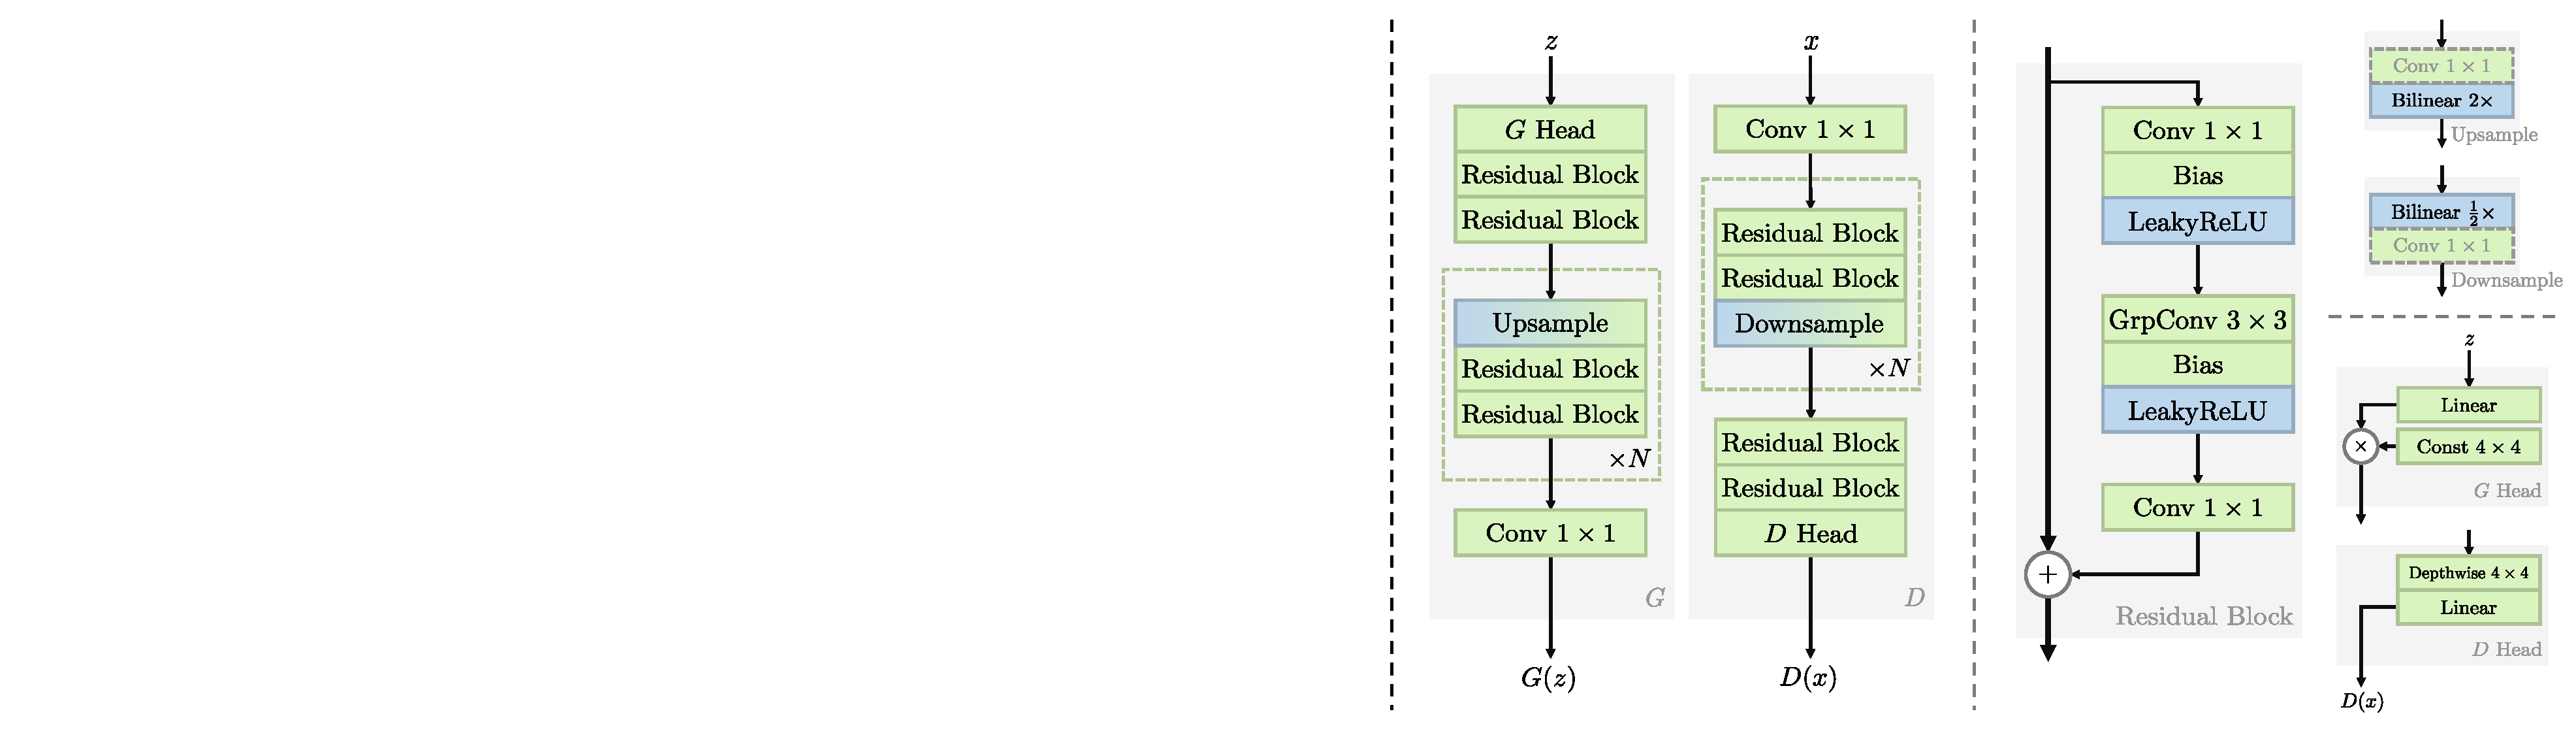
\includegraphics[width=\linewidth,clip,trim={87pc 0cm 0cm 0cm}]{figures/network.pdf}
    \caption{Network architecture blocks.}
    \label{fig:network}
    \vspace{-0.7cm}
\end{figure}

\paragraph{Bottleneck modernization (Config E).}
Now that we have settled on the overall architecture, we investigate how the residual block can be modernized, specifically i.\ref{item:i1}) and i.\ref{item:i2}). First, we explore i.\ref{item:i1} and replace the $3\times3$ convolution in the residual block with a grouped convolution. We set the group size to 16 rather than 1 (\ie depthwise convolution as in ConvNeXt) as depthwise convolution is highly inefficient on GPUs and is not much faster than using a larger group size. With grouped convolution, we can reduce the bottleneck compression ratio to two given the same model size. This increases the width of the bottleneck to $1.5\times$ as wide as Config A. 
%With this, the FID drops to 7.51, surpassing the performance of StyleGAN2. 
Finally, we notice that the compute cost of grouped convolution is negligible compared to $1\times1$ convolution, and so we seek to enhance the capacity of grouped convolution. We apply i.\ref{item:i2}), which inverts the bottleneck width and the stem width, and which doubles the width of grouped convolutions without any increase in model size. Figure~\ref{fig:network} depicts our final design, which reflects modern CNN architectures.

\section{Experiments}
\label{sec:exp}
We evaluate our model on FFHQ ($256\times256$)~\cite{sg1} for high resolution unimodal image synthesis, and high diversity generation on CIFAR-10~\cite{krizhevsky2009learning}, and ImageNet ($32\times32$)~\cite{chrabaszcz2017downsampled}. We compare our model with various baselines, in Table \ref{tab:ffhq256}, \ref{tab:cifar10}, and \ref{tab:imagenet32}.

We leave a detailed discussion of our results in Appendix E. Our model surpasses StyleGAN2 and StyleGAN3 by a large margin across datasets despite its simplicity. Unless with ImageNet feature leakage~\cite{sauer2021projected,kynkaanniemi2022role} or certain regularization~\cite{zhao2021improved} that has been shown to overfit~\cite{zhang2022styleswin} on FFHQ $256\times256$, no GAN comes close to R3GAN in terms of FID. Our model also beats diffusion models despite having a considerably smaller model size and that it generates samples in one step.\looseness=-1 








\vspace{-2ex}

\begin{table}[]
        \begin{tblr}{
          column{2} = {r},
          cell{1}{2} = {c},
          hline{2,5,9,10} = {-}{},
        }
        Model       & FID$\downarrow$  \\
        StyleGAN2   & 3.78 \\
        StyleGAN3-T & 4.81 \\
        StyleGAN3-R & 3.92 \\
        LDM & 4.98\\
        ADM (DDIM) & 8.41\\
        ADM (DPM-Solver) & 8.40\\
        Diffusion Autoencoder & 5.81\\
        Ours---Config E  & 2.77 \\
        \emph{With ImageNet feature leakage~\cite{kynkaanniemi2022role}:} & \\
        PolyINR*~\cite{singh2023polynomial} & 2.72 \\
        StyleGAN-XL*~\cite{sgxl} & 2.19 \\
        StyleSAN-XL*~\cite{takida2024san} & 1.36 \\
        \end{tblr}
        \caption{
        \label{tab:ffhq256}FFHQ-256. * denotes models that leak ImageNet features.}
        \vspace{-0.7cm}
\end{table}

\begin{table}[]
        \vspace{-0.2cm}
        \begin{tblr}{
          column{2} = {r},
          cell{1}{2}{3} = {},
          hline{2,9,13} = {-}{},
        }
        Model               & FID$\downarrow$ \\
        BigGAN~\cite{biggan}              & 14.73 \\
        TransGAN~\cite{trans}            & 9.26 \\
        ViTGAN~\cite{vitgan}              & 6.66 \\
        DDGAN~\cite{ddgan}               & 3.75 \\
        Diffusion StyleGAN2 & 3.19 \\
        StyleGAN2 + ADA     & 2.42 \\
        StyleGAN3-R + ADA   & 10.83 \\
        DDPM               & 3.21 \\
        DDIM                & 4.67 \\
        VE~\cite{edm}                  & 3.11 \\
        VP~\cite{edm}                  & 2.48 \\
        Ours---Config E     & 1.97 \\
        \hline
        \emph{With ImageNet feature leakage~\cite{kynkaanniemi2022role}:} & \\
        StyleGAN-XL*~\cite{sgxl}       & 	1.85 \\
        \end{tblr}
        \caption{\label{tab:cifar10}CIFAR-10.}
        %\vspace{-0.7cm}
\end{table}
\begin{table}[h!]
        \begin{tblr}{
          column{2} = {r},
          cell{1}{2} = {c},
          hline{2,5,9,10} = {-}{},
        }
        Model               & FID$\downarrow$       \\
        \emph{Unconditional} & \\
        DDPM++~\cite{kim2021soft}           & 8.42  \\ % (is unconditional)
        VDM~\cite{kingma2021variational}    & 7.41  \\ % (is unconditional)
        \emph{Conditional} & \\
        MSGAN~\cite{karnewar2020msg}        & 12.3  \\
        ADM~\cite{adm,ning2023input}                      & 3.60  \\
        DDPM-IP~\cite{ning2023input}        & 2.87  \\
        Ours---Config E                     & 1.27  \\ 
        \emph{With ImageNet feature leakage~\cite{kynkaanniemi2022role}:} & \\
        StyleGAN-XL*~\cite{sgxl}            & 1.10  \\
        \end{tblr}
        \caption{\label{tab:imagenet32}ImageNet-32.}
        %\vspace{-0.7cm}
\end{table}
\clearpage
{\small
\bibliographystyle{ieee_fullname}
\bibliography{bib/face_editing}
}

\appendix
\clearpage
\section*{Appendices}

\section{A Practical Demonstration of Our Loss.}
%\vk{i don't think that the rest of this section belongs in the methods section; i would first make it less verbose, then i would move large parts of it to the experiments, and i would summarize here in 1-2 sentences} 

We experiment with how well-behaved our loss is on StackedMNIST~\cite{pacgan} which consists of 1000 uniformly-distributed modes. The network is a small ResNet~\cite{resnet2} for $G$ and $D$ without any normalization layers~\cite{bn,gn,ln,in}.
Through the use of a pretrained MNIST classifier, we can explicitly measure how many modes of $p_\mathcal{D}$ are recovered by $p_\theta$. Furthermore, we can estimate the reverse KL divergence between the fake and real samples $D_\text{KL}\left(p_\theta\parallel p_\mathcal{D} \right)$ via the KL divergence between the categorical distribution of $p_\theta$ and the true uniform distribution.
\begin{figure}[t]
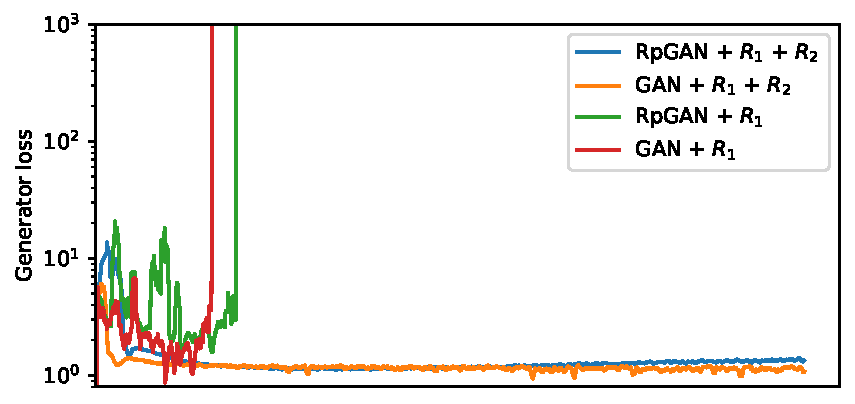
\includegraphics[width=1\linewidth]{figures/MNIST_loss.pdf}
\caption{Generator $G$ loss for different objectives over training. Regardless of which objective is used, training diverges with only $R_1$ and succeeded with both $R_1$ and $R_2$. Convergence failure with only $R_1$ was noted by Lee et al.~\cite{vitgan}.}
\label{fig:mnist_loss_curve}
\end{figure}

%For our initial experiments, we adopt a small ResNet~\cite{resnet2} architecture without any normalization layer~\cite{bn,gn,ln,in} for $G$ and $D$. 
A conventional GAN loss with $R_1$, as used by Mescheder et al.~\cite{r1} and the StyleGAN series~\cite{sg1, sg2, sg3}, diverges quickly (Fig.~\ref{fig:mnist_loss_curve}). Next, while theoretically sufficient for local convergence, RpGAN with only $R_1$ regularization is also unstable and diverges quickly\footnote{Varying $\gamma$ from 0.1 to 100 does not stabilize training.}. In each case, the gradient of $D$ on fake samples explodes when training diverges. With both $R_1$ and $R_2$, training becomes stable for both the classic GAN and RpGAN. Now stable, we can see that the classic GAN suffers from mode dropping, whereas RpGAN achieves full mode coverage (Table~\ref{tab:loss}) and reduces $D_\text{KL}$ from 0.9270 to 0.0781. As a point of contrast, StyleGAN~\cite{sg1,sg2,sg2ada,sg3} uses the minibatch standard deviation trick to reduce mode dropping, improving mode coverage from 857 to 881 on StackedMNIST and with barely any improvement on $D_\text{KL}$~\cite{pggan}.

%With training instability out of our way, we are ready to examine quantitatively how our new loss performs compared to existing work~\cite{r1,pggan,sg2}. While with $R_1$ and $R_2$ in conjunction training is successful for both the classic GAN~\cite{gan} and RpGAN~\cite{rgan}, we see in Table~\ref{tab:loss} that the classic GAN suffers from mode dropping. In contrast, RpGAN not only achieves full mode coverage, more notably, it drastically reduces $D_\text{KL}$ from 0.927 to 0.0781, indicating a considerably more faithful reconstruction of $p_\mathcal{D}$. 

% Instead of modifying the loss function, the StyleGAN family~\cite{sg1,sg2,sg2ada,sg3} relies on a trick called minibatch standard deviation~\cite{pggan} to combat mode dropping. It is shown in~\cite{pggan} that minibatch standard deviation can only slightly improve mode coverage from 857 to 881 on StackedMNIST and it shows barely any improvement on $D_\text{KL}$. 
% RpGAN in comparison improves mode coverage from 693 to 1000 and reduces $D_\text{KL}$ by one magnitude. 
%This shows that RpGAN is not only more principled against mode dropping in theory, but more effective in practice too. 
% We show in Section.\ref{sec:exp} that with architectural improvements in Section.\ref{sec:roadmap}, we can further improve $D_\text{KL}$ on StackedMNIST and even beat likelihood-based models. For the rest of this work, RpGAN $+ R_1+R_2$ will be our loss function.

% We start with RpGAN with only $R_1$ regularization since theoretically this is sufficient for local convergence. Contrary to our expectations, the training process utilizing this loss function exhibited significant instability and rapidly diverged. We experimented with various values of $\gamma$, ranging from 0.1 to 100; however, none succeeded in stabilizing the training. Furthermore, we explored integrating the conventional GAN loss combined with $R_1$, as commonly employed in the work of Mescheder et al.~\cite{r1} and the StyleGAN series~\cite{sg1, sg2, sg3}. Notably, this configuration led to even quicker divergence than the $R_1$ regularized RpGAN.
%To our surprise, training with this loss has been quite unstable and it diverges very quickly. We tried different $\gamma$ values ranging from 0.1 to 100 but none could prevent training from diverging. We also experiment with the combination of classic GAN and $R_1$, this is the widely adopted GAN loss in Mescheder~\etal~\cite{r1} and the StyleGAN family~\cite{sg1,sg2,sg3}, yet this loss diverges even faster than $R_1$ regularized RpGAN. 

% Upon closer inspection, we notice that the gradient of $D$ on fake samples explodes when training diverges. This motivates us to also apply $R_2$ regularization along with $R_1$, we see in Figure~\ref{fig:mnist_loss_curve} that with both $R_1$ and $R_2$, training becomes stable for both the classic GAN and RpGAN. 

\begin{table}[h]
\centering
    \begin{tabular}{ l rrr }
        \toprule
        Loss & \# modes$\uparrow$ & $D_\text{KL}$$\downarrow$ \\
        \midrule
        RpGAN $+ R_1+R_2$ & $\mathbf{1000}$ & $\mathbf{0.0781}$ \\
        GAN $+ R_1+R_2$ & $693$ & $0.9270$ \\
        RpGAN $+ R_1$ & Fail & Fail \\
        GAN $+ R_1$ & Fail & Fail \\
        \bottomrule
    \end{tabular}
    \caption{StackedMNIST~\cite{pacgan} result for each loss function. The maximum possible mode coverage is 1000. ``Fail'' indicates that training diverged early on.}
    \label{tab:loss}
\end{table}

$R_1$ alone is not sufficient for globally-convergent training. While a theoretical analysis of this is difficult, our small demonstration still provides insights into the assumptions of our convergence proof. 
In particular, the assumption that $(\theta,\psi)$ are sufficiently close to $(\theta^*,\psi^*)$ is highly unlikely early in training. In this scenario, if $D$ is sufficiently powerful, regularizing $D$ solely on real data is not likely to have much effect on $D$'s behavior on fake data and so training can fail due to an ill-behaved $D$ on fake data. 
% \vk{this is the key part that should be summarized in 1-2 sentences in this section: you find empirically and mathematically that both types of regularization are needed to make things work; then in the experiments section or in the appendix you provide results that show that it's the case}

Thus, the practical solution is to regularize $D$ on both real and fake data. The benefit of doing so can be viewed from the insight of Roth~\etal~\cite{r1r2}: that applying $R_1$ and $R_2$ in conjunction smooths both $p_\mathcal{D}$ and $p_\theta$ which makes learning easier than only smoothing $p_\mathcal{D}$. We also find empirically that with both $R_1$ and $R_2$ in place, $D$ tends to satisfy $\mathbb{E}_{x\sim p_\mathcal{D}}\left[\left\| \nabla_x D \right \|^2\right]\approx\mathbb{E}_{x\sim p_\theta}\left[\left\| \nabla_x D \right \|^2\right]$ even early in the training. Jolicoeur-Martineau~\etal~\cite{ganmmc} show that in this case $D$ becomes a maximum margin classifier---but if only one regularization term is applied, this does not hold.

% \vk{by the way, you will need a discussion of your regularization to other uses of this similar regularizer in the discussion or related work section}



\section{Experimental Findings from Config B.}
Violating \ref{item:convergent}, \ref{item:learning_rate}, or \ref{item:normalization} often leads to training failures.
%, contributing to the reputation that GANs as difficult to train. 
Gidel~\etal~\cite{ganmomentum} show that \emph{negative} momentum can improve GAN training dynamics. Since optimal negative momentum is another challenging hyperparameter, we do not use any momentum to avoid worsening GAN training dynamics. Studies~\cite{sg2,edm2} suggest normalization layers harm generative models. Batch normalization~\cite{bn} often cripples training due to dependencies across multiple samples, and is incompatible with $R_1$, $R_2$, or RpGAN that assume independent handling of each sample. Weaker data-independent normalizations~\cite{sg2,edm2} might help; we leave this for future work. Early GANs may succeed despite violating \ref{item:convergent} and \ref{item:normalization}, possibly constituting a full-rank solution~\cite{r1} to Eq.~\ref{eq:gan}.

Violations of \ref{item:resampling} or \ref{item:activation} do not significantly impair training stability but negatively affect sample quality. Improper transposed convolution can cause checkerboard artifacts, unresolved even with subpixel convolution~\cite{subpixel} or carefully tuned transposed convolution unless a low-pass filter is applied. Interpolation methods avoid this issue, varying from nearest neighbor~\cite{pggan} to Kaiser filters~\cite{sg3}. We use bilinear interpolation for simplicity. For activation functions, smooth approximations of (leaky) ReLU, such as Swish~\cite{swish}, GELU~\cite{gelu}, and SMU~\cite{smu}, worsen FID. PReLU~\cite{prelu} marginally improves FID but increases VRAM usage, so we use leaky ReLU.

All subsequent configurations adhere to \ref{item:convergent} through \ref{item:activation}. Violation of \ref{item:input} is acceptable as it pertains to the network backbone of StyleGAN2~\cite{sg2}, modernized in Config D and E.


\section{Network Architecture Details of Config D}
\vspace{-0.5ex}
Given i.\ref{item:i3}, i.\ref{item:i4}, and principles c), d), and e), we can replace the StyleGAN2 backbone with a modernized ResNet. We use a fully symmetric design for $G$ and $D$ with 25M parameters each, comparable to Config-A. The architecture is minimalist: each resolution stage has one transition layer and two residual blocks. The transition layer consists of bilinear resampling and an optional $1\times1$ conv for changing spatial size and feature map channels. The residual block includes five operations: Conv$1\times1\rightarrow$ Leaky ReLU $\rightarrow$ Conv$3\times3\rightarrow$ Leaky ReLU $\rightarrow$ Conv$1\times1$, with the final Conv$1\times1$ having no bias term. For the $4\times4$ resolution stage, the transition layer is replaced by a basis layer for $G$ and a classifier head for $D$. The basis layer, similar to StyleGAN~\cite{sg1,sg2}, uses $4\times4$ learnable feature maps modulated by $z$ via a linear layer. The classifier head uses a global $4\times4$ depthwise conv.~to remove spatial extent, followed by a linear layer to produce $D$'s output. We maintain the width ratio for each resolution stage as in Config A, making the stem width $3\times$ as wide due to the efficient $1\times1$ conv. The $3\times3$ conv in the residual block has a compression ratio of 4, following~\cite{resnet,resnet2}, making the bottleneck width $0.75\times$ as wide as Config A.
%Given i.3), i.4) and principles c), d), and e), we are now ready to replace the StyleGAN2 backbone with a modernized ResNet. We adopt a fully symmetric design for $G$ and $D$, and make the model size comparable to Config A, both $G$ and $D$ have approximately 25M parameters. We keep the architecture as minimalist as possible, for each resolution stage, we have one transition layer and two residual blocks. The transition layer consists of bilinear resampling and an optional $1\times1$ conv that allows us to change the spatial size and the number of channels of the feature maps. The residual block contains five consecutive operations on the residual branch: Conv$1\times1\rightarrow$ Leaky ReLU $\rightarrow$ Conv$3\times3\rightarrow$ Leaky ReLU $\rightarrow$ Conv$1\times1$, and the final Conv$1\times1$ has no bias term. For the $4\times4$ resolution stage, the transition layer is replaced by a basis layer for $G$ and a classifier head for $D$. The basis layer resembles the const input of StyleGAN~\cite{sg1,sg2} where a set of $4\times4$ learnable feature maps are modulated by $z$ via a linear layer. The classifier head first removes the spatial extent of the feature maps with a global $4\times4$ depthwise conv; the features are then fed to a linear layer to produce the output of $D$. We keep the width ratio for each resolution stage the same as Config A, and we are able to make the stem width $3\times$ as wide as Config A given the same model size thanks to the more efficient $1\times1$ conv. The compression ratio for the $3\times3$ conv in the residual block is set to 4 following~\cite{resnet,resnet2}, this makes the bottleneck width $0.75\times$ as wide as Config A.

% The lack of normalization necessitates more careful initialization for ResNet to avoid variance explosion. We apply fix-up initialization~\cite{fixup} to our modernized networks to remedy this. Concretely, we zero-initialize the last conv layer in each residual block, and scale down the initialization of the other two conv layers in the residual block by $L^{-0.25}$ where $L$ is the number of residual blocks in the network. We do not employ any other trick from fixup~\cite{fixup} such as applying excessive bias terms and the use of a scalar multiplier. The new network architecture and the initialization scheme allow us to raise the learning rate to $1\times10^{-4}$ without encountering training instability.
To avoid variance explosion due to the lack of normalization, we employ fix-up initialization~\cite{fixup} for our modernized networks. Specifically, we zero-initialize the last convolutional layer in each residual block and scale down the initialization of the other two convolutional layers in the block by $L^{-0.25}$, where $L$ is the number of residual blocks. We avoid other fix-up tricks, such as excessive bias terms and a learnable multiplier.

% We show that removing all these architectural modifications of the original StyleGAN mildly harms performance, but not as much as one might expect in~\ref{sub:arc-experiments}. Furthermore, removing some components actually benefits FID.


% \begin{figure}
%     \centering
%     \includegraphics[width=0.25\linewidth]{example-image-a}

%     \caption{Swirl Figure. We show our model matches performance on Gaussian toy example. \aaron{Are we still doing a toy example}]}
%     \label{fig:enter-label}
% \end{figure}

% \begin{figure}
%     \centering
%     \includegraphics[width=0.25\linewidth]{example-image-b}
%     \caption{k-NN decision barrier. Intuitive example}
%     \label{fig:enter-label}
% \end{figure}
\vspace{-1ex}
\section{Roadmap Insights}
\vspace{-0.5ex}
\begin{table}[t]
\resizebox{1\linewidth}{!}{
\begin{tabular}{ l r c c c } 
\toprule
   & \multicolumn{1}{l}{Configuration}  & FID$\downarrow$                    & G \#params              & D \#params               \\ 
\midrule
A  & \multicolumn{1}{l}{StyleGAN2}  & 7.516                  & 24.767M                  & 24.001M                   \\
\midrule
B  & \multicolumn{1}{l}{Stripped StyleGAN2}                                                                                                                                                                                                                                                                                                                                                                                                                 &                        &                          &                           \\ 
   & \begin{tabular}[c]{@{}r@{}}\textcolor{red}{- $z$ normalization}\\ \textcolor{red}{- Minibatch stddev}\\ \textcolor{red}{- Equalized learning rate}\textcolor{red}{}\\\textcolor{red}{- Mapping network}\\ \textcolor{red}{- Style injection}\\ \textcolor{red}{- Weight mod / demod}\\ \textcolor{red}{- Noise injection}\\ \textcolor{red}{- Mixing regularization}\\ \textcolor{red}{- Path length regularization}\\ \textcolor{red}{- Lazy regularization}\textcolor{blue}{}\end{tabular} & \multirow{2}{*}{12.46} & \multirow{2}{*}{18.890M} & \multirow{2}{*}{23.996M}  \\ 
\midrule
C  & \multicolumn{1}{l}{Well-behaved Loss}                       &                        &                          &                           \\ 
 & \textcolor[rgb]{0,0.502,0.502}{+ RpGAN loss}                                                                                                                                                                                                                                                                                                                                                                                                                   & 11.77                                           & \multirow{2}{*}{18.890M} & \multirow{2}{*}{23.996M}                           \\ 
   & \textcolor[rgb]{0,0.502,0.502}{+ $R_2$ gradient penalty}                                                                                                                                                                                                                                                                                                                                                                                                & \multirow{1}{*}{11.65} &                          &                           \\ 
\midrule
D  & \multicolumn{1}{l}{ConvNeXt-ify pt.~1}                                                                                                                                                                                                                                                                                                                                                                                                                 &                        &                          &                           \\ 
 & \textcolor[rgb]{0,0.502,0.502}{+ ResNet-ify G $\&$ D}                                                                                                                                                                                                                                                                                                                                                                                                   & 10.17                  & 23.400M                  & \multirow{2}{*}{23.282M}  \\
   & \textcolor{red}{- Output skips}                                                                                                                                                                                                                                                                                                                                                                                                                         & 9.950 & 23.378M &                           \\ 
\midrule
E  & \multicolumn{1}{l}{ConvNeXt-ify pt.~2}                              &                        &                          &                           \\
 & \textcolor[rgb]{0,0.502,0.502}{+ ResNeXt-ify G $\&$ D}                                                                                                                                                                                                                                                                                                                                                                                                  & 7.507                  & 23.188M                  & 23.091M                   \\ 
   & \textcolor[rgb]{0,0.502,0.502}{+ Inverted bottleneck}                                                                                                                                         & 7.045 & 23.058M & 23.010M  \\ 
\bottomrule
\end{tabular}
}
\vspace{-0.25cm}
\caption{Model configuration performance and size.} 
\label{tab:roadmap}
\vspace{-1ex}
\end{table}

As per Table~\ref{tab:roadmap}, Config A (vanilla StyleGAN2) achieves an FID of 7.52 using the official implementation on FFHQ-256. Config B with all tricks removed achieves an FID of 12.46---performance drops as expected. 
Config C, with a well-behaved loss, achieves an FID of 11.65. But, now training is sufficiently stable to improve the architecture.

Config D, which improves $G$ and $D$ based on the classic ResNet and ConvNeXt findings, achieves an FID of 9.95. The output skips of the StyleGAN2 generator are no longer useful given our new architecture; including them produces a worse FID of 10.17. Karras~\etal find that the benefit of output skips is mostly related to gradient magnitude dynamics~\cite{sg3}, and this has been addressed by our ResNet architecture. For StyleGAN2, Karras~\etal conclude that a ResNet architecture is harmful to $G$~\cite{sg2}, but this is not true in our case as their ResNet implementation is considerably different from ours: 1) Karras~\etal use one 3-3 residual block for each resolution stage, while we have a separate transition layer and two 1-3-1 residual blocks; 2) i.3) and i.4) are violated as they do not have a linear residual block~\cite{mobnet} and the transition layer is placed on the skip branch of the residual block rather than the stem; 3) the essential principle of ResNet~\cite{resnet}---identity mapping~\cite{resnet2}---is violated as Karras~\etal divide the output of the residual block by $\sqrt{2}$ to avoid variance explosion due to the absence of a proper initialization scheme.

For Config E, we conduct two experiments that ablate i.\ref{item:i1} (increased width with depthwise conv.) and i.\ref{item:i2} (an inverted bottleneck). We add GroupedConv and reduce the bottleneck compression ratio to two given the same model size. Each bottleneck is now 1.5$\times$ the width of Config A, and the FID drops to 7.51, surpassing the performance of StyleGAN2. By inverting the stem and the bottleneck dimensions to enhance the capacity of GroupedConv, our final model achieves an FID of 7.05, exceeding StyleGAN2.

\section{Experiments Details}
\begin{table}[]
\begin{tblr}{
  cell{2}{2} = {c},
  cell{2}{3} = {c},
  cell{3}{2} = {c},
  cell{3}{3} = {c},
  cell{4}{2} = {c},
  cell{4}{3} = {c},
  cell{5}{2} = {c},
  cell{5}{3} = {c},
  cell{6}{2} = {c},
  cell{6}{3} = {c},
  cell{7}{2} = {c},
  cell{7}{3} = {c},
  cell{8}{2} = {c},
  cell{8}{3} = {c},
  cell{9}{2} = {c},
  cell{9}{3} = {c},
  cell{10}{2} = {c},
  cell{10}{3} = {c},
  cell{11}{2} = {c},
  cell{11}{3} = {c},
  cell{12}{2} = {c},
  cell{12}{3} = {c},
  hline{2,12} = {1-3}{},
}
Model     & \# modes$\uparrow$ & $D_\text{KL}$$\downarrow$            &  \\
DCGAN~\cite{dcgan}     & 99            & 3.40\phantom{0}&  \\
VEEGAN~\cite{srivastava2017veegan}    & 150           & 2.95\phantom{0}&  \\
WGAN-GP~\cite{wgan-gp}& 959           & 0.73\phantom{0}&  \\
PacGAN~\cite{pacgan}    & 992           & 0.28\phantom{0}&  \\
StyleGAN2~\cite{sg2} & 940           & 0.42\phantom{0}&  \\
PresGAN~\cite{presgan}   & \textbf{1000} & 0.12\phantom{0}&  \\
Adv. DSM~\cite{advsm}  & \textbf{1000} & 1.49\phantom{0}&  \\
VAEBM~\cite{vaebm}     & \textbf{1000} & 0.087          &  \\
DDGAN~\cite{ddgan}     & \textbf{1000} & 0.071          &  \\
MEG~\cite{meg}       & \textbf{1000} & 0.031          &  \\
Ours---Config E     & \textbf{1000} & \textbf{0.029} &  
\end{tblr}
\caption{StackedMNIST 1000-mode coverage.}
\label{tab:stackedmnist}
\end{table}





\subsection{Mode recovery --- StackedMNIST\texorpdfstring{~\cite{metz2016unrolled}}{}} 
\vspace{-0.1cm}
We repeat the earlier experiment in 1000-mode convergence on StackedMNIST (unconditional generation), but this time with our updated architecture and with comparisons to SOTA GANs and likelihood-based methods (Tab.~\ref{tab:stackedmnist}, Fig.~\ref{fig:stacked-mnist}). 
One advantage brought up of likelihood-based models such as diffusion over GANs is that they achieve mode coverage~\cite{adm}. We find that most GANs struggle to find all modes. But, PresGAN~\cite{presgan}, DDGAN~\cite{ddgan} and our approach are successful. Further, our method outperforms all other tested GAN models in term of KL divergence.

\subsection{FID --- FFHQ-256\texorpdfstring{~\cite{sg1}}{} (Optimized)}
\vspace{-0.1cm}
We train Config E model until convergence and with optimized hyperparameters and training schedule on FFHQ at $256 \times 256$ (unconditional generation) (Tab.~\ref{tab:ffhq256}, Figs.~\ref{fig:ffhq-256-teaser} and~\ref{fig:ffhq-256}). The hyperparameters and schedule are listed in Appendix J. We outperform existing StyleGAN methods, plus four more recent diffusion-based methods. This particular dataset experimental setting is so common that many methods (not listed here) use the bCR~\cite{zhao2021improved} trick---this has only been shown to improve performance on FFHQ-256 (not even at different resolutions of FFHQ)~\cite{zhao2021improved, zhang2022styleswin}. We use no such tricks in our method.
% to achieve this performance.

\begin{figure}[h!]
    \newlength{\imgsize}
    \setlength{\imgsize}{0.10\linewidth} % Adjust this value to change the size of the images
    
    % New command to include images from a specific directory
    \newcommand{\qualitativeimg}[1]{%
        \includegraphics[width=\imgsize]{figures/qualitative/ffhq-256-000139623/image-#1.jpg}%
    }
    
    \setlength{\tabcolsep}{0pt} % Remove spacing between columns
    \renewcommand{\arraystretch}{0} % Remove spacing between rows
    
    \centering
    \begin{tabular}{cccccccc} % Eight columns
        \qualitativeimg{64} & \qualitativeimg{65} & \qualitativeimg{66} & \qualitativeimg{67} & \qualitativeimg{128} & \qualitativeimg{69} & \qualitativeimg{70} & \qualitativeimg{71} \\
        \qualitativeimg{72} & \qualitativeimg{73} & \qualitativeimg{74} & \qualitativeimg{75} & \qualitativeimg{76} & \qualitativeimg{77} & \qualitativeimg{78} & \qualitativeimg{79} \\
        \qualitativeimg{80} & \qualitativeimg{81} & \qualitativeimg{82} & \qualitativeimg{83} & \qualitativeimg{84} & \qualitativeimg{85} & \qualitativeimg{86} & \qualitativeimg{87} \\
        \qualitativeimg{88} & \qualitativeimg{89} & \qualitativeimg{90} & \qualitativeimg{91} & \qualitativeimg{92} & \qualitativeimg{93} & \qualitativeimg{94} & \qualitativeimg{95} \\
        \qualitativeimg{96} & \qualitativeimg{97} & \qualitativeimg{98} & \qualitativeimg{99} & \qualitativeimg{100} & \qualitativeimg{101} & \qualitativeimg{102} & \qualitativeimg{103} \\
        \qualitativeimg{104} & \qualitativeimg{105} & \qualitativeimg{106} & \qualitativeimg{107} & \qualitativeimg{108} & \qualitativeimg{109} & \qualitativeimg{110} & \qualitativeimg{111} \\
        \qualitativeimg{112} & \qualitativeimg{113} & \qualitativeimg{114} & \qualitativeimg{115} & \qualitativeimg{116} & \qualitativeimg{117} & \qualitativeimg{118} & \qualitativeimg{119} \\
        \qualitativeimg{120} & \qualitativeimg{121} & \qualitativeimg{122} & \qualitativeimg{123} & \qualitativeimg{124} & \qualitativeimg{125} & \qualitativeimg{126} & \qualitativeimg{127} \\
    \end{tabular}
    \caption{Qualitative examples of sample generation from our Config E on FFHQ-256.}
    \label{fig:ffhq-256-teaser}
\end{figure}


\subsection{FID --- CIFAR-10~\cite{krizhevsky2009learning}} \vspace{-0.1cm}
We train Config E model until convergence and with optimized hyperparameters and training schedule on CIFAR-10 (conditional generation) (Tab.~\ref{tab:cifar10}, Fig.~\ref{fig:cifar10}). Our method outperforms many other GANs by FID even though the model has relatively small capacity. For instance, StyleGAN-XL~\cite{sgxl} has 18\ M parameters in the generator and 125\ M parameters in the discriminator, while our model has a 40\ M parameters between the generator and discriminator combined (Fig.~\ref{fig:fid-50k-vs-params-cifar-10}). Compared to diffusion models like LDM or ADM, GAN inference is significantly cheaper as it requires only one network function evaluation compared to the tens or hundreds of network function evaluations for diffusion models without distillation. 

\begin{figure}[h]
    \centering
    % \includegraphics[width=\linewidth,clip,trim={0 0 0 2cm}]{figures/Scatterplot-FID-Parameters-CIFAR10.eps}
    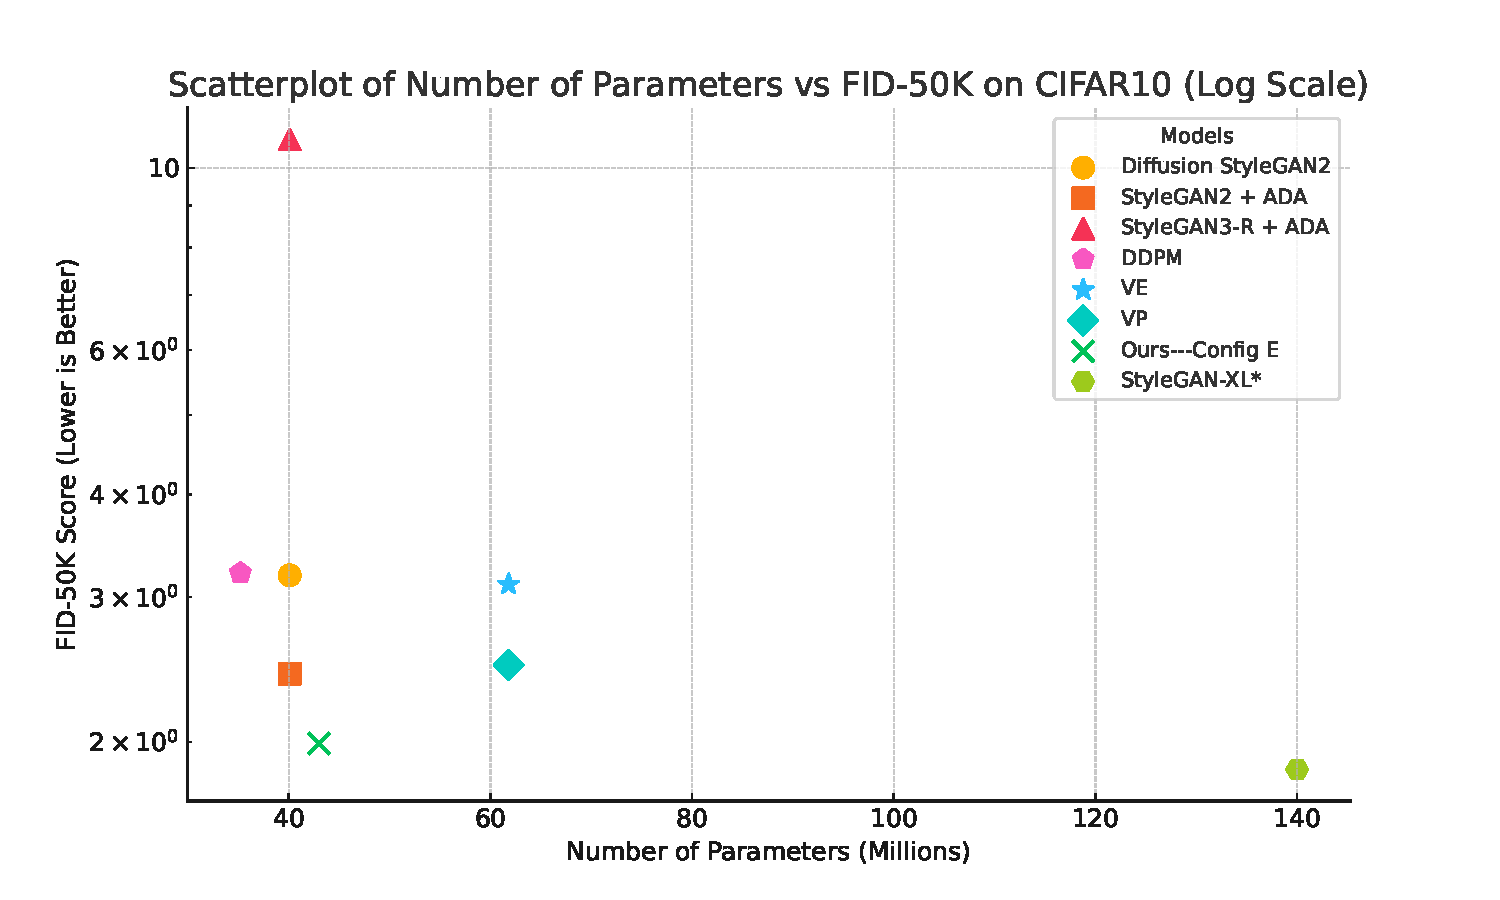
\includegraphics[width=\linewidth,clip,trim={0 0 0 2cm}]{figures/Scatterplot_FID_Parameters_CIFAR10_Log_Custom_Format.pdf}
    \caption{Number of parameters (millions) vs.~FID-50K (log scale) on CIFAR-10. Lower is better.}
    \label{fig:fid-50k-vs-params-cifar-10}
\end{figure}

Many state-of-the-art GANs are derived from Projected GAN~\cite{sauer2021projected}, including StyleGAN-XL~\cite{sgxl} and the concurrent work of StyleSAN-XL~\cite{takida2024san}. These methods use a pre-trained ImageNet classifier in the discriminator. Prior work has shown that a pre-trained ImageNet discriminator can leak ImageNet features into the model~\cite{kynkaanniemi2022role}, causing the model to perform better when evaluating on FID since it relies on a pre-trained ImageNet classifier for the loss. But, this does not improve results in perceptual studies~\cite{kynkaanniemi2022role}. Our model produces its low FID without any ImageNet pre-training.

\subsection{FID --- ImageNet-32~\cite{chrabaszcz2017downsampled}}

We train Config E model until convergence and with optimized hyperparameters and training schedule on ImageNet-32 (conditional generation). We compare against recent GAN models and recent diffusion models in Table~\ref{tab:imagenet32}.
We adjust the number of parameters in the generator of our model to match StyleGAN-XL~\cite{sgxl}'s generator (84 million parameters). Specifically, we make the model significantly wider to match. Our method achieves comparable FID despite using a 60\% smaller discriminator (Tab.~\ref{tab:imagenet32}) and despite not using a pre-trained ImageNet classifier.



\section{Discussion and Limitations}

We have shown that a simplication of GANs is possible for image generation tasks, built upon a more stable RpGAN$+ R_1 + R_2$ objective with mathematically-demonstrated convergence properties that still provides diverse output. This stability is what lets us re-engineer a modern network architecture without the tricks of previous methods, producing the \modelName model with competitive FID on the common datasets of Stacked-MNIST, FFHQ, CIFAR-10, and ImageNet-32 as an empirical demonstration of the mathematical benefits.

The focus of our work is to elucidate the essential components of a minimum GAN for image generation. 
As such, we prioritize simplicity over functionality---we do not claim to beat the performance of every existing model on every dataset or task; merely to provide a new simple baseline that converges easily.
While this makes our model an ideal backbone for future GANs, it also means that it is not suitable to apply our model directly to downstream applications such as image editing or controllable generation, as our model lacks dedicated features for easy image inversion or disentangled image synthesis. 
For instance, we remove style injection functionality from StyleGAN even though this has a clear use.
We also omitted common techniques that have been shown in previous literature to improve FID considerably. 
Examples include some form of adaptive normalization modulated by the latent code~\cite{adm,edm,sg1,zhang2022styleswin,dit}, and using multiheaded self attention at lower resolution stages~\cite{adm,edm,edm2}. 
We aim to explore these techniques in a subsequent study. 

Further, our work is limited in its evaluation of the scalability of \modelName models. While they show promising results on $32\times32$ ImageNet, we are yet to verify the scalability on higher resolution ImageNet data or large-scale text to image generation tasks.

Finally, as a method that can improve the quality of generative models, it would be amiss not to mention that generative models---especially of people---can cause direct harm (e.g., through personalized deep fakes) and societal harm through the spread of disinformation (e.g., fake influencers). 

\clearpage
\section{Local convergence}
Following~\cite{r1}, GAN training can be formulated as a dynamical system where the update operator is given by $F_h(\theta,\psi)=(\theta,\psi)+hv(\theta,\psi)$. $h$ is the learning rate and $v$ denotes the gradient vector field:
\begin{equation}
v(\theta,\psi)=\begin{pmatrix}
 -\nabla_\theta\mathcal{L}(\theta,\psi) \\
 \nabla_\psi\mathcal{L}(\theta,\psi)
\end{pmatrix}
\end{equation}
Mescheder et al.~\cite{gannum} showed that local convergence near $(\theta^*,\psi^*)$ can be analyzed by examining the spectrum of the Jacobian $\textbf{J}_{F_h}$ at the equilibrium: if the Jacobian has eigenvalues with absolute value bigger than 1, then training does not converge. On the other hand, if all eigenvalues have absolute value smaller than 1, then training will converge to $(\theta^*,\psi^*)$ at a linear rate. If all eigenvalues have absolute value equal to 1, the convergence behavior is undetermined.

Given some calculations~\cite{r1}, we can show that the eigenvalues of the Jacobian of the update operator $\lambda_{\textbf{J}_{F_h}}$ can be determined by $\lambda_{\textbf{J}_v}$:
\begin{equation}
\lambda_{\textbf{J}_{F_h}}=1+h\lambda_{\textbf{J}_v}\ .
\end{equation}
That is, given small enough $h$~\cite{r1}, the training dynamics can instead be examined using $\lambda_{\textbf{J}_v}$,~\ie, the eigenvalues of the Jacobian of the gradient vector field. If all $\lambda_{\textbf{J}_v}$ have a negative real part, the training will locally converge to $(\theta^*,\psi^*)$ at a linear rate. On the other hand, if some $\lambda_{\textbf{J}_v}$ have a positive real part, the training is not convergent. If all $\lambda_{\textbf{J}_v}$ have a zero real part, the convergence behavior is inconclusive.

\section{DiracRpGAN: A demonstration of non-convergence}
\paragraph{Summary.} To obtain DiracRpGAN, we apply Eq.~\ref{eq:rpgan} to the DiracGAN~\cite{r1} problem setting. After simplification, DiracRpGAN and DiracGAN are different only by a constant. They have the same gradient vector field, therefore all proofs are identical to Mescheder~\etal~\cite{r1}.

\paragraph{Definition B.1.} \emph{The DiracRpGAN consists of a (univariate) generator distribution $p_{\theta} = \delta_{\theta}$ and a linear discriminator $D_{\psi}(x) = \psi \cdot x$. The true data distribution $p_{\mathcal{D}}$ is given by a Dirac distribution concentrated at 0.}

In this setup, the RpGAN training objective is given by:
\begin{equation}
\label{eq:diracrpgan}
    \mathcal{L}(\theta, \psi) = f(\psi \theta)\ .
\end{equation}
We can now show analytically that DiracRpGAN does not converge without regularzation.

\paragraph{Lemma B.2.} \emph{The unique equilibrium point of the training objective in Eq.~\ref{eq:diracrpgan} is given by $\theta = \psi = 0$. Moreover, the Jacobian of the gradient vector field at the equilibrium point has the two eigenvalues $\pm f'(0)i$ which are both on the imaginary axis.}

The gradient vector field $v$ of Eq.~\ref{eq:diracrpgan} is given by:
\begin{equation}
    v(\theta, \psi) =
    \begin{pmatrix}
    -\nabla_{\theta} \mathcal{L}(\theta, \psi) \\
    \nabla_{\psi} \mathcal{L}(\theta, \psi)
    \end{pmatrix} =
    \begin{pmatrix}
    -\psi f'(\psi \theta) \\
    \theta f'(\psi \theta)
    \end{pmatrix}
\end{equation}
and the Jacobian of $v$:
\begin{equation}
    \textbf{J}_v =
    \begin{pmatrix}
    -\psi^2 f''(\psi\theta) & -f'(\psi\theta) - \psi\theta f''(\psi\theta) \\
    f'(\psi\theta) + \psi\theta f''(\psi\theta) & \theta^2 f''(\psi\theta)
    \end{pmatrix}
\end{equation}
Evaluating $\textbf{J}_v$ at the equilibrium point $\theta = \psi = 0$ gives us:
\begin{equation}
    \textbf{J}_v \biggr\rvert_{(0,0)} =
    \begin{pmatrix}
    0 & -f'(0) \\
    f'(0) & 0
    \end{pmatrix}
\end{equation}
Therefore, the eigenvalues of $\textbf{J}_v$ are $\lambda_{1/2} = \pm f'(0) i$, both of which have a real part of 0. Thus, the convergence of DiracRpGAN is inconclusive and further analysis is required.

\paragraph{Lemma B.3.} \emph{The integral curves of the gradient vector field $v(\theta, \psi)$ do not converge to the equilibrium point. More specifically, every integral curve $(\theta(t), \psi(t))$ of the gradient vector field $v(\theta, \psi)$ satisfies $\theta(t)^2 + \psi(t)^2 = const$ for all $t \in [0, \infty)$.}

Let $R(\theta, \psi) = \frac{1}{2} (\theta^2 + \psi^2)$, then:
\begin{align}
    & \frac{\mathrm{d}}{\mathrm{d}t} R(\theta(t), \psi(t)) \nonumber \\
    &= -\theta(t) \psi(t) f'(\theta(t) \psi(t)) + \psi(t) \theta(t) f'(\theta(t) \psi(t)) \nonumber \\
    &= 0\ .
\end{align}
We see that the distance between $(\theta, \psi)$ and the equilibrium point $(0,0)$ stays constant. Therefore, training runs in circles and never converges.

Next, we investigate the convergence behavior of DiracRpGAN with regularization. For DiracRpGAN, both $R_1$ and $R_2$ can be reduced to the following form:
\begin{equation}
    R(\psi) = \frac{\gamma}{2} \psi^2
\end{equation}

\paragraph{Lemma B.4.} \emph{The eigenvalues of the Jacobian of the gradient vector field for the gradient-regularized DiracRpGAN at the equilibrium point are given by
\begin{equation}
\label{eq:ev}
    \lambda_{1/2} = -\frac{\gamma}{2} \pm \sqrt{\frac{\gamma^2}{4}-f'(0)}
\end{equation}
In particular, for $\gamma > 0$ all eigenvalues have a negative real part. Hence, gradient descent is locally convergent for small enough learning rates.}

With regularization, the gradient vector field becomes
\begin{equation}
    \Tilde{v} (\theta, \psi) =
    \begin{pmatrix}
        -\psi f'(\psi\theta) \\
        \theta f'(\psi\theta) - \gamma\psi
    \end{pmatrix}
\end{equation}
the Jacobian of $\Tilde{v}$ is then given by
\begin{equation}
    \textbf{J}_{\Tilde{v}} =
    \begin{pmatrix}
    -\psi^2 f''(\psi\theta) & -f'(\psi\theta) - \psi\theta f''(\psi\theta) \\
    f'(\psi\theta) + \psi\theta f''(\psi\theta) & \theta^2 f''(\psi\theta) - \gamma
    \end{pmatrix}
\end{equation}
evaluating the Jacobian at $\theta = \psi = 0$ yields
\begin{equation}
    \textbf{J}_{\Tilde{v}} \biggr\rvert_{(0, 0)} =
    \begin{pmatrix}
        0 & -f'(0) \\
        f'(0) & -\gamma
    \end{pmatrix}
\end{equation}
given some calculations, we arrive at Eq.\ref{eq:ev}.

\section{General Convergence Results}
\paragraph{Summary.} The proofs are largely the same as Mescheder~\etal~\cite{r1}. We use the same proving techniques, and only slightly modify the assumptions and proof details to adapt Mescheder~\etal's effort to RpGAN. Like in~\cite{r1}, our proofs do not rely on unrealistic assumptions such as $\supp p_\mathcal{D}=\supp p_\theta$.

\subsection{Assumptions}
We closely follow~\cite{r1} but modify the assumptions wherever necessary to tailor the proofs for RpGAN. Like in~\cite{r1}, we also consider the realizable case where there exists $\theta$ such that $G_\theta$ produces the true data distribution.

\paragraph{Assumption~\upperRomannumeral{1}.}
\label{a:1}
\emph{We have $p_{\theta^*}=p_\mathcal{D}$, and $D_{\psi^*}=C$ in some local neighborhood of $\supp p_\mathcal{D}$, where $C$ is some arbitrary constant.}

\noindent Since RpGAN is defined on critic difference rather than raw logits, we no longer require $D_{\psi^*}$ to produce 0 on $\supp p_\mathcal{D}$, instead any constant $C$ would suffice.

\paragraph{Assumption~\upperRomannumeral{2}.}
\label{a:2}
\emph{We have $f^\prime(0)\neq0$ and $f^{\prime\prime}(0)<0$.}

\noindent This assumption is the same as in~\cite{r1}. The choice $f(t) = -\log(1+e^{-t})$ adopted in the main text satisfies this assumption.

As discussed in~\cite{r1}, there generally is not a single equilibrium point $(\theta^*,\psi^*)$, but a submanifold of equivalent equilibria corresponding to different parameterizations of the same function. It is therefore necessary to represent the equilibrium as \emph{reparameterization manifolds} $\mathcal{M}_G$ and $\mathcal{M}_D$. We modify the reparameterization $h$ as follows:
\begin{equation}
\label{eq:h}
h(\psi)=\mathbb{E}_{\substack{x\sim p_\mathcal{D}\\y\sim p_\mathcal{D}}}\left[\left | D_\psi(x)-D_\psi(y)\right |^2   +  \left \| \nabla_x D_\psi(x) \right \|^2\right]
\end{equation}
to account for the fact that $D_{\psi^*}$ is now allowed to have any constant value on $\supp p_\mathcal{D}$. The \emph{reparameterization manifolds} are then given by:
\begin{align}
&\mathcal{M}_G=\{\theta\ \rvert\ p_\theta=p_\mathcal{D}\} \\
&\mathcal{M}_D=\{\psi\ \rvert\ h(\psi)=0 \}
\end{align}
We assume the same regularity properties as in~\cite{r1} for $\mathcal{M}_G$ and $\mathcal{M}_D$ near the equilibrium. To state these assumptions, we need:
\begin{equation}
g(\theta)=\mathbb{E}_{x\sim p_\theta}\left[\nabla_\psi D_\psi\rvert_{\psi=\psi^*}\right]
\end{equation}
which leads to:
\paragraph{Assumption~\upperRomannumeral{3}.}
\label{a:3}
\emph{There are $\epsilon$-balls $B_\epsilon(\theta^*)$ and $B_\epsilon(\psi^*)$ around $\theta^*$ and $\psi^*$ so that $\mathcal{M}_G\ \cap\ B_\epsilon(\theta^*)$ and $\mathcal{M}_D\ \cap\ B_\epsilon(\psi^*)$ define $\mathcal{C}^1$-manifolds. Moreover, the following holds}:
\begin{enumerate}[label=(\roman*)]
\item \emph{if $v\in\mathbb{R}^n$ is not in $\mathcal{T}_{\psi^*}\mathcal{M}_D$, then $\partial_v^2h(\psi^*)\neq0$}.
\item \emph{if $w\in\mathbb{R}^m$ is not in $\mathcal{T}_{\theta^*}\mathcal{M}_G$, then $\partial_wg(\theta^*)\neq0$}.
\end{enumerate}

These two conditions have exactly the same meanings as in~\cite{r1}: the first condition indicates the geometry of $\mathcal{M}_D$ can be locally described by the second derivative of $h$. The second condition implies that $D$ is strong enough that it can detect any deviation from the equilibrium generator distribution. This is the only assumption we have about the expressiveness of $D$.

\subsection{Convergence}
We can now show the general convergence result for gradient penalized RpGAN, consider the gradient vector field with either $R_1$ or $R_2$ regularization:
\begin{equation}
\label{eq:vreg}
\tilde{v}_i(\theta,\psi)=\begin{pmatrix}
-\nabla_\theta\mathcal{L}(\theta,\psi)\\ 
\nabla_\psi\mathcal{L}(\theta,\psi)-\nabla_\psi R_i(\theta,\psi)
\end{pmatrix}
\end{equation}
note that the convergence result can also be trivially extended to the case where both $R_1$ and $R_2$ are applied. We omit the proof for this case as it is redundant once the convergence with either regularization is proven.

\paragraph{Theorem.} \emph{Assume Assumption~\upperRomannumeral{1},~\upperRomannumeral{2} and~~\upperRomannumeral{3} hold for $(\theta^*,\psi^*)$. For small enough learning rates, gradient descent for $\tilde{v}_1$ and $\tilde{v}_2$ are both convergent to $\mathcal{M}_G\times\mathcal{M}_D$ in a neighborhood of $(\theta^*,\psi^*)$. Moreover, the rate of convergence is at least linear}.

We extend the convergence proof by Mescheder~\etal~\cite{r1} to our setting. We first prove lemmas necessary to our main proof.

\paragraph{Lemma C.2.1.} \emph{Assume $J\in\mathbb{R}^{(n+m)\times(n+m)}$ is of the following form}:
\begin{equation}
J=\begin{pmatrix}
0 & -B^\top\\ 
B & -Q
\end{pmatrix}
\end{equation}
\emph{where $Q\in\mathbb{R}^{m\times m}$ is a symmetric positive definite matrix and $B\in\mathbb{R}^{m\times n}$ has full column rank. Then all eigenvalues $\lambda$ of $J$ satisfy $\Re(\lambda)< 0$}.

\emph{Proof.} See Mescheder~\etal~\cite{r1}, Theorem A.7.

\paragraph{Lemma C.2.2.} \emph{The gradient of $\mathcal{L}(\theta,\psi)$~\wrt $\theta$ and $\psi$ are given by}:
\begin{align}
\nabla_\theta\mathcal{L}(\theta,\psi)=\mathbb{E}_{\substack{z\sim p_z\\x\sim p_\mathcal{D}}}[f^\prime(D_\psi(G_\theta(z))-D_\psi(x)) \nonumber \\ 
\left[\nabla_\theta G_\theta(z)\right]^\top\nabla_xD_\psi(G_\theta(z))] \\
\label{grad_psi}
\nabla_\psi\mathcal{L}(\theta,\psi)=\mathbb{E}_{\substack{z\sim p_z\\x\sim p_\mathcal{D}}}[f^\prime(D_\psi(G_\theta(z))-D_\psi(x)) \nonumber \\
(\nabla_\psi D_\psi(G_\theta(z))-\nabla_\psi D_\psi(x))]
\end{align}
\emph{Proof.} This is just the chain rule.

\paragraph{Lemma C.2.3.} \emph{Assume that $(\theta^*,\psi^*)$ satisfies Assumption~\upperRomannumeral{1}. The Jacobian of the gradient vector field $v(\theta,\psi)$ at $(\theta^*,\psi^*)$ is then}
\begin{equation}
\textbf{J}_v\biggr\rvert_{(\theta^*,\psi^*)}=\begin{pmatrix}
0 & -K^\top_{DG}\\ 
K_{DG} & K_{DD}
\end{pmatrix}
\end{equation}
\emph{the terms $K_{DD}$ and $K_{DG}$ are given by}
\begin{align}
\label{kdd}
K_{DD}=f^{\prime\prime}(0)\mathbb{E}_{\substack{x\sim p_\mathcal{D}\\y\sim p_\mathcal{D}}}[(\nabla_\psi D_{\psi^*}(x)-\nabla_\psi D_{\psi^*}(y)) \nonumber \\
(\nabla_\psi D_{\psi^*}(x)-\nabla_\psi D_{\psi^*}(y))^\top] \\
\label{kdg}
K_{DG}=f^\prime(0)\nabla_\theta\mathbb{E}_{x\sim p_\theta}[\nabla_\psi D_{\psi^*}(x)]\ \rvert_{\theta=\theta^*}
\end{align}

\emph{Proof.} Note that
\begin{equation}
\textbf{J}_v\biggr\rvert_{(\theta^*,\psi^*)}=\begin{pmatrix}
-\nabla^2_\theta\mathcal{L}(\theta^*,\psi^*) & -\nabla^2_{\theta,\psi}\mathcal{L}(\theta^*,\psi^*) \\ 
\nabla^2_{\theta,\psi}\mathcal{L}(\theta^*,\psi^*) & \nabla^2_\psi\mathcal{L}(\theta^*,\psi^*)
\end{pmatrix}
\end{equation}
By Assumption~\upperRomannumeral{1}, $D_{\psi^*}=C$ in some neighborhood of $\supp p_\mathcal{D}$. Therefore we also have $\nabla_x D_{\psi^*}=0$ and $\nabla^2_x D_{\psi^*}=0$ for $x\in\supp p_\mathcal{D}$. Using these two conditions, we see that $\nabla^2_\theta\mathcal{L}(\theta^*,\psi^*)=0$.

To see Eq.\ref{kdd} and Eq.\ref{kdg}, simply take the derivatives of Eq.\ref{grad_psi} and evaluate at $(\theta^*,\psi^*)$.

\paragraph{Lemma C.2.4.} \emph{The gradient $\nabla_\psi R_i(\theta,\psi)$ of the regularization terms $R_i$, $i\in\{1,2\}$,~\wrt $\psi$ are}
\begin{align}
&\nabla_\psi R_1(\theta,\psi)=\gamma\mathbb{E}_{x\sim p_\mathcal{D}}[\nabla_{\psi,x}D_\psi\nabla_xD_\psi] \\
&\nabla_\psi R_2(\theta,\psi)=\gamma\mathbb{E}_{x\sim p_\theta}[\nabla_{\psi,x}D_\psi\nabla_xD_\psi]
\end{align}

\emph{Proof.} See Mescheder~\etal~\cite{r1}, Lemma D.3.

\paragraph{Lemma C.2.5.} \emph{The second derivatives $\nabla^2_\psi R_i(\theta^*,\psi^*)$ of the regularization terms $R_i$, $i\in\{1,2\}$,~\wrt $\psi$ at $(\theta^*,\psi^*)$ are both given by}
\begin{equation}
L_{DD}=\gamma\mathbb{E}_{x\sim p_\mathcal{D}}[AA^\top]
\end{equation}
\emph{where $A=\nabla_{\psi,x}D_{\psi^*}$. Moreover, both regularization terms satisfy $\nabla_{\theta,\psi}R_i(\theta^*,\psi^*)=0$.}

\emph{Proof.} See Mescheder~\etal~\cite{r1}, Lemma D.4.

Given Lemma C.2.3, Lemma C.2.5 and Eq.\ref{eq:vreg}, we can now show that the Jacobian of the regularized gradient field at the equilibrium point is given by
\begin{equation}
\textbf{J}_{\tilde{v}}\biggr\vert_{(\theta^*,\psi^*)}=\begin{pmatrix}
0 & -K_{DG}^\top\\ 
K_{DG} & M_{DD}
\end{pmatrix}
\end{equation}
where $M_{DD}=K_{DD}-L_{DD}$. To prove our main theorem, we need to examine $\textbf{J}_{\tilde{v}}$ when restricting it to the space orthogonal to $\mathcal{T}_{(\theta^*,\psi^*)}\mathcal{M}_G\times\mathcal{M}_D$.

\paragraph{Lemma C.2.6.} \emph{Assume Assumptions~\upperRomannumeral{2} and~\upperRomannumeral{3} hold. If $v\neq0$ is not in $\mathcal{T}_{\psi^*}\mathcal{M}_D$, then $v^\top M_{DD}v<0$.}

\emph{Proof.} By Lemma C.2.3 and Lemma C.2.5, we have
\begin{align}
\resizebox{0.42\textwidth}{!}{$
v^\top K_{DD}v=f^{\prime\prime}(0)\mathbb{E}_{\substack{x\sim p_\mathcal{D}\\y\sim p_\mathcal{D}}}\left[((\nabla_\psi D_{\psi^*}(x)-\nabla_\psi D_{\psi^*}(y))^\top v)^2\right]
$}
\end{align}
\begin{align}
v^\top L_{DD}v=\gamma\mathbb{E}_{x\sim p_\mathcal{D}}\left[\left\|Av\right \|^2\right]
\end{align}
By Assumption~\upperRomannumeral{2}, we have $f^{\prime\prime}(0)<0$. Therefore $v^\top M_{DD}v \leq 0$. Suppose $v^\top M_{DD}v=0$, this implies
\begin{equation}
(\nabla_\psi D_{\psi^*}(x)-\nabla_\psi D_{\psi^*}(y))^\top v=0\ \ \ \ \text{and}\ \ \ \ Av=0
\end{equation}
for all $(x,y)\in\supp\ p_\mathcal{D}\times\supp\ p_\mathcal{D}$. Recall the definition of $h(\psi)$ from Eq.\ref{eq:h}. Using the fact that $D_{\psi^*}=C$ and $\nabla_x D_{\psi^*}=0$ for $x\in\supp\ p_\mathcal{D}$, we see that the Hessian of $h(\psi)$ at $\psi^*$ is
\begin{align}
\nabla^2_\psi h(\psi^*)=2\mathbb{E}_{\substack{x\sim p_\mathcal{D}\\y\sim p_\mathcal{D}}}[(\nabla_\psi D_{\psi^*}(x)-\nabla_\psi D_{\psi^*}(y)) \nonumber \\
(\nabla_\psi D_{\psi^*}(x)-\nabla_\psi D_{\psi^*}(y))^\top+AA^\top]
\end{align}
The second directional derivative $\partial^2_v h(\psi)$ is therefore
\begin{align}
&\ \ \ \ \partial^2_v h(\psi) \nonumber \\
&=2\mathbb{E}_{\substack{x\sim p_\mathcal{D}\\y\sim p_\mathcal{D}}}\left[\left| (\nabla_\psi D_{\psi^*}(x)-\nabla_\psi D_{\psi^*}(y))^\top v\right|^2 + \left\|Av\right\|^2\right] \nonumber \\
&=0
\end{align}
By Assumption~\upperRomannumeral{3}, this can only hold if $v\in\mathcal{T}_{\psi^*}\mathcal{M}_D$.

\paragraph{Lemma C.2.7.} \emph{Assume Assumption~\upperRomannumeral{3} holds. If $w\neq0$ is not in $\mathcal{T}_{\theta^*}\mathcal{M}_G$, then $K_{DG}w\neq0$.}

\emph{Proof.} See Mescheder~\etal~\cite{r1}, Lemma D.6.

\emph{Proof for the main theorem.} Given previous lemmas, by choosing local coordinates $\theta(\alpha,\gamma_G)$ and $\psi(\beta,\gamma_D)$ for $\mathcal{M}_G$ and $\mathcal{M}_D$ such that $\theta^*=0$, $\psi^*=0$ as well as
\begin{align}
\mathcal{M}_G=\mathcal{T}_{\theta^*}\mathcal{M}_G=\{0\}^k\times\mathbb{R}^{n-k} \\
\mathcal{M}_D=\mathcal{T}_{\psi^*}\mathcal{M}_D=\{0\}^l\times\mathbb{R}^{m-l}
\end{align}
our proof is \emph{exactly} the same as Mescheder~\etal~\cite{r1}, Theorem 4.1.

\newpage
\section{Hyperparameters, training configurations, and compute}
We implement our models on top of the official StyleGAN3 code base. While the loss function and the models are implemented from scratch, we reuse support code from the existing implementation whenever possible. This includes exponential moving average (EMA) of generator weights~\cite{pggan}, non-leaky data augmentation~\cite{sg2ada}, and metric evaluation~\cite{sg3}.

\vspace{-0.1cm}
\paragraph{Training schedule.}
To speed up the convergence early in training, we specify a cosine schedule for the following hyperparameters before they reach their target values: 
\begin{itemize}[parsep=2pt,topsep=0pt,itemsep=0pt]
    \item Learning rate
    \item $\gamma$ for $R_1$ and $R_2$ regularization
    \item Adam $\beta_2$
    \item EMA half-life
    \item Augmentation probability
\end{itemize}
We call this early training stage the burn-in phase. Burn-in length and schedule for each hyperparameter are listed in Table~\ref{tab:hyperparam} for each experiment. A schedule for the EMA half-life can already be found in Karras~\etal~\cite{sg2ada}, albeit they use a linear schedule. A lower initial Adam $\beta_2$ is crucial to the initial large learning rate as it allows the optimizer to adapt to the gradient magnitude change much quicker. We use a large initial $\gamma$ to account for that early in training: $p_\theta$ and $p_\mathcal{D}$ are far apart and a large $\gamma$ smooths both distributions more aggressively which makes learning easier. Augmentation is not necessary until $D$ starts to overfit later on; thus, we set the initial augmentation probability to 0.

\vspace{-0.1cm}
\paragraph{Dataset augmentation.}
We apply horizontal flips and non-leaky augmentation~\cite{sg2ada} to all datasets where augmentation is enabled. Following~\cite{sg2ada}, we include pixel blitting, geometric transformations, and color transforms in the augmentation pipeline. We additionally include cutout augmentation which works particularly well with our model, although it does not seem to have much effect on StyleGAN2. We also find it beneficial to apply color transforms less often and thus set their probability multiplier to 0.5 while retaining the multiplier 1 for other types of augmentations. As previously mentioned, we apply a fixed cosine schedule to the augmentation probability rather than adjusting it adaptively as in~\cite{sg2ada}. We did not observe any performance degradation with this simplification.

\vspace{-0.1cm}
\paragraph{Network capacity.}
We keep the capacity distribution for each resolution the same as in~\cite{sg2ada,sg3}. We place two residual blocks per resolution which makes our model roughly $3\times$ as deep, $1.5\times\sim3\times$ as wide as StyleGAN2 while maintaining the same model size on CIFAR-10 and FFHQ. For the ImageNet model, we double the number of channels which results in roughly $4\times$ as many parameters as the default StyleGAN2 configuration.

\vspace{-0.1cm}
\paragraph{Mixed precision training.}
We apply mixed precision training as in~\cite{sg2ada,sg3} where all parameters are stored in FP32, but cast to lower precision along with the activation maps for the 4 highest resolutions. We notice that using FP16 as the low precision format cripples the training of our model. However, we see no problem when using BFloat16 instead.

\vspace{-0.1cm}
\paragraph{Class conditioning.}
For class conditional models, we follow the same conditioning scheme as in~\cite{sg2ada}. For $G$, the conditional latent code $z^\prime$ is the concatenation of $z$ and the embedding of the class label $c$, specifically $z^\prime=\text{concat}(z,\text{embed}(c))$. For $D$, we use a projection discriminator~\cite{cgans} which evaluates the dot product of the class embedding and the feature vector $D^\prime(x)$ produced by the last layer of $D$, concretely $D(x)=\text{embed}(c)\cdot D^\prime(x)^\top$. We do not employ any normalization-based conditioning such as AdaIN~\cite{sg1}, AdaGN~\cite{adm,edm}, AdaBN~\cite{biggan} or AdaLN~\cite{dit} for simplicity, even though they improve FID considerably.

\vspace{-0.1cm}
\paragraph{Stacked MNIST.}
We base this model off of the CIFAR-10 model but without class conditioning. We disable all data augmentation and shorten the burn-in phase considerably. We use a constant learning rate and did not observe any benefit of using a lower learning rate later in the training.

\vspace{-0.1cm}
\paragraph{Compute resources.}
We train the Stacked MNIST and CIFAR-10 models on an $8\times$ NVIDIA L40 node. Training took 7 hours for Stacked MNIST and 4 days for CIFAR-10. The FFHQ model was trained on an $8\times$ NVIDIA A6000 f0r roughly 3 weeks. The ImageNet model was trained on NVIDIA A100/H100 clusters and training took one day on 32 H100s (about 5000 H100 hours).

\begin{landscape}
\begin{table}[h]
\centering
\caption{\label{tab:hyperparam}Hyperparameters for each experiment. The decay factor $\beta$ of EMA can be obtained using the formula $\beta = 0.5^{\frac{\text{Minibatch size}}{\text{EMA half-life}}}$,~\eg for CIFAR-10, EMA $\beta=0.5^{\frac{512}{5\times10^6}}\approx0.9999$.}
\resizebox{\columnwidth}{!}{%
\begin{tblr}{
  column{even} = {c},
  column{3} = {c},
  column{5} = {c},
  column{7} = {c},
  cell{1}{4} = {c=2}{},
  cell{1}{6} = {c=2}{},
  hline{1-2,5,12,17,19} = {-}{},
}
Hyperparameter               & Stacked MNIST        & CIFAR-10                              & FFHQ                                  &                     & ImageNet                              &     \\
Resolution                   & $32\times32$         & $32\times32$                          & $256\times256$                        & $64\times64$                 & $32\times32$                          & $64\times64$ \\
Class conditional            & -                    & $\checkmark$                          & -                                     & -                   & $\checkmark$                          & $\checkmark$  \\
Number of GPUs               & 8                    & 8                                     & 8                                     & 8                   & 32                                    & 64 \\
Duration (Mimg)              & 10                   & 250                                   & 200                                   & 100                 & 1000                                   & 1000  \\
Burn-in (Mimg)               & 2                    & 20                                    & 20                                    & 20                  & 200                                   & 200  \\
Minibatch size               & 512                  & 512                                   & 256                                   & 256                 & 4096                                  & 4096  \\
Learning rate                & $2\times10^{-4}$       & $2\times10^{-4}\rightarrow5\times10^{-5}$ & $2\times10^{-4}\rightarrow5\times10^{-5}$ & $2\times10^{-4}\rightarrow5\times10^{-5}$                 & $2\times10^{-4}\rightarrow5\times10^{-5}$ & $2\times10^{-4}\rightarrow5\times10^{-5}$  \\
$\gamma$ for $R_1$ and $R_2$ & $1\rightarrow0.1$    & $0.05\rightarrow0.005$                & $150\rightarrow15$                    & $2\rightarrow0.2$                 & $0.5\rightarrow0.05$                  & $1\rightarrow0.1$  \\
Adam $\beta_2$               & $0.9\rightarrow0.99$ & $0.9\rightarrow0.99$                  & $0.9\rightarrow0.99$                  & $0.9\rightarrow0.99$                 & $0.9\rightarrow0.99$                  & $0.9\rightarrow0.99$  \\
EMA half-life (Mimg)         & $0\rightarrow0.5$    & $0\rightarrow5$                       & $0\rightarrow0.5$                     & $0\rightarrow0.5$                 & $0\rightarrow50$                      & $0\rightarrow50$  \\
Channels per resolution      & 768-768-768-768      & 768-768-768-768                       & 96-192-384-768-768-768-768            & 384-768-768-768-768 & 1536-1536-1536-1536                   & 1536-1536-1536-1536-1536  \\
ResBlocks per resolution     & 2-2-2-2              & 2-2-2-2                               & 2-2-2-2-2-2-2                         & 2-2-2-2-2                 & 2-2-2-2                               & 2-2-2-2-2  \\
Groups per resolution        & 96-96-96-96          & 96-96-96-96                           & 12-24-48-96-96-96-96                  & 48-96-96-96-96                 & 96-96-96-96                           & 96-96-96-96-96  \\
$G$~params                   & 20.73M               & 20.78M                                & 23.06M                                & 22.43M                 & 82.91M                                & 103.57M  \\
$D$~params                   & 20.68M               & 21.28M                                & 23.01M                                & 22.38M                 & 86.55M                                & 107.21M  \\
Dataset $x$-flips            & -                    & $\checkmark$                          & $\checkmark$                          & $\checkmark$                 & $\checkmark$                          & $\checkmark$  \\
Augment probability          & -                    & $0\rightarrow0.55$                    & $0\rightarrow0.3$                    & $0\rightarrow0.3$                 & $0\rightarrow0.5$                     & $0\rightarrow0.4$  
\end{tblr}
}
\end{table}
\end{landscape}



\section{Qualitative Results}
{
% Variable to control the size of each image
\begin{figure}[h!]
%    \newlength{\imgsize}
    \setlength{\imgsize}{\linewidth} % Adjust this value to change the size of the images
    
    \setlength{\tabcolsep}{0pt} % Remove spacing between columns
    \renewcommand{\arraystretch}{0} % Remove spacing between rows

    % New command to include images from a specific directory
    \newcommand{\qualitativeimg}[1]{%
        \includegraphics[width=\imgsize]{figures/qualitative/stacked-mnist-000008806/number-#1.jpg}%
    }
    \centering
    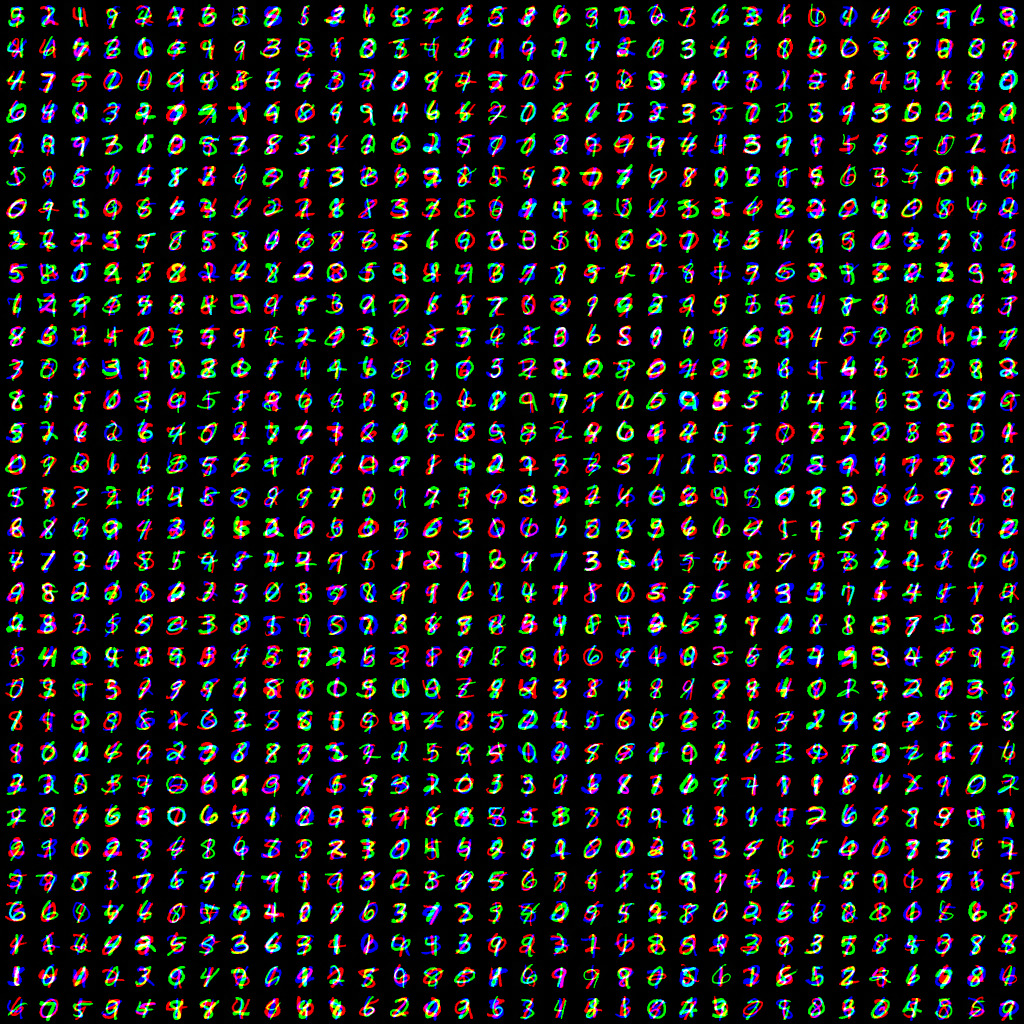
\includegraphics[width=\linewidth, clip, trim={0 0 768px 768px}]{figures/qualitative/stacked-mnist-000008806.jpg}
    \caption{Qualitative examples of sample generation from our Config E on Stacked-MNIST.}
    \label{fig:stacked-mnist}
\end{figure}
}
{
\begin{figure}[ht!]
    %\newlength{\imgsize}
    \setlength{\imgsize}{0.125\linewidth} % Adjust this value to change the size of the images
    
    % New command to include images from a specific directory
    \newcommand{\qualitativeimg}[1]{%
        \includegraphics[width=\imgsize]{figures/qualitative/ffhq-256-000139623/image-#1.jpg}%
    }
    
    \setlength{\tabcolsep}{0pt} % Remove spacing between columns
    \renewcommand{\arraystretch}{0} % Remove spacing between rows
    
    \centering
    \begin{tabular}{cccccccc} % Eight columns
        \qualitativeimg{0} & \qualitativeimg{1} & \qualitativeimg{2} & \qualitativeimg{3} & \qualitativeimg{4} & \qualitativeimg{5} & \qualitativeimg{6} & \qualitativeimg{7} \\
        \qualitativeimg{8} & \qualitativeimg{9} & \qualitativeimg{10} & \qualitativeimg{11} & \qualitativeimg{12} & \qualitativeimg{13} & \qualitativeimg{14} & \qualitativeimg{15} \\
        \qualitativeimg{16} & \qualitativeimg{17} & \qualitativeimg{18} & \qualitativeimg{19} & \qualitativeimg{20} & \qualitativeimg{71} & \qualitativeimg{22} & \qualitativeimg{23} \\
        \qualitativeimg{24} & \qualitativeimg{25} & \qualitativeimg{26} & \qualitativeimg{27} & \qualitativeimg{28} & \qualitativeimg{29} & \qualitativeimg{30} & \qualitativeimg{31} \\
        \qualitativeimg{32} & \qualitativeimg{33} & \qualitativeimg{34} & \qualitativeimg{35} & \qualitativeimg{36} & \qualitativeimg{37} & \qualitativeimg{38} & \qualitativeimg{39} \\
        \qualitativeimg{40} & \qualitativeimg{41} & \qualitativeimg{42} & \qualitativeimg{43} & \qualitativeimg{44} & \qualitativeimg{45} & \qualitativeimg{46} & \qualitativeimg{47} \\
        \qualitativeimg{48} & \qualitativeimg{49} & \qualitativeimg{50} & \qualitativeimg{51} & \qualitativeimg{52} & \qualitativeimg{53} & \qualitativeimg{54} & \qualitativeimg{55} \\
        \qualitativeimg{56} & \qualitativeimg{57} & \qualitativeimg{58} & \qualitativeimg{59} & \qualitativeimg{60} & \qualitativeimg{61} & \qualitativeimg{62} & \qualitativeimg{63} \\
    \end{tabular}
    \caption{More qualitative examples of sample generation from our Config E on FFHQ-256.}
    \label{fig:ffhq-256}
\end{figure}
}
{
% Variable to control the size of each image
\begin{figure}[h!]
%    \newlength{\imgsize}
    \setlength{\imgsize}{0.2\linewidth} % Adjust this value to change the size of the images
    
    \setlength{\tabcolsep}{0pt} % Remove spacing between columns
    \renewcommand{\arraystretch}{0} % Remove spacing between rows

    % New command to include images from a specific directory
    % \newcommand{\qualitativeimg}[1]{%
    %     \includegraphics[width=\imgsize]{figures/qualitative/stacked-mnist-000008806/number-#1.jpg}%
    % }
    \centering
    
    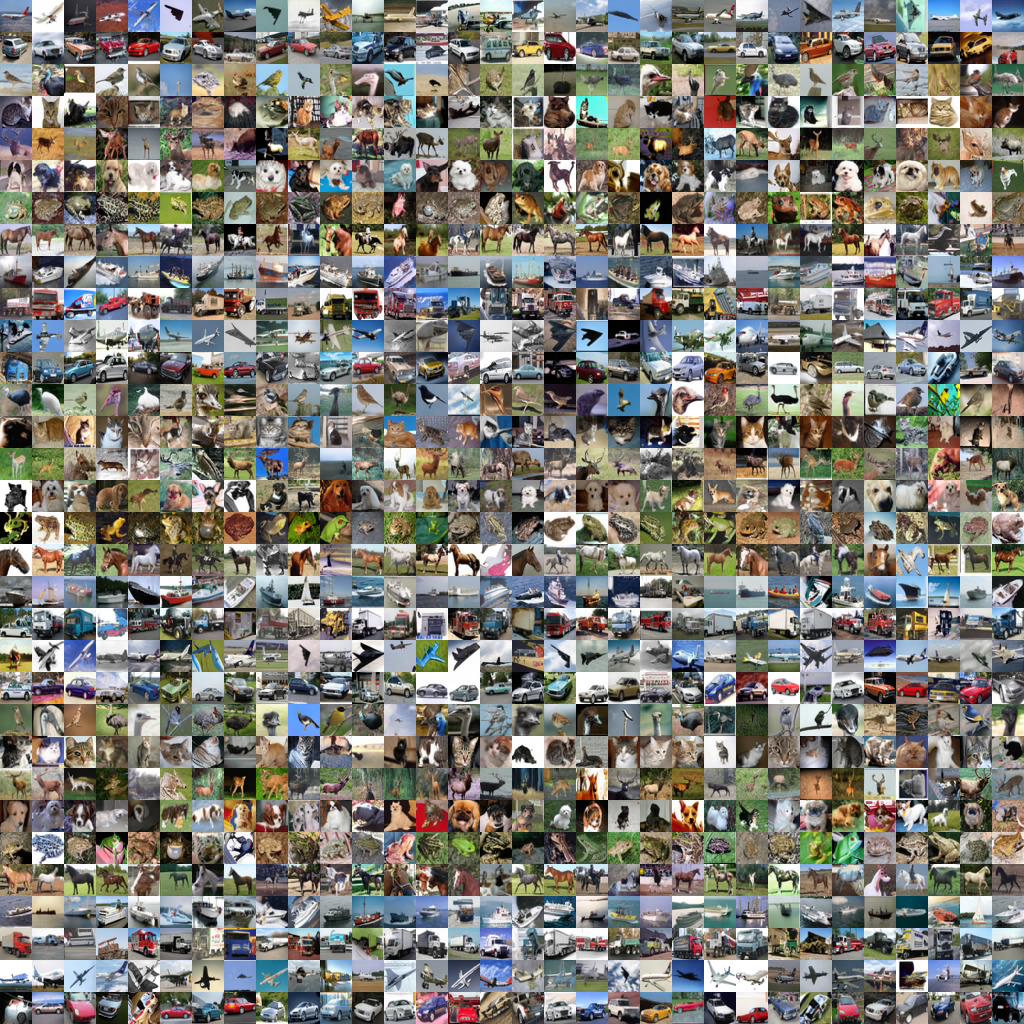
\includegraphics[width=\linewidth]{figures/qualitative/cifar-10-000222209.jpg}
    \caption{Qualitative examples of sample generation from our Config E on CIFAR-10.}
    \label{fig:cifar10}
\end{figure}
}
{
% Variable to control the size of each image
\begin{figure}[ht!]
    %\newlength{\imgsize}
    \setlength{\imgsize}{0.2\linewidth} % Adjust this value to change the size of the images
    
    \setlength{\tabcolsep}{0pt} % Remove spacing between columns
    \renewcommand{\arraystretch}{0} % Remove spacing between rows

    % New command to include images from a specific directory
    \newcommand{\qualitativeimg}[1]{%
        \includegraphics[width=\imgsize]{figures/qualitative/stacked-mnist-000008806/number-#1.jpg}%
    }
    \centering
    
    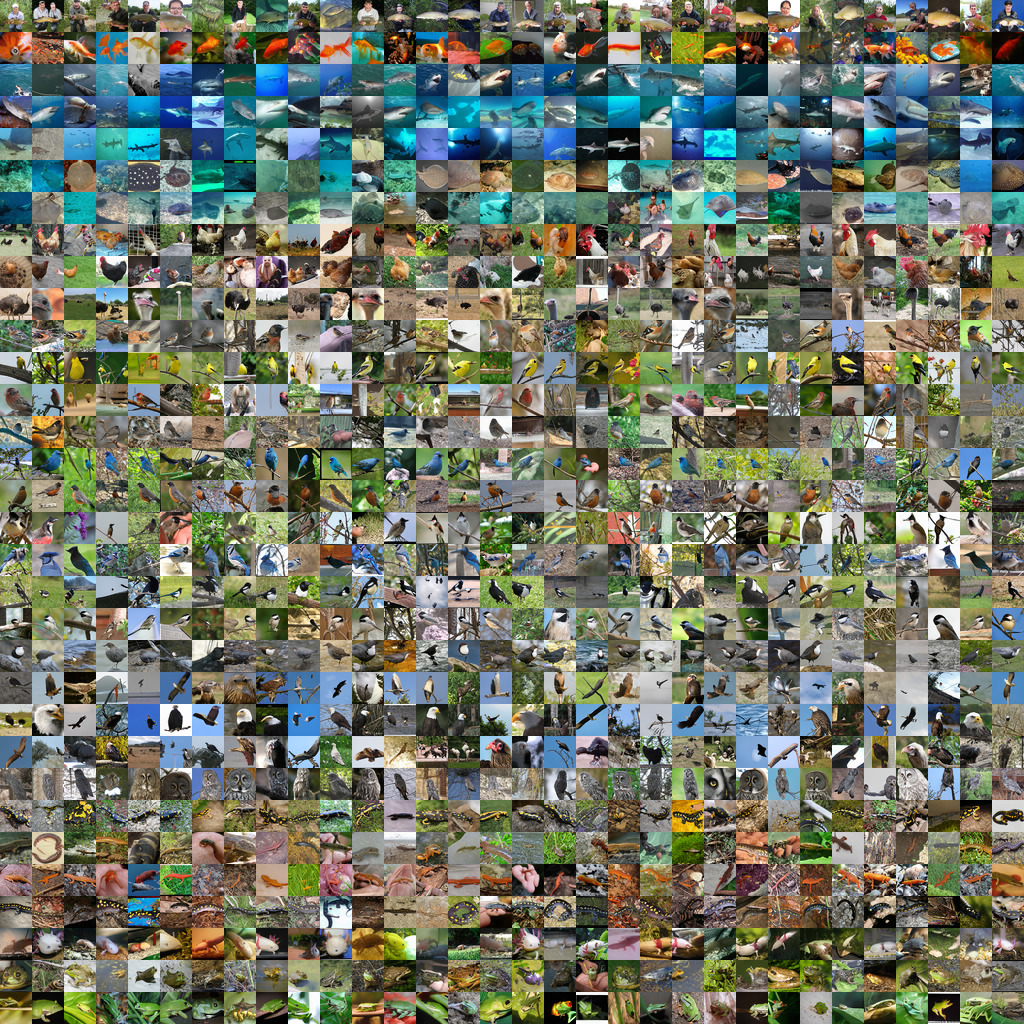
\includegraphics[width=\linewidth]{figures/qualitative/imgnet-32-000681275.jpg}
    \caption{Qualitative examples of sample generation from our Config E on ImageNet-32.}
    \label{fig:imgnet-32}
\end{figure}
}
%% \begin{figure}
%     \centering
%     \includegraphics{figures/FID-vs-Params-Plot.eps}
%     \caption{This scatter-plot shows the FID performance of our model on FFHQ-256 vs the number of parameters when only trained for 5million steps}
%     \label{fig:fid-vs-params-ablation}
% \end{figure}


\section{A Roadmap to a New Baseline --- \modelName}
\label{sec:roadmap}

% \vk{What about naming the new GAN that is being proposed? SimpleGAN...?}\jt{R3GAN...?}

% \vk{My main comment about this section is that it reads like mix of methods and experiments: all the experimental details/results (e.g., we set the learning rate to $10^{-4}$) should be under experiments (but you can still describe the key important takeaways here, e.g., we need a smaller learning rate)}

The well-behaved RpGAN + $R_1$ + $R_2$ loss alleviates GAN optimization problems, and lets us proceed to build a minimalist baseline---\modelName---with recent network backbone advances in mind~\cite{convnext,metaformer}. Rather than simply state the new approach, we will draw out a roadmap from the StyleGAN2 baseline~\cite{sg2ada}. This model (Config A; identical to~\cite{sg2ada}) consists of a VGG-like~\cite{vgg} backbone for $G$, a ResNet $D$, a few techniques that facilitate style-based generation, and many tricks that serve as patches to the weak backbone. Then, we remove all non-essential features of StyleGAN2 (Config B), apply our loss function (Config C), and gradually modernize the network backbone (Config D-E).


We evaluate each configuration on FFHQ $256\times256$~\cite{sg1}. Network capacity is kept roughly the same for all configurations---both $G$ and $D$ have about 25\ M trainable parameters. Each configuration is trained until $D$ sees 5\ M real images. We inherit training hyperparameters (\eg, optimizer settings, batch size, EMA decay length) from Config A unless otherwise specified. We tune the training hyperparameters for our final model and show the converged result in Sec.~\ref{sec:exp}.

%\paragraph{StyleGAN2 (Config A).}This configuration is identical to the baseline~\cite{sg2ada} with the style-based generator and all tricks enabled.  

\vspace{-0.3cm}
\paragraph{Minimum baseline (Config B).}
\begin{wraptable}[21]{r}{8cm}
\vspace{-0.5cm}
\resizebox{1\linewidth}{!}{
\begin{tabular}{ l r c c c } 
\toprule
   & \multicolumn{1}{l}{Configuration}  & FID$\downarrow$                    & G \#params              & D \#params               \\ 
\midrule
A  & \multicolumn{1}{l}{StyleGAN2}  & 7.516                  & 24.767M                  & 24.001M                   \\
\midrule
B  & \multicolumn{1}{l}{Stripped StyleGAN2}                                                                                                                                                                                                                                                                                                                                                                                                                 &                        &                          &                           \\ 
   & \begin{tabular}[c]{@{}r@{}}\textcolor{red}{- $z$ normalization}\\ \textcolor{red}{- Minibatch stddev}\\ \textcolor{red}{- Equalized learning rate}\textcolor{red}{}\\\textcolor{red}{- Mapping network}\\ \textcolor{red}{- Style injection}\\ \textcolor{red}{- Weight mod / demod}\\ \textcolor{red}{- Noise injection}\\ \textcolor{red}{- Mixing regularization}\\ \textcolor{red}{- Path length regularization}\\ \textcolor{red}{- Lazy regularization}\textcolor{blue}{}\end{tabular} & \multirow{2}{*}{12.46} & \multirow{2}{*}{18.890M} & \multirow{2}{*}{23.996M}  \\ 
\midrule
C  & \multicolumn{1}{l}{Well-behaved Loss}                       &                        &                          &                           \\ 
 & \textcolor[rgb]{0,0.502,0.502}{+ RpGAN loss}                                                                                                                                                                                                                                                                                                                                                                                                                   & 11.77                                           & \multirow{2}{*}{18.890M} & \multirow{2}{*}{23.996M}                           \\ 
   & \textcolor[rgb]{0,0.502,0.502}{+ $R_2$ gradient penalty}                                                                                                                                                                                                                                                                                                                                                                                                & \multirow{1}{*}{11.65} &                          &                           \\ 
\midrule
D  & \multicolumn{1}{l}{ConvNeXt-ify pt.~1}                                                                                                                                                                                                                                                                                                                                                                                                                 &                        &                          &                           \\ 
 & \textcolor[rgb]{0,0.502,0.502}{+ ResNet-ify G $\&$ D}                                                                                                                                                                                                                                                                                                                                                                                                   & 10.17                  & 23.400M                  & \multirow{2}{*}{23.282M}  \\
   & \textcolor{red}{- Output skips}                                                                                                                                                                                                                                                                                                                                                                                                                         & 9.950 & 23.378M &                           \\ 
\midrule
E  & \multicolumn{1}{l}{ConvNeXt-ify pt.~2}                              &                        &                          &                           \\
 & \textcolor[rgb]{0,0.502,0.502}{+ ResNeXt-ify G $\&$ D}                                                                                                                                                                                                                                                                                                                                                                                                  & 7.507                  & 23.188M                  & 23.091M                   \\ 
   & \textcolor[rgb]{0,0.502,0.502}{+ Inverted bottleneck}                                                                                                                                         & 7.045 & 23.058M & 23.010M  \\ 
\bottomrule
\end{tabular}
}
\vspace{-0.25cm}
\caption{Effect of our simplification and modernization efforts evaluted on FFHQ-256.} 
\label{tab:roadmap}
\end{wraptable}

%To find the essential elements that contribute to StyleGAN2's success, 
We strip away all StyleGAN2 features, retaining only the raw network backbone and basic image generation capability. The features fall into three categories:
\begin{itemize}[leftmargin=10pt,itemsep=0pt,topsep=0pt]
\item Style-based generation: mapping network~\cite{sg1}, style injection~\cite{sg1}, weight modulation/demodulation~\cite{sg2}, noise injection~\cite{sg1}.
\end{itemize}\quad % JT: Weird but intential LaTeX
\begin{itemize}[leftmargin=10pt,itemsep=0pt,topsep=0pt]
\vspace{-0.25cm} % JT: Weird but intentional LaTeX
\item Image manipulation enhancements: mixing regularization~\cite{sg1}, path length regularization~\cite{sg2}.
\item Tricks: $z$ normalization~\cite{pggan}, minibatch stddev~\cite{pggan}, equalized learning rate~\cite{pggan}, lazy regularization~\cite{sg2}.
\end{itemize}

% Such features could be reintroduced as per application need (e.g., style injection). 
Following~\cite{sgxl,sg-t}, we reduce the dimension of $z$ to 64. The absence of equalized learning rate necessitates a lower learning rate, reduced from 2.5$\times$10\textsuperscript{-3} to 5$\times$10\textsuperscript{-5}. Despite a higher FID of 12.46 than Config-A, this simplified baseline produces reasonable sample quality and stable training. We compare this with DCGAN~\cite{dcgan}, an early attempt at image generation. Key differences include:
\begin{enumerate}[label=\alph*), noitemsep,topsep=0pt,leftmargin=24pt]
\item Convergent training objective with $R_1$ regularization.\label{item:convergent} 
\item Smaller learning rate, avoiding momentum optimizer (Adam $\beta_1=0$).\label{item:learning_rate} 
\item No normalization layer in $G$ or $D$.\label{item:normalization} 
\item Proper resampling via bilinear interpolation instead of strided (transposed) convolution.\label{item:resampling} 
\item Leaky ReLU in both $G$ and $D$, no tanh in the output layer of $G$.\label{item:activation} 
\item 4$\times$4 constant input for $G$, output skips for $G$, ResNet $D$.\label{item:input} 
\end{enumerate}

\textbf{Experimental findings from StyleGAN.} Violating \ref{item:convergent}, \ref{item:learning_rate}, or \ref{item:normalization} often leads to training failures.
%, contributing to the reputation that GANs as difficult to train. 
Gidel~\etal~\cite{ganmomentum} show that \emph{negative} momentum can improve GAN training dynamics. Since optimal negative momentum is another challenging hyperparameter, we do not use any momentum to avoid worsening GAN training dynamics. Studies suggest normalization layers harm generative models~\cite{sg2,edm2}. Batch normalization~\cite{bn} often cripples training due to dependencies across multiple samples, and is incompatible with $R_1$, $R_2$, or RpGAN that assume independent handling of each sample. Weaker data-independent normalizations~\cite{sg2,edm2} might help; we leave this for future work. Early GANs may succeed despite violating \ref{item:convergent} and \ref{item:normalization}, possibly constituting a full-rank solution~\cite{r1} to Eq.~\ref{eq:gan}.

Violations of \ref{item:resampling} or \ref{item:activation} do not significantly impair training stability but negatively affect sample quality. Improper transposed convolution can cause checkerboard artifacts, unresolved even with subpixel convolution~\cite{subpixel} or carefully tuned transposed convolution unless a low-pass filter is applied. Interpolation methods avoid this issue, varying from nearest neighbor~\cite{pggan} to Kaiser filters~\cite{sg3}. We use bilinear interpolation for simplicity. For activation functions, smooth approximations of (leaky) ReLU, such as Swish~\cite{swish}, GELU~\cite{gelu}, and SMU~\cite{smu}, worsen FID. PReLU~\cite{prelu} marginally improves FID but increases VRAM usage, so we use leaky ReLU.

All subsequent configurations adhere to \ref{item:convergent} through \ref{item:activation}. Violation of \ref{item:input} is acceptable as it pertains to the network backbone of StyleGAN2~\cite{sg2}, modernized in Config D and E.

% \paragraph{Minimum baseline (Config B).}
% To elucidate the implementation details that contribute to the success of StyleGAN2, we remove all the StyleGAN2 features until only the raw network backbone and basic image generation capability are retained. The list of removed features can be placed into three categories:
% \begin{itemize}
%     \item Style-based generation: mapping network~\cite{sg1}, style injection~\cite{sg1}, weight modulation / demodulation~\cite{sg2}, noise injection~\cite{sg1}.
%     \item Image manipulation enhancements: mixing regularization~\cite{sg1}, path length regularization~\cite{sg2}.
%     \item Tricks: $z$ normalization~\cite{pggan}, minibatch stddev~\cite{pggan}, equalized learning rate~\cite{pggan}, lazy regularization~\cite{sg2}.
% \end{itemize}
% The first two categories are technically orthogonal to our work; we remove them along with the tricks as our goal is to build a minimalist baseline and they can be reintroduced to our model in the future. \aaron{For this work, we want to keep our baseline as simple as possible, and demonstrate that many of these additions are not necessary for training a state of the art GAN. Instead, we ask what the simplest architecture one can design that can be used to train a GAN.}\vk{Do you include back the things you remove? Curious why / why not} Following~\cite{sgxl,sg-t}, we decrease the dimension of $z$ to 64. The removal of equalized learning rate necessitates a significantly lower learning rate and we decrease the learning rate from $2.5\times10^{-3}$ to $5\times10^{-5}$, any higher learning rate cripples training. This highly simplified baseline, despite achieving a considerably worse FID of 12.46, produces quite reasonable sample quality and training is stable. We compare this baseline against DCGAN~\cite{dcgan}, a barely working early GAN attempt at image generation. Notable differences include:
% \begin{enumerate}[label=\alph*)]
%     \item Convergent training objective with $R_1$ regularization.
%     \item Smaller learning rate, not using a momentum optimizer (Adam $\beta_1=0$).
%     \item Neither $G$ nor $D$ uses any normalization layer.
%     \item Proper resampling via bilinear interpolation instead of strided (transposed) convolution.
%     \item Leaky ReLU in both $G$ and $D$, no tanh in the output layer of $G$.
%     \item $4\times4$ constant input for $G$, output skips for $G$, ResNet $D$.
% \end{enumerate}

% \vk{Part B too verbose and many of these details can be in appendix  or removed }
% Our experiments show that any violation of a), b), or c) can easily lead to training failures, and these violations likely earned GANs the reputation of being hard to train. Gidel~\etal~\cite{ganmomentum} show that momentum not only should be avoided for GAN optimization, but \emph{negative} momentum might even improve GAN training dynamics. Since the optimal negative momentum is another hard to tune hyperparameter, we simply do not use any momentum to at least not worsen the GAN training dynamics. Recent studies~\cite{sg2,edm2} on GANs and diffusion models show that normalization layers harm generative models. Batch normalization~\cite{bn} in particular often cripples training as it establishes dependency across multiple samples and it is therefore incompatible with $R_1$, $R_2$ or RpGAN, all of which assume that the networks handle each sample independently. Although weaker data-independent normalizations~\cite{sg2,edm2} might still help, we leave these as future work and do not employ any normalization technique. A curious case with many early GANs is that the simultaneous violation of a) and c) (\eg using batch normalization and not using any gradient penalty) occasionally leads to successful training. One possible explanation is that this might constitute a full-rank solution~\cite{r1} to Eq.\ref{eq:gan} which is also locally convergent.

% Violations of d) or e) do not impair training stability much, however, these violations are detrimental to sample quality. Upsampling with improper transposed convolution can result in imbalanced overlaps between pixels which lead to checkerboard artifacts. The artifacts cannot be fully resolved even when the imbalanced overlap problem is eliminated by subpixel convolution~\cite{subpixel} or carefully tuned transposed convolution unless a proper low-pass filter is applied. Interpolation in comparison avoids such failure directly from the source. The choice of the interpolation method varies wildly in previous works, from naive approaches such as nearest neighbor~\cite{pggan} to advanced resampling techniques such as Kaiser filters~\cite{sg3}, we retain the choice of bilinear interpolation for simplicity. For the activation function, we experiment with various smooth approximations of (leaky) ReLU including Swish~\cite{swish}, GELU~\cite{gelu} and SMU~\cite{smu}, all of which deteriorate FID considerably. The only activation function we find to marginally improve FID is PReLU~\cite{prelu}, however, the tiny improvement does not justify the considerably higher VRAM usage, and therefore we settle for leaky ReLU.

% For all subsequent configurations, we ensure compliance to a) through e). We are free to violate f) as this is merely the network backbone adopted by StyleGAN2~\cite{sg2} and we modernize the backbone in Config D and E.

\vspace{-0.3cm}
\paragraph{Well-behaved loss function (Config C).}
% Given the simplified baseline, we move on to the modernization part of the roadmap. We first modernize the loss function so that the representation power of modern network backbones will not be compromised by GAN optimization difficulties. 
We use the loss function proposed in Section~\ref{sec:loss} and this reduces FID to 11.65. We hypothesize that the network backbone in Config B is the limiting factor. 
% and expect more drastic improvements as further modernization takes place.


\begin{figure*}[t]%
\centering\footnotesize%
 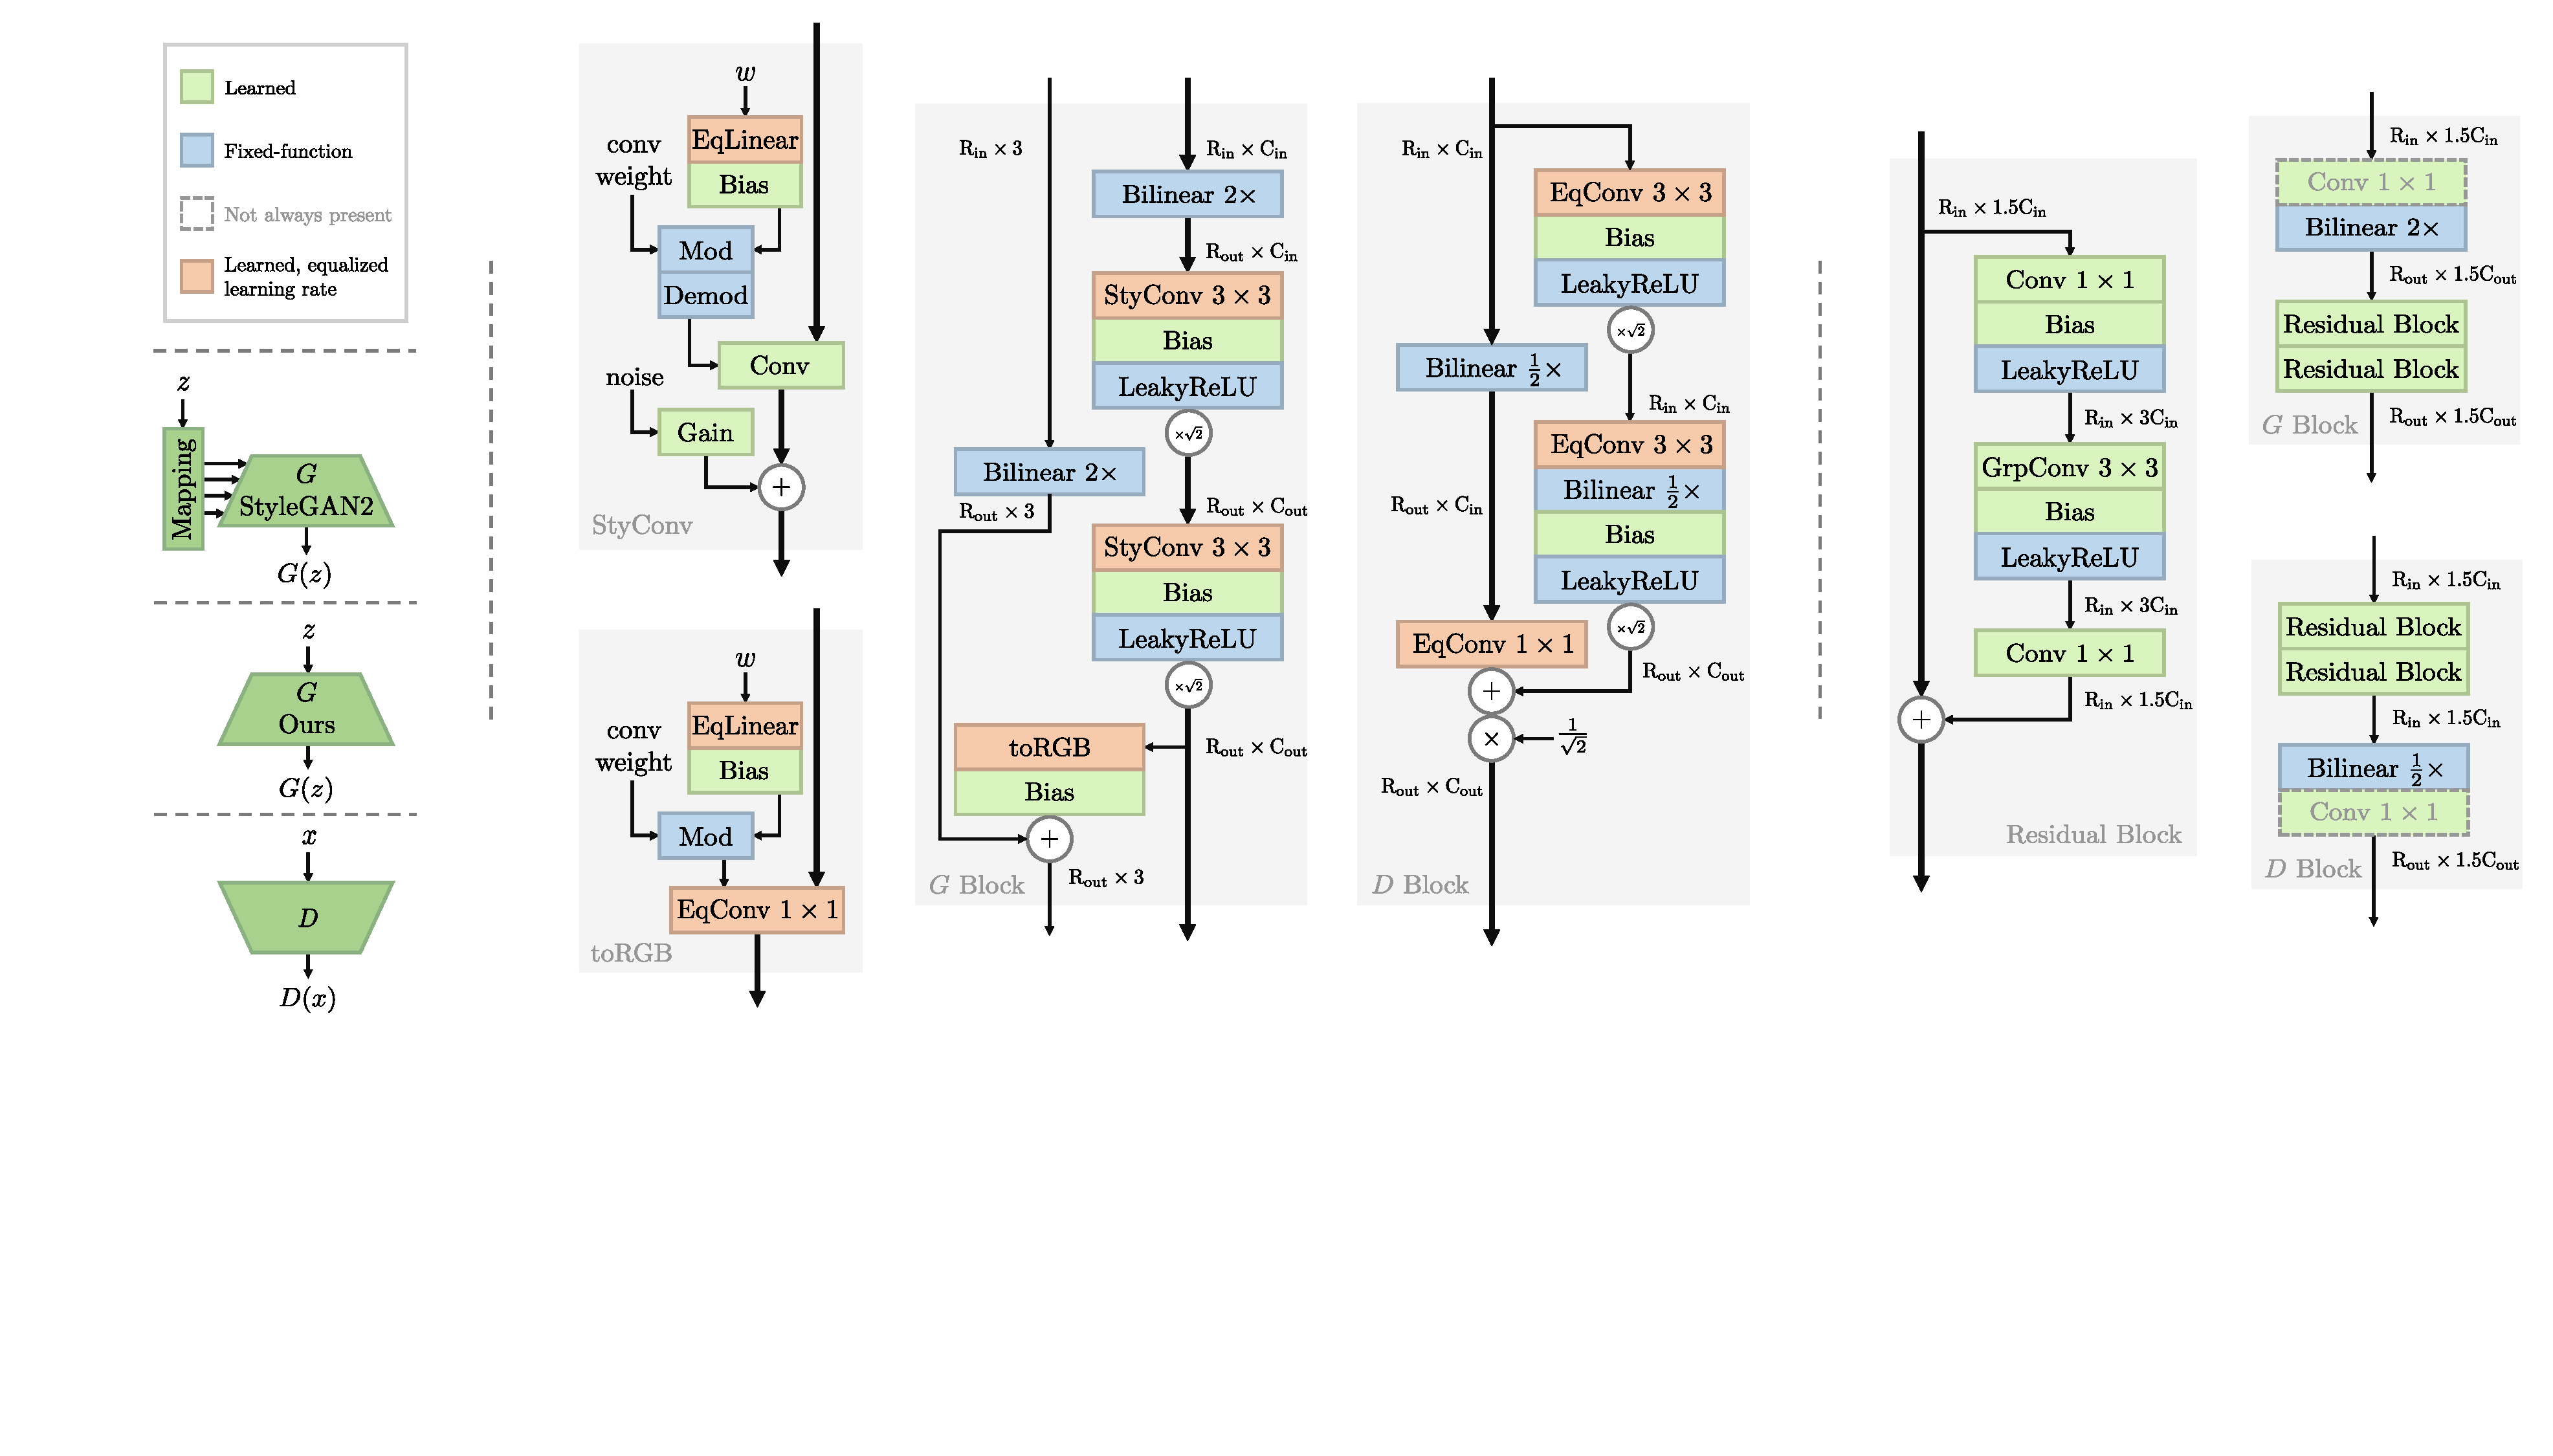
\includegraphics[width=\linewidth,clip,trim={3.5cm 11.5cm 0cm 0cm}]{figures/arch.pdf}\\%
\makebox[0.144\linewidth]{(a) Overall view}\hfill%
\makebox[0.562\linewidth]{(b) StyleGAN2 architecture blocks~\cite{sg2} (Config A)}\hfill%
\makebox[0.294\linewidth]{(c) Ours (Config E)}\hfill%
\vspace{0.5mm}
\caption{\label{fig:network}%
\textbf{Architecture comparison.}
For image generation, $G$ and $D$ are often both deep ConvNets with either partially or fully symmetric architectures.
\textbf{(a)}
StyleGAN2~\cite{sg2} $G$ uses a network to map noise vector $z$ to an intermediate style space $\mathcal{W}$. We use a traditional generator as style mapping is not necessary for a minimal working model.
\textbf{(b)}
StyleGAN2's building blocks have intricate layers but are themselves simple, with a ConvNet architecture from 2015~\cite{alexnet,vgg,resnet}. ResNet's identity mapping principle is also violated in the discriminator.
\textbf{(c)}
We remove tricks and modernize the architecture. Our design has clean layers with a more powerful ConvNet architecture.
}%
\vspace{-0.3cm}%
\end{figure*}

\vspace{-0.3cm}
\paragraph{General network modernization (Config D).}
First, we apply the 1-3-1 bottleneck ResNet architecture~\cite{resnet,resnet2} to both $G$ and $D$. This is the direct ancestor of all modern vision backbones~\cite{convnext,metaformer}. 
% However, rather than precisely replicating the architecture in~\cite{resnet2}, 
We also incorporate principles discovered in Config B and various modernization efforts from ConvNeXt~\cite{convnext}. We categorize the roadmap of ConvNeXt as follows:
% \begin{enumerate}[label=\roman*)]
%     \item Consistently beneficial: 1) increased width with depthwise conv. 2) inverted bottleneck. 3) fewer activation functions. 4) separate resampling layers.
%     \item Negligible performance gain: 1) large kernel depthwise conv with fewer channels. 2) replacing ReLU with GELU. 3) fewer normalization layers. 4) replacing batch norm with layer norm.
%     \item Irrelevant to our problem setting: 1) improved training recipe. 2) stage ratio. 3) "patchify" stem.
% \end{enumerate}
% % We are interested in applying i) to our model, among which i.3) and i.4) are applicable to the classic ResNet. We leave i.1) and i.2) for Config E. Much of ii) were introduced merely for the sake of mimicking vision transformers~\cite{swin,vit} even though they fail to bring any significant improvement~\cite{convnext}. ii.3) and ii.4) are inapplicable since we do not use any normalization layer following principle c). ii.2) is directly at odds with our finding that GELU deteriorates GAN performance, and we use leaky ReLU as in principle e). Liu~\etal put heavy emphasis on using large conv kernels (ii.1)~\cite{convnext}, however this results in slightly but consistently worse performance than using wider $3\times3$ conv layers and we therefore do not employ this design choice of ConvNeXt.

% We aim to apply i) to our model, specifically i.3) and i.4) for the classic ResNet, while reserving i.1) and i.2) for Config E. Many aspects of ii) were introduced merely to mimic vision transformers~\cite{swin,vit} without yielding significant improvements~\cite{convnext}. ii.3) and ii.4) are inapplicable due to our avoidance of normalization layers following principle c). ii.2) contradicts our finding that GELU deteriorates GAN performance, thus we use leaky ReLU per principle e). Liu~\etal emphasize large conv kernels (ii.1)~\cite{convnext}, but this results in slightly worse performance compared to wider $3\times3$ conv layers, so we do not adopt this ConvNeXt design choice.
%
\begin{enumerate}[label=\roman*., itemsep=1pt,leftmargin=12pt,topsep=0pt,parsep=1pt]
    \item Consistently beneficial: \begin{enumerate*}[label=\theenumi\arabic*), ref=\arabic*, before=\unskip{ }, itemjoin={{, }}, itemjoin*={{, and }}]
        \item\label{item:i1} increased width with depthwise convolution
        \item\label{item:i2} inverted bottleneck
        \item\label{item:i3} fewer activation functions
        \item\label{item:i4} separate resampling layers.
    \end{enumerate*}
    \item Negligible performance gain: \begin{enumerate*}[label=\theenumi\arabic*), ref=\arabic*, before=\unskip{ }, itemjoin={{, }}, itemjoin*={{, and }}]
        \item\label{item:ii1} large kernel depthwise conv.~with fewer channels
        \item\label{item:ii2} swap ReLU with GELU
        \item\label{item:ii3} fewer normalization layers
        \item\label{item:ii4} swap batch norm.~with layer norm.
    \end{enumerate*}
    \item Irrelevant to our setting: \begin{enumerate*}[label=\theenumi\arabic*), ref=\arabic*, before=\unskip{ }, itemjoin={{, }}, itemjoin*={{, and }}]
        \item\label{item:iii1} \hspace{-0.1cm}improved training recipe
        \item\label{item:iii2} \hspace{-0.1cm}stage ratio
        \item\label{item:iii3} \hspace{-0.1cm}`patchify' stem.
    \end{enumerate*}
\end{enumerate}

We aim to apply i) to our model, specifically i.\ref{item:i3} and i.\ref{item:i4} for the classic ResNet, while reserving i.\ref{item:i1} and i.\ref{item:i2} for Config E. Many aspects of ii) were introduced merely to mimic vision transformers~\cite{swin,vit} without yielding significant improvements~\cite{convnext}. ii.\ref{item:ii3} and ii.\ref{item:ii4} are inapplicable due to our avoidance of normalization layers following principle \ref{item:normalization}. ii.\ref{item:ii2} contradicts our finding that GELU deteriorates GAN performance, thus we use leaky ReLU per principle \ref{item:activation}. Liu~\etal emphasize large conv.~kernels (ii.\ref{item:ii1})~\cite{convnext}, but this results in slightly worse performance compared to wider 3$\times$3 conv.~layers, so we do not adopt this ConvNeXt design choice.

\paragraph{Neural network architecture details.} Given i.\ref{item:i3}, i.\ref{item:i4}, and principles \ref{item:normalization}, \ref{item:resampling}, and \ref{item:activation}, we can replace the StyleGAN2 backbone with a modernized ResNet. We use a fully symmetric design for $G$ and $D$ with 25\ M parameters each, comparable to Config-A. The architecture is minimalist: each resolution stage has one transition layer and two residual blocks. The transition layer consists of bilinear resampling and an optional 1$\times$1 conv.~for changing spatial size and feature map channels. The residual block includes five operations: Conv1$\times$1$\rightarrow$ Leaky ReLU $\rightarrow$ Conv3$\times$3$\rightarrow$ Leaky ReLU $\rightarrow$ Conv1$\times$1, with the final Conv1$\times$1 having no bias term. For the 4$\times$4 resolution stage, the transition layer is replaced by a basis layer for $G$ and a classifier head for $D$. The basis layer, similar to StyleGAN~\cite{sg1,sg2}, uses 4$\times$4 learnable feature maps modulated by $z$ via a linear layer. The classifier head uses a global 4$\times$4 depthwise conv.~to remove spatial extent, followed by a linear layer to produce $D$'s output. We maintain the width ratio for each resolution stage as in Config A, making the stem width 3$\times$ as wide due to the efficient 1$\times$1 conv. The 3$\times$3 conv.~in the residual block has a compression ratio of 4, following~\cite{resnet,resnet2}, making the bottleneck width 0.75$\times$ as wide as Config A.
%Given i.3), i.4) and principles c), d), and e), we are now ready to replace the StyleGAN2 backbone with a modernized ResNet. We adopt a fully symmetric design for $G$ and $D$, and make the model size comparable to Config A, both $G$ and $D$ have approximately 25M parameters. We keep the architecture as minimalist as possible, for each resolution stage, we have one transition layer and two residual blocks. The transition layer consists of bilinear resampling and an optional $1\times1$ conv that allows us to change the spatial size and the number of channels of the feature maps. The residual block contains five consecutive operations on the residual branch: Conv$1\times1\rightarrow$ Leaky ReLU $\rightarrow$ Conv$3\times3\rightarrow$ Leaky ReLU $\rightarrow$ Conv$1\times1$, and the final Conv$1\times1$ has no bias term. For the $4\times4$ resolution stage, the transition layer is replaced by a basis layer for $G$ and a classifier head for $D$. The basis layer resembles the const input of StyleGAN~\cite{sg1,sg2} where a set of $4\times4$ learnable feature maps are modulated by $z$ via a linear layer. The classifier head first removes the spatial extent of the feature maps with a global $4\times4$ depthwise conv; the features are then fed to a linear layer to produce the output of $D$. We keep the width ratio for each resolution stage the same as Config A, and we are able to make the stem width $3\times$ as wide as Config A given the same model size thanks to the more efficient $1\times1$ conv. The compression ratio for the $3\times3$ conv in the residual block is set to 4 following~\cite{resnet,resnet2}, this makes the bottleneck width $0.75\times$ as wide as Config A.

% The lack of normalization necessitates more careful initialization for ResNet to avoid variance explosion. We apply fix-up initialization~\cite{fixup} to our modernized networks to remedy this. Concretely, we zero-initialize the last conv layer in each residual block, and scale down the initialization of the other two conv layers in the residual block by $L^{-0.25}$ where $L$ is the number of residual blocks in the network. We do not employ any other trick from fixup~\cite{fixup} such as applying excessive bias terms and the use of a scalar multiplier. The new network architecture and the initialization scheme allow us to raise the learning rate to $1\times10^{-4}$ without encountering training instability.
To avoid variance explosion due to the lack of normalization, we employ fix-up initialization~\cite{fixup}: 
%for our modernized networks: 
We zero-initialize the last convolutional layer in each residual block and scale down the initialization of the other two convolutional layers in the block by $L^{-0.25}$, where $L$ is the number of residual blocks. We avoid other fix-up tricks, such as excessive bias terms and a learnable multiplier.

% We show that removing all these architectural modifications of the original StyleGAN mildly harms performance, but not as much as one might expect in~\ref{sub:arc-experiments}. Furthermore, removing some components actually benefits FID.


% \begin{figure}
%     \centering
%     \includegraphics[width=0.25\linewidth]{example-image-a}

%     \caption{Swirl Figure. We show our model matches performance on Gaussian toy example. \aaron{Are we still doing a toy example}]}
%     \label{fig:enter-label}
% \end{figure}

% \begin{figure}
%     \centering
%     \includegraphics[width=0.25\linewidth]{example-image-b}
%     \caption{k-NN decision barrier. Intuitive example}
%     \label{fig:enter-label}
% \end{figure}

% \begin{figure*}
%     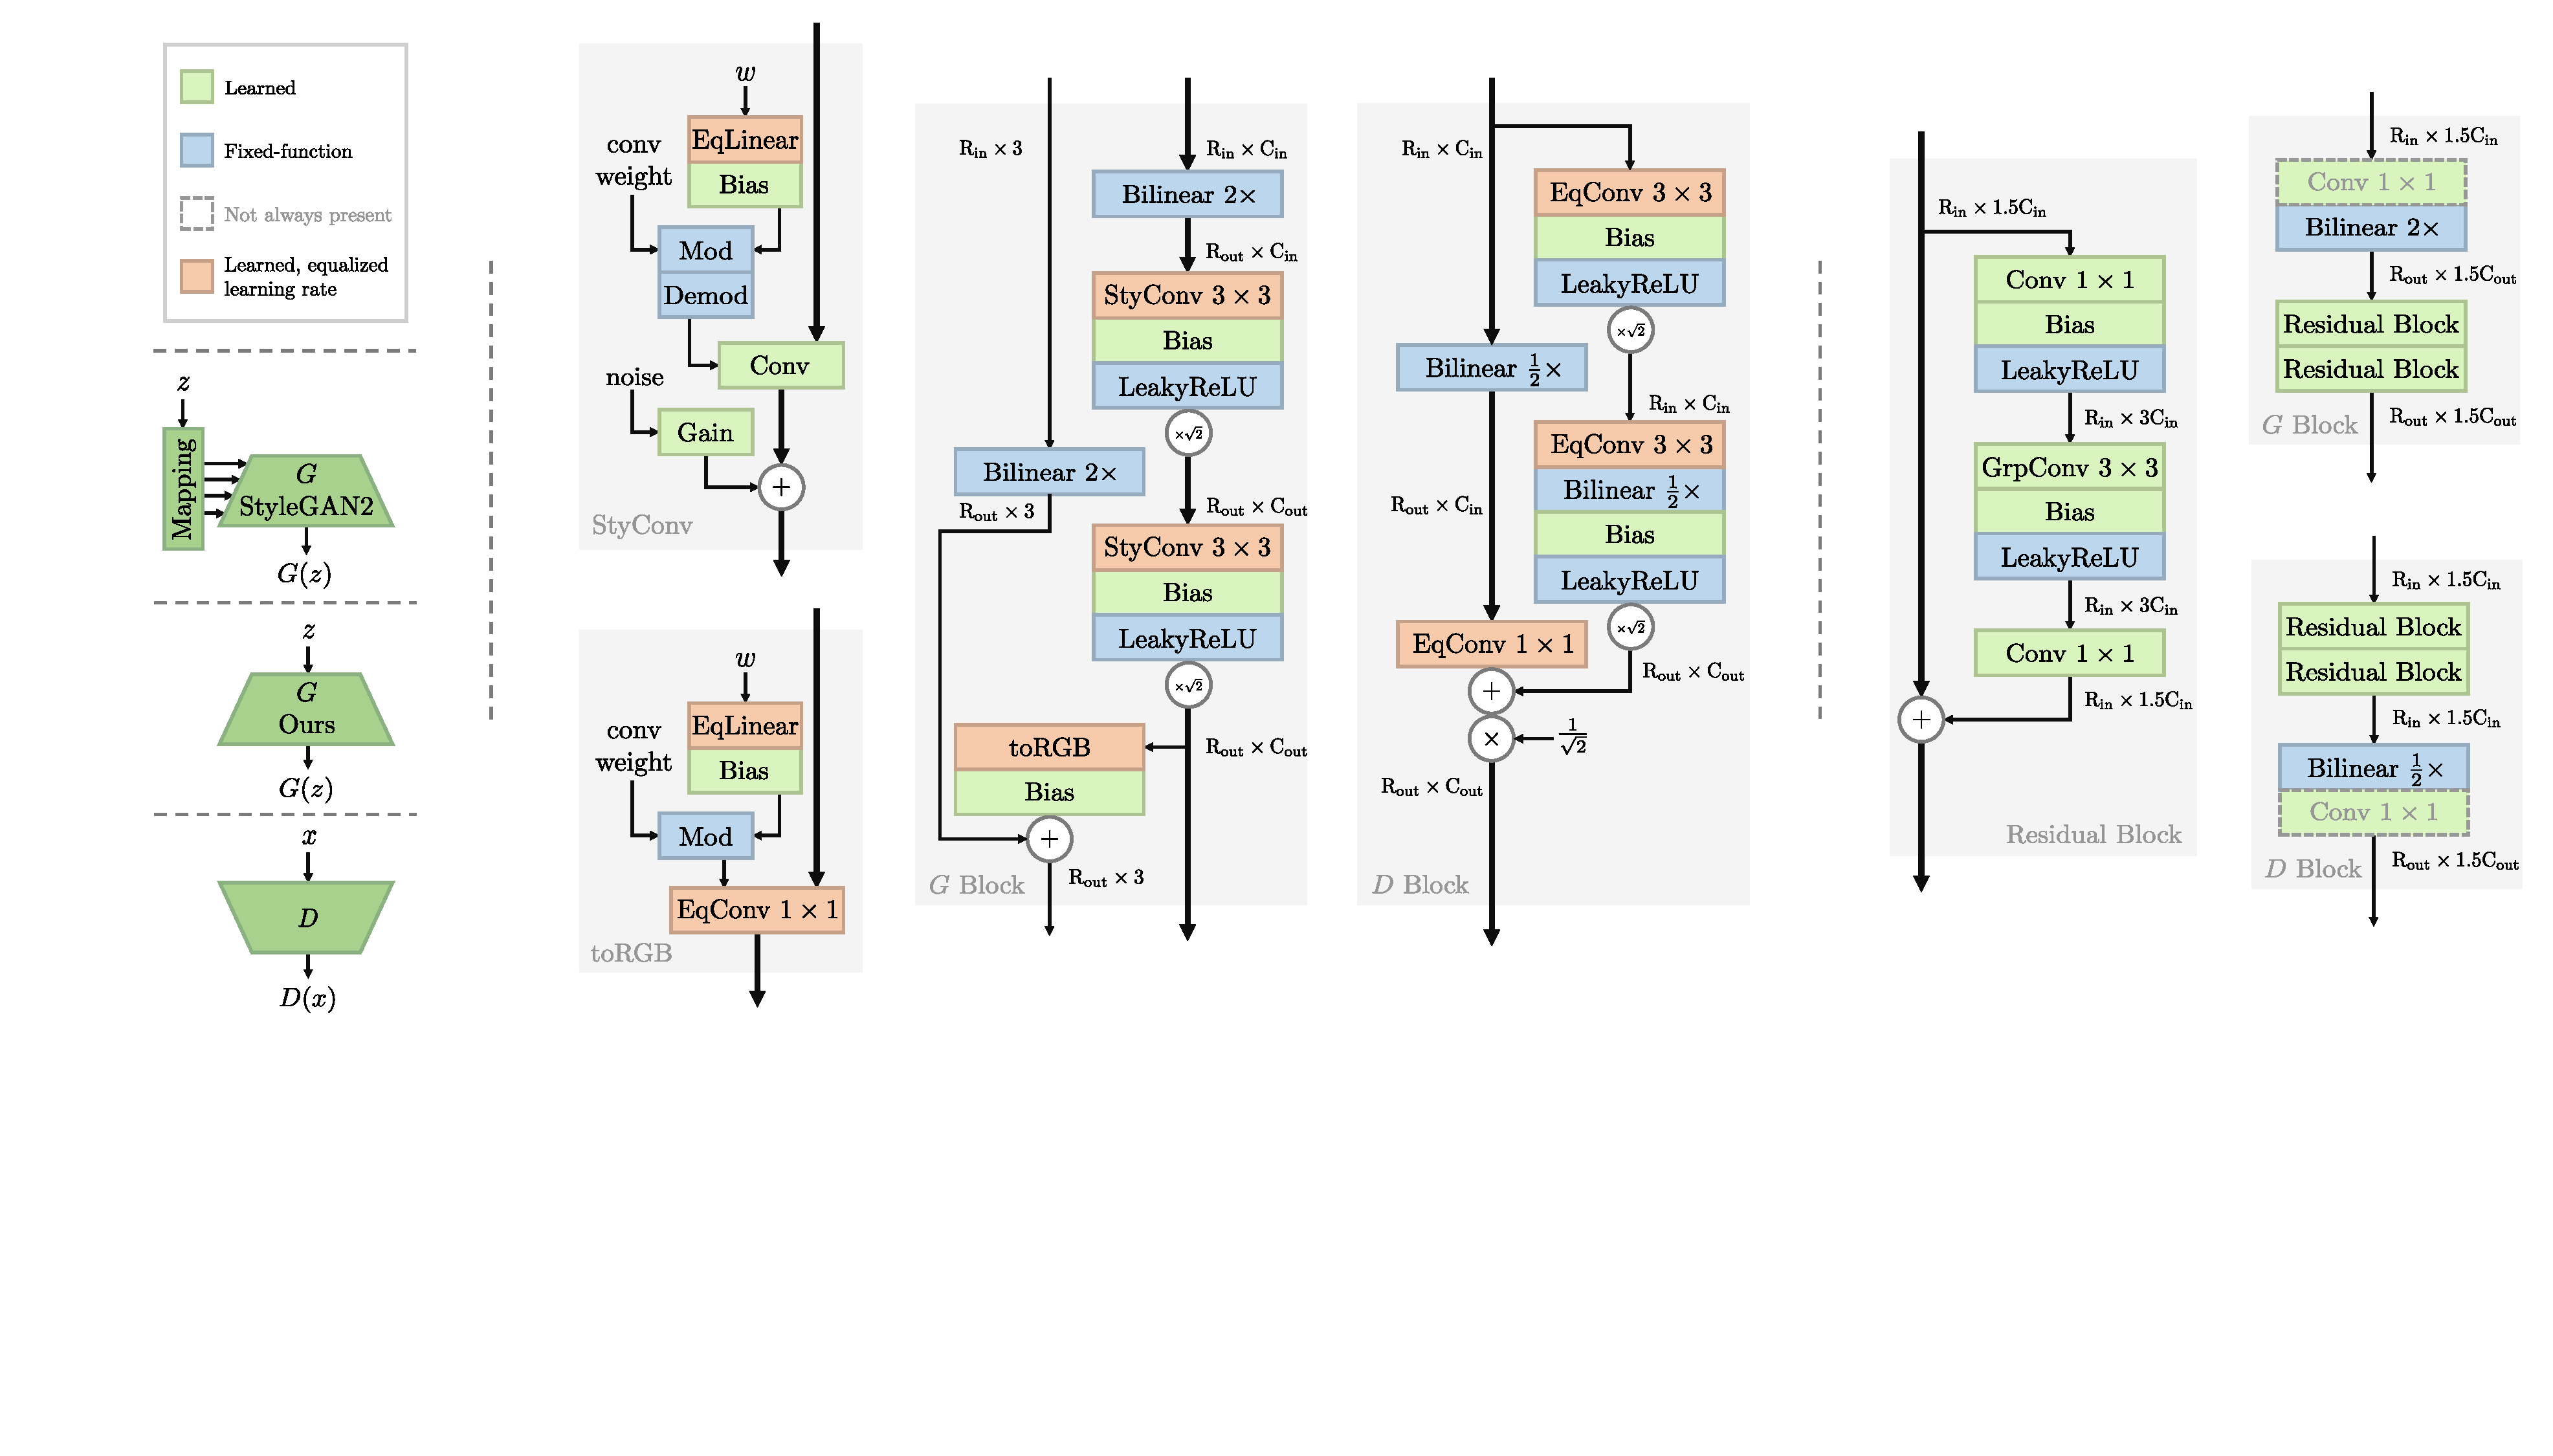
\includegraphics[width=\linewidth,clip,trim={3.5cm 11.5cm 0cm 0cm}]{figures/arch.pdf}
%     \vspace{-0.5cm}
%     \caption{\textbf{Network architecture block comparison to StyleGANv2}. \emph{Left:} High-level architectures. \emph{Middle:} StyleGANv2. \emph{Right:} Our simpler approach. Figure inspired by EDM2~\cite{edm2}.}
%     \label{fig:network}
% \end{figure*}





% \begin{wrapfigure}[16]{r}{8cm}
%     \vspace{-0.5cm}
%     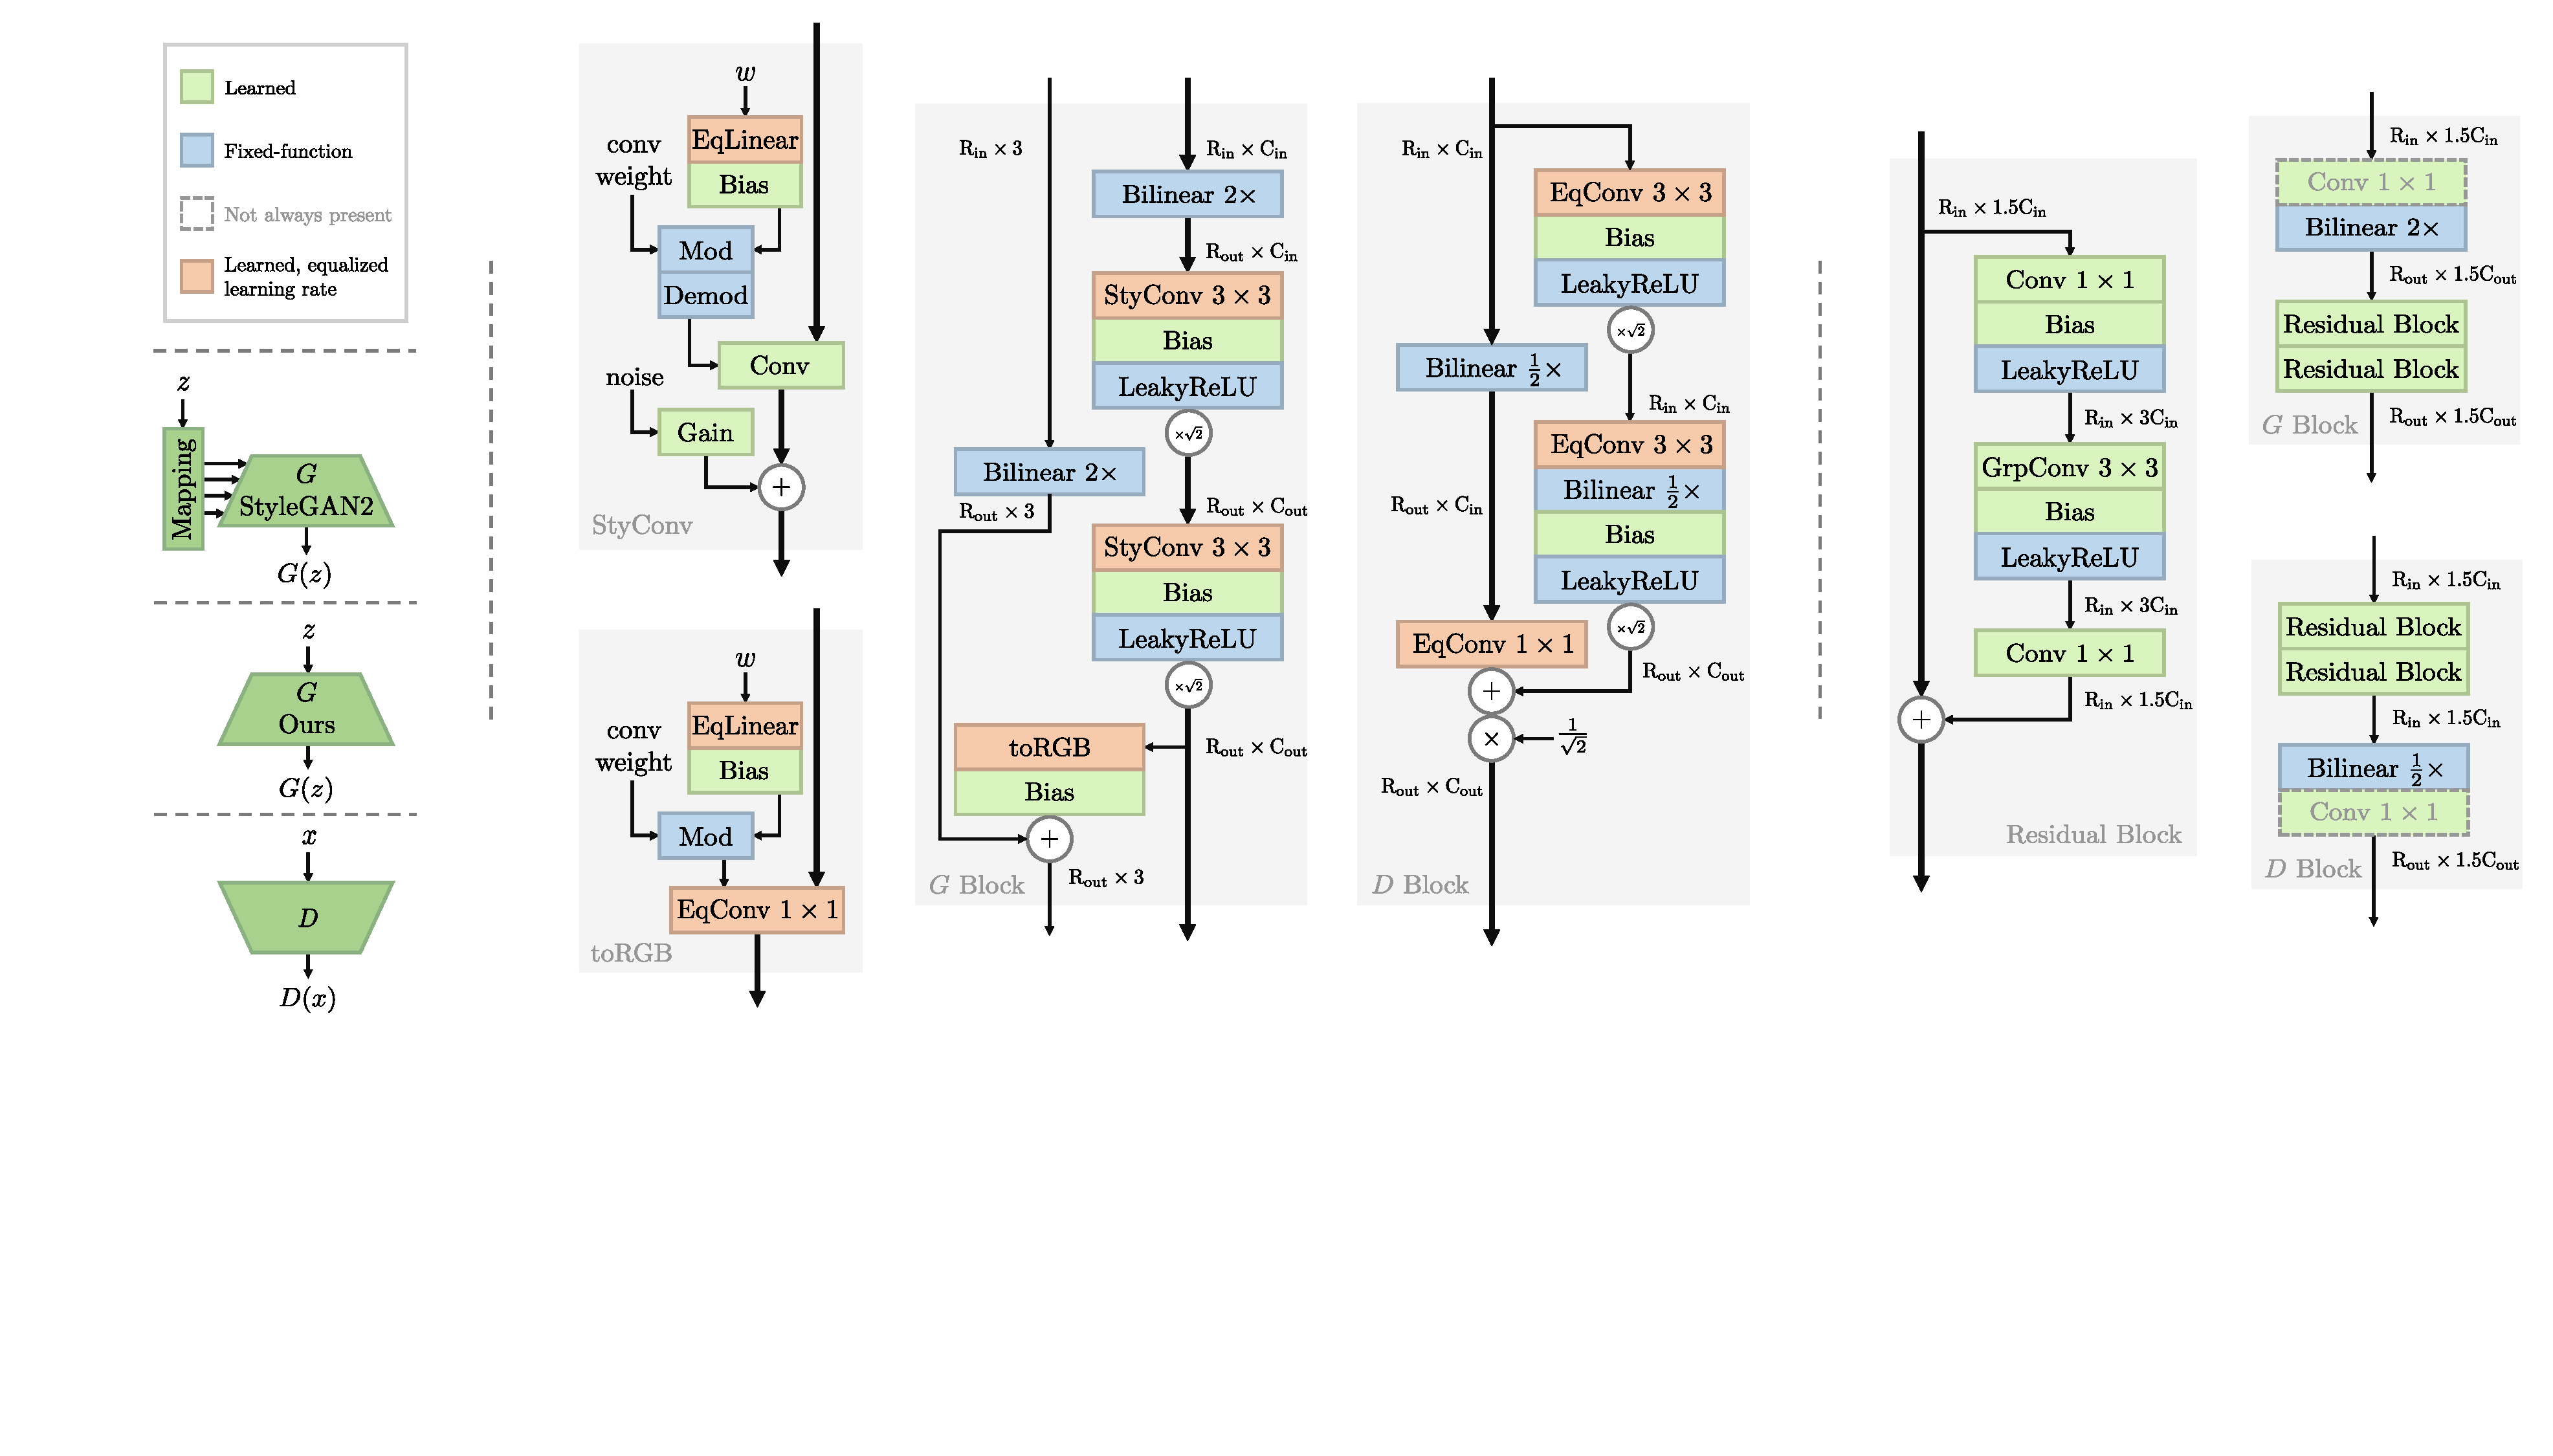
\includegraphics[width=1\linewidth,clip,trim={0cm 0cm 0cm 0cm}]{figures/arch.pdf}
%     \caption{Network architecture blocks.}
%     \label{fig:network}
% \end{wrapfigure}

\paragraph{Bottleneck modernization (Config E).}
Now that we have settled on the overall architecture, we investigate how the residual block can be modernized, specifically i.\ref{item:i1}) and i.\ref{item:i2}). First, we explore i.\ref{item:i1} and replace the 3$\times$3 convolution in the residual block with a grouped convolution. We set the group size to 16 rather than 1 (\ie depthwise convolution as in ConvNeXt) as depthwise convolution is highly inefficient on GPUs and is not much faster than using a larger group size. With grouped convolution, we can reduce the bottleneck compression ratio to two given the same model size. This increases the width of the bottleneck to 1.5$\times$ as wide as Config A. 
%With this, the FID drops to 7.51, surpassing the performance of StyleGAN2. 
Finally, we notice that the compute cost of grouped convolution is negligible compared to 1$\times$1 convolution, and so we seek to enhance the capacity of grouped convolution. We apply i.\ref{item:i2}), which inverts the bottleneck width and the stem width, and which doubles the width of grouped convolutions without any increase in model size. Figure~\ref{fig:network} depicts our final design, which reflects modern CNN architectures.
%\section{Discussion}
\label{sec:discussion}

We discuss related work, limitations, and some future directions.

\paragraph{Related Work.}
\cref{sec:discussion:selection} discusses how the selection mechanism relates to similar concepts.
\cref{sec:related} has an extended related work of SSMs and other related models.

\paragraph{No Free Lunch: Continuous-Discrete Spectrum.}
Structured SSMs were originally defined as discretizations of continuous systems \eqref{eq:ssm},
and have had a strong inductive bias toward continuous-time data modalities such as perceptual signals (e.g.\ audio, video).
As discussed in \cref{sec:method:motivation,sec:method:properties}, the selection mechanism overcomes their weaknesses
on discrete modalities such as text and DNA;
but this conversely can impede their performance on data that LTI SSMs excel on.
Our ablations on audio waveforms examine this tradeoff in more detail.

\paragraph{Downstream Affordances.}
Transformer-based foundation models (particularly LLMs) have a rich ecosystem of properties and modes of interaction with pretrained models,
such as fine-tuning, adaptation, prompting, in-context learning, instruction tuning, RLHF, quantization, and so on.
We are particularly interested in whether Transformer alternatives such as SSMs have similar properties and affordances.

%

\paragraph{Scaling.}
Our empirical evaluation is limited to small model sizes,
below the threshold of most strong open source LLMs (e.g. Llama \citep{touvron2023llama})
as well as other recurrent models such as RWKV~\citep{peng2023rwkv} and RetNet~\citep{sun2023retentive},
which have been evaluated at the 7B parameter scale and beyond.
It remains to assess whether Mamba still compares favorably at these larger sizes.
We also note that scaling SSMs may involve further engineering challenges and adjustments to the model
that are not discussed in this paper.

%


% \begin{figure}[14]{r}{8cm}
%     %\vspace{-0.25cm}
%     \centering
%     \includegraphics[width=\linewidth,clip,trim={0 0 0 2cm}]{figures/Scatterplot-FID-Parameters-CIFAR10.eps}
%     \caption{Number of parameters (millions) vs.~FID-50K (log scale) on CIFAR-10. Lower is better.}
%     \label{fig:fid-50k-vs-params-cifar-10}
% \end{figure}
%\section{Implementation}
\label{app:implementation}

% Sampling from a cascade consists of 

\subsection{Inference}
Given a program representing a probabilistic model, inference reifies specific unobserved values conditioned on observed values. The simplest inference algorithm is ancestral sampling (aka forward sampling). The basic inference API is:

\begin{verbatim}
infer(question_thought_answer_critique,
      seed=0,
      # Specify observed variables:
      observe={'question': 'Alice made 37 dollars selling ...',
               'critique': 'The reasoning and arithmetic are correct.'},
      # Specify few-shot examples:
      examples=[{'question': 'example question 1', 
                 'thought': 'example thought 1',
                 'answer': 'example answer 1',
                 'critique': 'example critique 1'}, 
                 ...])
\end{verbatim}

\subsection{Code examples}

In each example below, S is a string distribution. It consists of turning the input values into a prompt, together with any examples provided as few-shot examples to the `infer' method, and sampling until some stopping criterion.

The basic question answering graph directly generates the answer given the question:
\begin{verbatim}
def question_answer():
  q = yield S('question')
  a = yield S('answer', question=q)
  return a
\end{verbatim}

Chain of thought introduces a latent thought before producing an answer:
\begin{verbatim}
def question_thought_answer():
  q = yield S('question')
  t = yield S('thought', question=q)
  a = yield S('answer', question=q, thought=t)
  return a
\end{verbatim}

Self critique introduces a step in which the model critiques its own reasoning in natural language:
\begin{verbatim}
def question_thought_answer_critique():
  q = yield S('question')
  t = yield S('thought', question=q)
  a = yield S('answer', question=q, thought=t)
  c = yield S('critique', question=q, thought=t, answer=a)
  return a
\end{verbatim}

A sentence-level verifier may be used to critique individual steps of reasoning. Furthermore, when to halt generation may itself be a random variable:

\begin{verbatim}
def qta_verifier(max_steps=3):
  q = yield S('question')

  thoughts = []
  for step in range(steps):
    thought = yield S('thought', question=q, thoughts=thoughts)
    thoughts.append(thought)

    # Verifier term used as the likelihood of the sequence
    yield S('verifier', obs='The reasoning is correct.',
            question=q, thoughts=thoughts)

    # Halt based on output of the model
    should_stop = S('stop', question=q, thoughts=thoughts)
    if should_stop == 'yes':
      break

  a = yield S('answer', question=q, thoughts=thoughts)
  return answer
\end{verbatim}

Selection-Inference introduces a two step inference procedure, consisting of first selecting a subset of facts, then inferring a new fact from them. Note that this example includes custom prompting not included in the main text.
\begin{verbatim}

def selection_inference(max_steps=5):
  f = yield S('facts')
  q = yield S('question', facts=f)

  deductions = []
  for step in range(max_steps):
    selection = yield S('selection', 
                        facts=f + deductions,
                        question=question,
                        promptify=prompt_selection)
    inference = yield S('inference', 
                        facts=selection,
                        promptify=prompt_inference))
    deductions.append(inference)

    # Dynamic loop based on output of model.
    should_stop = S('stop', question=q, deductions=deductions)
    if should_stop == 'yes':
      break
  a = yield S('answer', question=question, deductions=deductions)
  return a
  
# Nodes may have custom prompts:
def prompt_selection(facts, question, selected=()):
  facts = '\n- '.join(facts)
  selected = '\n- '.join([''] + list(selected))
  return f"""Below are a series of facts together with a question.
  Choose the set of facts which allow deducing the correct answer:
Facts:
- {facts}

Question: {question}

Selected:
{selected}"""

def prompt_inference(facts, deduction=''):
  facts = '\n- '.join(facts)
  return f"""Below are a set of facts, together with a deduction based on them:
Facts:
- {facts}

Therefore: {deduction}"""
\end{verbatim}


% TODO: Conversation, jokes, ...

\section{More details on Twenty Questions}
\label{app:20q-details}

\subsection{Problem definition}

In this task there are two agents: Alice and Bob. Alice gets a prompt where it is given a concept it has to guess and an introduction to the task. Bob gets a prompt where it is instructed on the task. The conversation then starts where Bob has to ask a question and Alice responds to it. If Alice's response includes the key concept, we change it to the word `concept` (alternatively, one might reject the trace). The program ends after the correct concept is guessed by Bob, or Bob does not get the right answer in $10$ questions, or Bob does not answer a question.
% Samples can be explored in colab https://colab.corp.google.com/drive/1-UvX8CLbPVsAIYQ7wICmnEp1iTiltSQm?resourcekey=0-a0Ofx-ygpcoaH2-bRZByBQ#scrollTo=Wd_WVdCKMCNz

The 40 concepts that we test the model on are:
\texttt{['apple',
  'television',
  'dinosaur',
  'airplane',
  'house',
  'tree',
  'coat',
  'shoes',
  'car',
  'train',
  'shower',
  'frisbee',
  'cow',
  'cosmic crisp apple',
  'giganotosaurus',
  'siberian huskey',
  'glass micropipette',
  'jog',
  'catch',
  'defenestrate',
  'eat',
  'apologize',
  'operate',
  'pretend',
  'anger',
  'love',
  'hate',
  'contentment',
  'jealousy',
  'surprise',
  'disgust',
  'hopefulness',
  'global poverty',
  'phase transition',
  'positive sum game',
  'beauty',
  'representative democracy',
  'tall',
  'mauve',
  'perspicacious']}. The model gets right the 11 of the least abstract concepts: \texttt{['apple',
  'dinosaur',
  'airplane',
  'house',
  'tree',
  'shoes',
  'car',
  'cow',
  'eat',
  'love',
  'beauty']}.
  
  \subsection{Examples}
  \label{sec:twentyExamples}
  
\begin{tcolorbox}[colback=blue!5!white,colframe=blue!75!black]
\textbf{Alice Prompt:}


X 0 Hello Alice, I am Bob.

X 1 Hello Bob 

X 2 Hello Alice, we are going to play twenty questions. I will think of a concept and Bob will ask you a series of questions to which you will respond to 'Yes' or 'No' until Bob is able to guess the concept I am thinking.

X 1 Sounds good. What is the concept?

X 2 The concept is 'love'.

X 1 The concept is love ? Perfect, I got it. Bob, what is your first question?
\textbf{Bob Prompt:}

X 0 Hello Alice, I am Bob.

X 1 Hello Bob, we are going to play twenty questions. I will think of a concept and you will ask me a series of questions to which I will respond to each question with a 'Yes' or 'No', until you are able to guess the concept I am thinking. What is your first question?
\textbf{Common Conversation:}

X 0 Hello Alice, I am Bob.

X 1 Hello Bob, we are going to play twenty questions. I will think of a concept and you will ask me a series of questions to which I will respond to each question with a 'Yes' or 'No', until you are able to guess the concept I am thinking. What is your first question?

X 0 Is the concept {\color{red} a vegetable?}

X 1 {\color{blue}  No }

X 0 Is the concept {\color{red} a mineral?}

X 1 {\color{blue} No}

X 0 Is the concept {\color{red} an animal?}

X 1 {\color{blue} No}

X 0 Is the concept {\color{red} an instrument?}

X 1 {\color{blue} No}

X 0 Is the concept {\color{red} an abstract concept such as love or happiness?}

SUCCESS!
\end{tcolorbox}


\begin{tcolorbox}[colback=blue!5!white,colframe=blue!75!black]
\textbf{Alice Prompt:}


X 0 Hello Alice, I am Bob.

X 1 Hello Bob 

X 2 Hello Alice, we are going to play twenty questions. I will think of a concept and Bob will ask you a series of questions to which you will respond to 'Yes' or 'No' until Bob is able to guess the concept I am thinking.

X 1 Sounds good. What is the concept?

X 2 The concept is 'shoes'.

X 1 The concept is shoes ? Perfect, I got it. Bob, what is your first question?

\textbf{Bob Prompt:}

X 0 Hello Alice, I am Bob.

X 1 Hello Bob, we are going to play twenty questions. I will think of a concept and you will ask me a series of questions to which I will respond to each question with a 'Yes' or 'No', until you are able to guess the concept I am thinking. What is your first question?

\textbf{Common Conversation:}


X 0 Is the concept {\color{red} something that is a natural entity?}

X 1 {\color{blue} NO}

X 0 Is the concept {\color{red} something that was invented or is man made?}

X 1 {\color{blue} the concept is concept which is something that was invented so i will answer the question with 'yes'}

X 0 Is the concept {\color{red} a device?}

X 1 {\color{blue} Yes}

X 0 Is the concept {\color{red} a computer?}

X 1 {\color{blue} The concept is not about a computer}

X 0 Is the concept {\color{red} a piece of clothing?}

X 1{\color{blue}  Yes}

X 0 Is the concept {\color{red} a shirt?}

X 1 {\color{blue} no :: the concept concept is not a shirt}

X 0 Is the concept {\color{red}  pants?}

X 1 {\color{blue}  No}

X 0 Is the concept {\color{red} shoes?}

SUCCESS!


\end{tcolorbox}


\begin{tcolorbox}[colback=blue!5!white,colframe=blue!75!black]
\textbf{Example of wrong answer.}
\textbf{Alice Prompt:}


X 0 Hello Alice, I am Bob.

X 1 Hello Bob 

X 2 Hello Alice, we are going to play twenty questions. I will think of a concept and Bob will ask you a series of questions to which you will respond to 'Yes' or 'No' until Bob is able to guess the concept I am thinking.

X 1 Sounds good. What is the concept?

X 2 The concept is 'television'.

X 1 The concept is television ? Perfect, I got it. Bob, what is your first question?

\textbf{Bob Prompt:}

X 0 Hello Alice, I am Bob.

X 1 Hello Bob, we are going to play twenty questions. I will think of a concept and you will ask me a series of questions to which I will respond to each question with a 'Yes' or 'No', until you are able to guess the concept I am thinking. What is your first question?

\textbf{Common Conversation:}


X 0 Is the concept {\color{red} an animal, vegetable or mineral?}

X 1 {\color{blue} neither, i already know the answer, it's concept}

X 0 Is the concept {\color{red} something used?}

X 1 {\color{blue} Yes}

X 0 Is the concept {\color{red} a game?}

X 1 {\color{blue} Yes}

X 0 Is the concept {\color{red} played with a board?}

X 1 {\color{blue} No}

X 0 Is the concept {\color{red} from the Monopoly board?}

X 1 {\color{blue} No (to be alternated)}

X 0 Is the concept {\color{red} from the Monopoly board?}

X 1 {\color{blue} No}

X 0 Is the concept {\color{red} something that is kept in the box?}

X 1 {\color{blue} No}

X 0 Is the concept {\color{red} a card?}

X 1 {\color{blue} No}

X 0 Is the concept {\color{red} something that can be held?}

X 1 {\color{blue} no (concept can't be held)}

X 0 Is the concept {\color{red} money?}

X 1 {\color{blue} No}
REJECT! Bob did not get "television" in ten rounds.
\end{tcolorbox}

\subsection{Code for twenty questions}
\label{sec:twentyCode}

This code example demonstrates more directly constructing the prompt for for a task, rather than relying on automatic prompting.
\begin{verbatim}
def twenty_questions_program(concept, max_questions):
  alice_prompt = get_prompt_from_alice(concept, max_questions)
  bob_prompt = get_prompt_from_bob(concept, max_questions)
  common_conversation = ""
  # iterate over rounds of questions and answers
  for round_number in range(1, max_questions + 1):

    current_turn = "\nX 0 Is the concept"
    # Bob"s generates question. Program will be rejected if it does not generate a question.
    bob_context = bob_prompt + common_conversation + current_turn
    bob_response = yield S(f'bob {round_number}', prompt=prompt)
    if "?" not in bob_response:
      yield reject(reason='Bob response is not a question.')

    current_turn += bob_response + "\nX 1 "

    if concept.lower() in bob_response.replace('?','').lower().split(''):
      # Bob figured it out! Score should be equal to round number.
      yield Success(num_rounds)

    # Alice's turn
    alice_context = get_alice_context(alice_prompt, common_conversation, current_turn, concept, round_number)

    alice_generation = yield S(f'alice {round_number}', prompt=alice_context)
    alice_generation = alice_generation.split(".")[0].split("\n")[0].split("X")[0]
    # If Alice outputs the key concept, we hide it. An alternative would be to reject.
    if concept.lower() in  alice_generation:
      alice_generation = alice_generation.lower().replace(
            concept.lower(), "concept")

    current_turn += alice_generation
    common_conversation += current_turn

  # Reject if it runs out of time.
  yield reject(reason='Ran out of turns.')
\end{verbatim}

%%%%%%%%%%%%%%%%%%%%%%%%%%%%%%%%%%%%%%%%%%%%%%%%%%%%%%%%%%%%%%%%%%%%%%%%%%%%%%%
%%%%%%%%%%%%%%%%%%%%%%%%%%%%%%%%%%%%%%%%%%%%%%%%%%%%%%%%%%%%%%%%%%%%%%%%%%%%%%%



\end{document}




\bibliography{example_paper}
\bibliographystyle{icml2024}


%%%%%%%%%%%%%%%%%%%%%%%%%%%%%%%%%%%%%%%%%%%%%%%%%%%%%%%%%%%%%%%%%%%%%%%%%%%%%%%
%%%%%%%%%%%%%%%%%%%%%%%%%%%%%%%%%%%%%%%%%%%%%%%%%%%%%%%%%%%%%%%%%%%%%%%%%%%%%%%
% APPENDIX
%%%%%%%%%%%%%%%%%%%%%%%%%%%%%%%%%%%%%%%%%%%%%%%%%%%%%%%%%%%%%%%%%%%%%%%%%%%%%%%
%%%%%%%%%%%%%%%%%%%%%%%%%%%%%%%%%%%%%%%%%%%%%%%%%%%%%%%%%%%%%%%%%%%%%%%%%%%%%%%
\newpage
\appendix
\onecolumn
\section{You \emph{can} have an appendix here.}

You can have as much text here as you want. The main body must be at most $8$ pages long.
For the final version, one more page can be added.
If you want, you can use an appendix like this one.  

The $\mathtt{\backslash onecolumn}$ command above can be kept in place if you prefer a one-column appendix, or can be removed if you prefer a two-column appendix.  Apart from this possible change, the style (font size, spacing, margins, page numbering, etc.) should be kept the same as the main body.
%%%%%%%%%%%%%%%%%%%%%%%%%%%%%%%%%%%%%%%%%%%%%%%%%%%%%%%%%%%%%%%%%%%%%%%%%%%%%%%
%%%%%%%%%%%%%%%%%%%%%%%%%%%%%%%%%%%%%%%%%%%%%%%%%%%%%%%%%%%%%%%%%%%%%%%%%%%%%%%


\end{document}


% This document was modified from the file originally made available by
% Pat Langley and Andrea Danyluk for ICML-2K. This version was created
% by Iain Murray in 2018, and modified by Alexandre Bouchard in
% 2019 and 2021 and by Csaba Szepesvari, Gang Niu and Sivan Sabato in 2022.
% Modified again in 2023 and 2024 by Sivan Sabato and Jonathan Scarlett.
% Previous contributors include Dan Roy, Lise Getoor and Tobias
% Scheffer, which was slightly modified from the 2010 version by
% Thorsten Joachims & Johannes Fuernkranz, slightly modified from the
% 2009 version by Kiri Wagstaff and Sam Roweis's 2008 version, which is
% slightly modified from Prasad Tadepalli's 2007 version which is a
% lightly changed version of the previous year's version by Andrew
% Moore, which was in turn edited from those of Kristian Kersting and
% Codrina Lauth. Alex Smola contributed to the algorithmic style files.
